\باب{ٹرانسفارمر}
ٹرانسفارمر وہ آلہ ہے جو بدلتا برقی دباو کو تبدیل کرتا ہے۔ یہ دو یا دو سے زیادہ لچھوں پر مشتمل ہوتا ہے جو مقناطیسی قالب\فرہنگ{مقناطیسی قالب}\حاشیہب{magnetic core}\فرہنگ{core} پر لپٹے ہوتے ہیں۔یہ لچھے عموماً آپس میں جڑے ہوئے نہیں ہوتے۔شکل \حوالہ{شکل_ٹرانسفارمر_علامت}-الف میں ٹرانسفارمر کی علامت دکھائی گئی ہے۔دو لچھوں کے درمیان متوازی لکیریں مقناطیسی قالب کو ظاہر کرتی ہیں۔

دستیاب برقی دباو\حاشیہد{بدلتی برقی دباو کی علامت میں مثبت اور منفی نشان وقت صفر پر برقی دباو کی مثبت اور منفی سرے ظاہر کرتے ہیں۔} پر ٹرانسفارمر کے ایک لچھے کو برقی طاقت فراہم کی جاتی ہے اور باقی لچھوں سے  مختلف برقی دباو پر یہی برقی طاقت حاصل کی جاتی ہے۔جس لچھے پر برقی دباو لاگو کیا جائے اسے \اصطلاح{ابتدائی لچھا}\فرہنگ{لچھا!ابتدائی}\فرہنگ{ابتدائی!لچھا}\حاشیہب{primary coil}\فرہنگ{coil!primary}  کہتے ہیں اور ٹرانسفارمر کی اس جانب کو \اصطلاح{ابتدائی جانب}\فرہنگ{ابتدائی!جانب}\حاشیہب{primary side}\فرہنگ{primary!side} کہتے ہیں۔اسی طرح جس لچھے (لچھوں) سے برقی طاقت حاصل کی جاتی ہے اسے (انہیں) \اصطلاح{ثانوی لچھا}\فرہنگ{لچھا!ثانوی}\حاشیہب{secondary coil}\فرہنگ{coil!secondary}  (لچھے) کہتے ہیں اور اس جانب کو \اصطلاح{ثانوی جانب}\فرہنگ{ثانوی جانب}\فرہنگ{side!secondary}\حاشیہب{secondary side}  کہتے ہیں۔ایسا شکل \حوالہ{شکل_ٹرانسفارمر_علامت}-ب میں دکھایا گیا ہے۔ٹرانسفارمر کی علامت میں ابتدائی جانب کو بائیں طرف  اور ثانوی جانب کو دائیں طرف  دکھایا جاتا ہے۔
\begin{figure}
\centering
%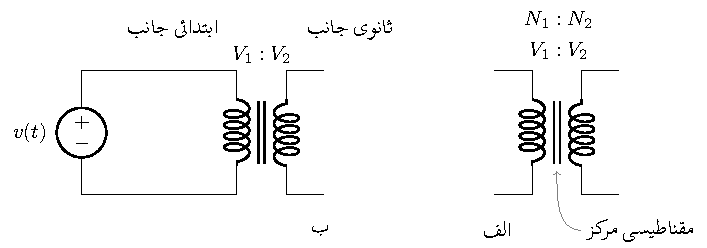
\includegraphics{figTransformersSymbol}
\begin{tikzpicture}
%grid
%\draw[gray,thick] (-4,-4) grid (4,4);
%\draw[help lines,xstep=0.1,ystep=0.1] (-4,-4) grid (4,4);
%symbol only
\begin{scope}[xshift=5cm]
\draw (0,0) node [transformer core](T){}  % reminded by @PaulGessler, thanks.
 %     (T.A1) node[above] {A1}
   %   (T.A2) node[below] {A2}
     % (T.B1) node[above] {B1} 
    %  (T.B2) node[below] {B2}
      (T.base) node[above]{$
\begin{aligned}
N_1& : N_2\\
V_1&:V_2
\end{aligned}
$};
%\draw (T.A1) --++(-2,0);
%\draw (T.A2) --++(-2,0);
%
\draw[<-,gray](0,-1.7) to [out=-90,in=180] (0.4,-2.7) node[right,black] {\RL{مقناطیسی قالب}};
\draw(-1,-2.7) node{الف};
\end{scope}
%transformer powered
\draw (0,0) node [transformer core](T){}  % reminded by @PaulGessler, thanks.
  %    (T.A1) node[above] {A1}
    %  (T.A2) node[below] {A2}
     %(T.B1) node[above] {B1} 
     % (T.B2) node[below] {B2}
      (T.base) node[above]{$V_1:V_2$};
\draw (T.A2) --++(-2,0)   to [american voltage source,l=$v(t)$] ++(0,2.1)--(T.A1);
\draw (-1.5,0.7) node{\RL{ابتدائی جانب}};
\draw(1.5,0.7) node{\RL{ثانوی جانب}};
\draw(1,-2.7) node{ب};
\end{tikzpicture}
\caption{ٹرانسفارمر کی علامت۔}
\label{شکل_ٹرانسفارمر_علامت}
\end{figure}

بڑے ٹرانسفارمر عموماً صرف دو لچھوں پر مشتمل ہوتے ہیں۔اس کتاب میں مقناطیسی قالب پر لپٹے ہوئے دو لچھوں کے  قوی ٹرانسفارمر پر تبصرہ کیا جائے گا۔

ٹرانسفارمر کے کم برقی دباو کے لچھے کو \اصطلاح{کم برقی دباو کا لچھا}\فرہنگ{لچھا!کم برقی دباو}\حاشیہب{low voltage coil}\فرہنگ{coil!low voltage}  کہتے ہیں اور ٹرانسفارمر کی اس جانب کو \اصطلاح{کم برقی دباو والی جانب}  کہتے ہیں جبکہ ٹرانسفارمر کے زیادہ برقی دباو کے لچھے کو \اصطلاح{زیادہ برقی دباو کا لچھا}\فرہنگ{لچھا!زیادہ برقی دباو}\حاشیہب{high voltage coil}\فرہنگ{coil!high voltage}  کہتے ہیں اور ٹرانسفارمر کی اس جانب کو \اصطلاح{زیادہ برقی دباو والی جانب}  کہتے ہیں۔

یوں اگر ٹرانسفارمر کے کم برقی دباو  جانب برقی دباو لاگو کیا جائے اور زیادہ برقی دباو  جانب سے برقی دباو حاصل کیا جائے تو ٹرانسفارمر کی کم برقی دباو  جانب کو ابتدائی جانب کہیں گے اور اس کی زیادہ برقی دباو  جانب کو ثانوی جانب کہیں گے۔

\حصہ{ٹرانسفارمر کی اہمیت}
بدلتے رو کی برقی طاقت  ایک مقام سے دوسرے مقام با آسانی اور نہایت کم برقی طاقت کی ضیاع سے منتقل کی جا سکتی ہے۔یہی اس کی مقبولیت کا راز ہے۔ٹرانسفارمر کے تبادلہ برقی دباو\فرہنگ{برقی دباو!تبادلہ}\حاشیہب{voltage transformation property} کی خصوصیت ایسا کرنے میں کلیدی کردہر ادا کرتی ہے جسے درج ذیل مثال کی مدد سے  سمجھتے ہیں۔
%
\ابتدا{مثال}
شکل \حوالہ{شکل_ٹرانسفارمر_برقی_طاقت_منتقلی}  سے رجوع کریں۔برقی دباو اور برقی رو کی حاصل ضرب برقی طاقت ہوتی ہے:
\begin{figure}
\centering
%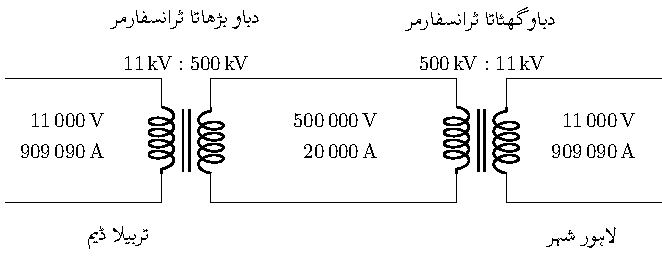
\includegraphics{figTransformersVoltageStepUpBenefits}
\begin{tikzpicture}
%grid
%\draw[gray,thick] (-3,-3) grid (8,2);
%\draw[help lines,xstep=0.1,ystep=0.1] (-3,-3) grid (8,2);
 \pgfmathsetmacro{\height}{0.75}  
%symbol only
\draw (0,0) node [transformer core](Tup){}  % reminded by @PaulGessler, thanks.
 %     (Tup.A1) node[above] {A1}
   %   (Tup.A2) node[below] {A2}
     % (Tup.B1) node[above] {B1} 
    %  (Tup.B2) node[below] {B2}
      (Tup.base) node[above]{$\SI{11}{\kilo \volt}:\SI{500}{\kilo \volt}$};
%\draw (T.A1) --++(-2,0);
%\draw (T.A2) --++(-2,0);
%
\draw (5,0) node [transformer core](Tdn){}  % reminded by @PaulGessler, thanks.
 %     (Tdn.A1) node[above] {A1}
   %   (Tdn.A2) node[below] {A2}
     % (Tdn.B1) node[above] {B1} 
    %  (Tdn.B2) node[below] {B2}
      (Tdn.base) node[above]{$\SI{500}{\kilo \volt}:\SI{11}{\kilo \volt}$};
%
\draw(Tup.B1)--(Tdn.A1);
\draw(Tup.B2)--(Tdn.A2);
\draw(Tup.A1)--++(-2,0);
\draw(Tup.A2)--++(-2,0);
\draw(Tdn.B1)--++(2,0);
\draw(Tdn.B2)--++(2,0);
%text
\draw(-0.5,-2.7)node[left]{\RL{تربیلا ڈیم}};
\draw(6,-2.7)node[right]{\RL{لاہور شہر}};
\draw(0,1)node{\RL{دباو بڑھاتا ٹرانسفارمر}};
\draw(5,1)node{\RL{دباو گھٹاتا ٹرانسفارمر}};
%rating
\draw(-3,-1)node[right]{$
\begin{aligned}
\SI{11000}{\volt}&\\
\SI{45454}{\ampere}&
\end{aligned}
$};
\draw(2.5,-1)node{$
\begin{aligned}
\SI{132000}{\volt}&\\
\SI{3788}{\ampere}&
\end{aligned}
$};
\draw(6,-1)node[right]{$
\begin{aligned}
\SI{11000}{\volt}&\\
\SI{45454}{\ampere}&
\end{aligned}
$};
\end{tikzpicture}%
\caption{برقی طاقت کی منتقلی۔}
\label{شکل_ٹرانسفارمر_برقی_طاقت_منتقلی}
\end{figure}
%
\begin{align*}
p=v_1 i_1 = v_2 i_2
\end{align*}
تصور کریں کہ تربیلا ڈیم  سے \عددی{\SI{500}{\mega\watt}}  برقی طاقت  لاہور\حاشیہد{ضلع صوابی میں بھی لاہور ایک تحصیل ہے لیکن اس شہر کو اتنی طاقت نہیں درکار } شہر کے گھریلو صارفین کو  \عددیء{220} وولٹ پر مہیا کرنی ہے۔اگر ہم اس طاقت کو \عددیء{220}  وولٹ پر ہی منتقل کرنا چاہیں تب برقی رو
\begin{align*}
i=\frac{p}{v}=\frac{\num{500000000}}{220}=\SI{2272727}{\ampere}
\end{align*}
ہو گی۔برقی تار میں کثافتِ برقی رو \عددیء{J_{au}} تقریباً \عددیء{5} ایمپیئر فی مربع ملی میٹر \عددیء{J_{au}=\SI{5}{\ampere \per \milli\meter \squared}}  ممکن ہوتی ہے۔یہ ایک محفوظ کثافتِ برقی رو ہے۔اگر برقی تار میں اس سے زیادہ برقی رو گزاری جائے تو اس کی مزاحمت میں برقی طاقت کے ضیاع سے یہ گرم ہو کر پگھل سکتی ہے۔ اس طرح صفحہ \حوالہصفحہ{مساوات_بنیادی_برقی_رو_کثافت} پر  مساوات \حوالہ{مساوات_بنیادی_برقی_رو_کثافت} سے برقی تار کا رقبہ عمودی تراش
\begin{align*}
A=\frac{i}{J_{au}}=\frac{\num{2272727}}{5}=\SI{454545}{\milli\meter\squared}
\end{align*}
ہو گا۔ گول تار تصور کریں تو اس کا رداس درج ذیل ہو گا۔
\begin{align*}
r=\sqrt{\frac{A}{\pi}}=\sqrt{\frac{\num{454545}}{\pi}}=\SI{380}{\milli\meter}=\SI{0.38}{\meter}
\end{align*}
اتنی موٹی برقی تار کہیں نہیں پائی جاتی ہے\حاشیہد{آپ مانیں یا نہ مانیں، آپ نے بھی اتنی موٹی برقی تار کبھی نہیں دیکھی ہو گی۔}۔اگر یہ تار المونیم کی بنی ہو جس کی  کثافت  \عددیء{\rho_v=\SI{2700}{\kilo\gram\per\meter\cubed}} ہوتی ہے تب ایک میٹر لمبی تار کی کمیت
\begin{align*}
m=2700 \times \pi \times 0.38^2 \times 1=\SI{1224}{\kilo\gram}
\end{align*}
یعنی \عددیء{1.2} ٹن ہو گی۔المونیم اتنی مہنگی ہے کہ اس صورت میں اتنی برقی طاقت کو لاہور پہنچانا ممکن نہیں ہو گا\حاشیہد{آج کل لاہور میں بجلی کی معطلی  اس وجہ سے نہیں ہے۔}۔

آئیں اب ٹرانسفارمر استعمال کر کے دیکھتے ہیں۔ ڈیم پر ایک ٹرانسفارمر نسب کر کے برقی دباو کو بڑھا کر  \عددیء{\num{132000}} وولٹ یعنی \عددیء{132} کلو وولٹ  کیا جاتا ہے۔یوں برقی رو درج ذیل ہو گا
\begin{align*}
i=\frac{p}{v}=\frac{\num{500000000}}{\num{132000}}=\SI{3788}{\ampere}
\end{align*}
جس کے لئے درکار برقی تار
\begin{align*}
A&=\frac{i}{J_{au}}=\frac{\num{3788}}{5}=\SI{758}{\milli\meter\squared}\\
r&=\sqrt{\frac{A}{\pi}}=\sqrt{\frac{1667}{\pi}}=\SI{15.5}{\milli\meter}
\end{align*}
صرف \عددیء{15.5} ملی میٹر رداس کی ہو گی۔ 
\انتہا{مثال}
%

اس مثال میں اگر تربیلا ڈیم میں نسب جنریٹر \عددیء{11000} وولٹ برقی دباو پیدا کر رہا ہو تو تربیلا ڈیم  پر نسب  ٹرانسفارمر برقی دباو کو \عددیء{11000} وولٹ سے بڑھا کر \عددیء{132} کلو وولٹ کرے گا جبکہ لاہور شہر میں نسب  ٹرانسفارمر  \عددیء{132} کلو وولٹ کو واپس \عددیء{11000} وولٹ کرے گا۔

اسی مثال کو بڑھاتے ہیں۔شہر میں \عددیء{220} وولٹ کی بجائے \عددیء{11000} وولٹ صارف کے قریب  پہنچا کر محلہ میں نسب ٹرانسفارمر  کی مدد سے \عددیء{11000}  وولٹ کو مزید گھٹا کر  \عددیء{220} وولٹ کیا جائے گا جو صارف کو فراہم کیے جائیں گے۔  

شکل \حوالہ{شکل_ٹرانسفارمر_برقی_طاقت_منتقلی} میں ڈیم سے شہر تک کا نظام دکھایا گیا ہے جہاں ڈیم پر نسب ٹرانسفارمر کو \اصطلاح{برقی دباو بڑھاتا ٹرانسفارمر}\فرہنگ{ٹرانسفارمر!دباو بڑھاتا}\حاشیہب{step up transformer}\فرہنگ{step up transformer}  اور لاہور میں نسب ٹرانسفارمر کو \اصطلاح{برقی دباو گھٹاتا ٹرانسفارمر}\فرہنگ{ٹرانسفارمر!دباو گھٹاتا}\حاشیہب{step down transformer}\فرہنگ{step down transformer}  کہا گیا ہے۔

برقی طاقت عموماً \عددیء{11} کلو وولٹ اور  \عددیء{25} کلو وولٹ کے مابین پیدا کی جاتی ہے۔اس کی منتقلی  \عددیء{110 } کلو وولٹ اور \عددیء{1000}  کلو وولٹ کے بیچ کی جاتی ہے جبکہ اس کا استعمال  \عددیء{1000} وولٹ سے کم پر کیا جاتا ہے۔

\حصہ{ٹرانسفارمر کے اقسام}
گھروں اور کارخانوں کو برقی طاقت فراہم کرنے والے ٹرانسفارمر مقناطیسی قالب پر لپیٹے جاتے ہیں۔یہ عموماً  \اصطلاح{تین مرحلہ}\فرہنگ{تین مرحلہ}\حاشیہب{three phase}\فرہنگ{three phase} ہوتے ہیں جنہیں  \اصطلاح{لوہے کے قالب والے تین  مرحلہ قوی ٹرانسفارمر}\حاشیہب{iron core, three phase power transformer} کہتے ہیں۔

نہایت چھوٹے ٹرانسفارمر عموماً لوہے کے قالب  پر بنائے جاتے ہیں اور \اصطلاح{یک مرحلہ}\فرہنگ{یک مرحلہ}\حاشیہب{single phase}\فرہنگ{single phase} ہوتے ہیں۔یہ گھریلو استعمال کے برقی مشین، مثلاً موبائل چارجر، وغیرہ میں نسب ہوتے ہیں اور \عددیء{220} وولٹ سے برقی دباو مزید گھٹاتے ہیں۔

برقی دباو کی پیمائش کے لئے مستعمل ٹرانسفارمر، جو \اصطلاح{دباو کے ٹرانسفارمر}\فرہنگ{ٹرانسفارمر!برقی دباو والا}\حاشیہب{potential transformer}  کہلاتے ہیں،   کے  ثانوی  اور ابتدائی  برقی دباو کی تناسب  پر خاص توجہ دی جاتی ہے۔اسی طرح برقی رو کی  پیمائش کے لئے مستعمل ٹرانسفارمر، جو \اصطلاح{رو کے ٹرانسفارمر}\فرہنگ{ٹرانسفارمر!رو والا}\حاشیہب{current transformer}  کہلاتے ہیں،  کے ثانوی اور  ابتدائی  رو کی تناسب پر خاص توجہ دی جاتی ہے۔ ویسے تو ہر ٹرانسفارمر کسی تناسب سے  برقی دباو یا برقی رو کم یا زیادہ کرتا ہے لیکن جیسا پہلے ذکر کیا گیا، ان دو اقسام کے ٹرانسفارمروں میں کم اور زیادہ کرنے کی تناسب پر خاص توجہ دی جاتی ہے۔ان دو اقسام کے ٹرانسفارمروں کی برقی سکت\فرہنگ{برقی سکت}\حاشیہب{electrical rating}\فرہنگ{electrical rating} نہایت کم\حاشیہد{یہ عموماً تقریباً پچیس وولٹ-ایمپیئر سکت رکھتے ہیں۔} ہوتی ہے۔

ٹرانسفارمر کے لچھوں کے مابین مشترکہ مقناطیسی بہاو خلاء کے ذریعہ بھی ممکن ہے۔انہیں \اصطلاح{خلائی قالب ٹرانسفارمر}\فرہنگ{ٹرانسفارمر!خلائی قالب}\حاشیہب{air core transformer}\فرہنگ{transformer!air core}  کہتے ہیں۔ ایسے ٹرانسفارمر ذرائع ابلاغ\فرہنگ{ٹرانسفارمر!ذرائع ابلاغ}\حاشیہب{communication transformer}\فرہنگ{transformer!communication} کے ادوار، یعنی ریڈیو، ٹی وی وغیرہ میں پائے جاتے ہیں۔ان ٹرانسفارمروں کی علامت  شکل \حوالہ{شکل_ٹرانسفارمر_خلائی_قالب_علامت} میں دکھائی گئی ہے  جس میں  قالب ظاہر کرنے والی متوازی لکیریں نہیں پائی جاتی ہیں۔
\begin{figure}
\centering
\begin{minipage}{0.30\textwidth}
\centering
\begin{tikzpicture}
%grid
\draw (0,0) node [transformer ](T){}; 
\end{tikzpicture}
\caption{خلائی ٹرانسفارمر کی علامت۔}
\label{شکل_ٹرانسفارمر_خلائی_قالب_علامت}
\end{minipage}%
\begin{minipage}{0.60\textwidth}
\centering
%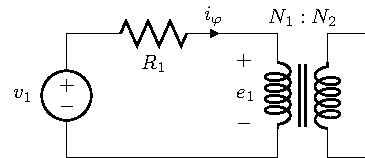
\includegraphics{figTransformersAppliedAndInducedVoltages}
\begin{tikzpicture}
%grid
%\draw[gray,thick] (-4,-4) grid (4,4);
%\draw[help lines,xstep=0.1,ystep=0.1] (-4,-4) grid (4,4);
 \pgfmathsetmacro{\height}{0.75}
%symbol only
\draw (0,0) node [transformer core](T){}  % reminded by @PaulGessler, thanks.
 %     (T.A1) node[above] {A1}
   %   (T.A2) node[below] {A2}
     % (T.B1) node[above] {B1} 
    %  (T.B2) node[below] {B2}
      (T.base) node[above]{$N_1:N_2$};
\draw(T.A2) to [short] (-4cm,-2.1) to [american voltage source,l=$v_1$] (-4,0) to [resistor,l_=$R_1$,i^=$i_\varphi$] (T.A1);
\draw(-1,-1)node{$
\begin{aligned}
&+\\
&e_1\\
&-
\end{aligned}
$};
\end{tikzpicture}
\caption{بیرونی برقی دباو اور اندرونی امالی برقی دباو میں فرق۔}
\label{شکل_ٹرانسفارمر_بیرونی_اور_اندرونی_برقی_دباو}
\end{minipage}
\end{figure}


\حصہ{امالی برقی دباو}\شناخت{حصہ_ٹرانسفارمر_امالی_برقی_دباو}
اس حصے کا بنیادی مقصد بیرونی برقی دباو \عددیء{v}  اور اندرونی امالی برقی دباو  \عددیء{e} میں فرق واضح کرنا اور ان سے متعلق  تکنیکی اصطلاحات کا تعارف  ہے۔

شکل  \حوالہ{شکل_ٹرانسفارمر_بیرونی_اور_اندرونی_برقی_دباو} میں بے بوجھ\فرہنگ{بے بوجھ}\حاشیہب{unloaded} ٹرانسفارمر دکھایا گیا ہے، یعنی اس کا ثانوی لچھا  کھلے دور رکھا گیا ہے۔ ابتدائی لچھے کی مزاحمت \عددی{R_1} ہے جس کو بیرونی جزو دکھایا گیا ہے۔ابتدائی لچھے پر \عددیء{v_1} برقی دباو لاگو کرنے سے ابتدائی لچھے میں ہیجان انگیز\فرہنگ{ہیجان انگیز برقی رو}\حاشیہب{excitation current}\فرہنگ{excitation current} برقی رو \عددیء{i_{\varphi}} گزرے گا۔اس ہیجان انگیز برقی رو سے پیدا مقناطیسی دباو \عددیء{N_1 i_{\varphi}}  قالب میں مقناطیسی بہاو  \عددیء{\varphi} پیدا کے گا۔ یہ بدلتا مقناطیسی بہاو ابتدائی لچھے میں امالی برقی  دباو \عددیء{e_1}  پیدا کرتا ہے جسے درج ذیل مساوات پیش کرتی ہے۔
\begin{align}
e_1=-\frac{\dif \lambda}{\dif t}=-N_1 \frac{\dif \varphi}{\dif t}
\end{align}

 اس مساوات میں
\begin{itemize}
\item
\عددیء{\lambda} ابتدائی لچھے کی مقناطیسی بہاو کے ساتھ ارتباط بہاو ہے،
\item
\عددیء{\varphi} مقناطیسی قالب میں مقناطیسی بہاو جو دونوں لچھوں میں سے گزرتی ہے،
\item
\عددیء{N_1} ابتدائی لچھے کے چکر ہیں۔
\end{itemize}
%

ابتدائی لچھے کی مزاحمت \عددیء{R_1} صفر نہ ہونے کی صورت میں کرخوف کے قانون برائے برقی دباو کے تحت درج ذیل ہو گا۔
\begin{align}\label{مساوات_ٹرانسفارمر_بیرونی_اندرونی_دباو_فرق}
v_1 = i_{\varphi} R_1+e_1
\end{align}
شکل \حوالہ{شکل_ٹرانسفارمر_بیرونی_اور_اندرونی_برقی_دباو} میں اس مزاحمت کو بطور بیرونی جزو، ٹرانسفارمر کے باہر، دکھایا گیا ہے۔اس لچھے کی رستا متعاملہ بھی ہو گی جسے نظرانداز کیا گیا ہے۔عموماً طاقت کے ٹرانسفارمروں اور موٹروں  میں \عددیء{i_{\varphi} R_1} کی قیمت \عددیء{e_1} اور \عددیء{v_1} کی قیمتوں سے بہت کم ہوتی ہے لہٰذا اسے نظرانداز کیا جا سکتا ہے۔ ایسا کرتے ہوئے درج ذیل لکھا جا سکتا ہے۔
\begin{align}\label{مساوات_ٹرانسفارمر_بیرونی_اندرونی_دباو_تقریبا_برابر}
v_1 = e_1=-N_1 \frac{\dif \varphi}{\dif t}
\end{align}

مساوات \حوالہ{مساوات_ٹرانسفارمر_بیرونی_اندرونی_دباو_فرق} سے  ثابت ہوتا ہے کہ بیرونی لاگو برقی دباو \عددیء{v_1} اور اندرونی امالی برقی دباو \عددیء{e_1} دو علیحدہ برقی دباو ہیں۔یہ بات سمجھ لینا بہت ضروری ہے۔مساوات \حوالہ{مساوات_ٹرانسفارمر_بیرونی_اندرونی_دباو_تقریبا_برابر} کے تحت \عددی{v_1} اور \عددی{e_1} کی مطلق قیمتیں  (تقریباً) ایک دوسرے کے برابر ہوتی ہیں\حاشیہد{جس سے طلبہ کی ذہن میں یہ غلط فہمی پیدا ہوتی ہے کہ یہ ایک ہی برقی دباو کے دو مختلف نام ہیں۔}۔مساوات \حوالہ{مساوات_ٹرانسفارمر_بیرونی_اندرونی_دباو_تقریبا_برابر} میں دائیں ہاتھ منفی کی علامت پائی جاتی ہے۔(ہمیں عموماً برقی دباو کی مطلق  قیمت درکار ہوتی ہے نا کہ اس کی علامت لہٰذا اس کتاب میں مساوات \حوالہ{مساوات_ٹرانسفارمر_بیرونی_اندرونی_دباو_تقریبا_برابر}  طرز کی مساواتوں میں دائیں ہاتھ منفی کی علامت عموماً نہیں لکھی گئی ہے۔)

لچھا \اصطلاح{ہیجان}\فرہنگ{ہیجان}\حاشیہب{excite}\فرہنگ{excite} کرنے سے مراد اس پر بیرونی برقی دباو لاگو کرنا ہے  جبکہ لچھے پر لاگو بیرونی برقی دباو کو \اصطلاح{ہیجان انگیز برقی دباو}\فرہنگ{ہیجان انگیز!برقی دباو}\حاشیہب{excitation voltage}\فرہنگ{excitation voltage}  کہتے ہیں۔لچھے  کو \اصطلاح{ہیجان شدہ} لچھا\فرہنگ{ہیجان!لچھا}\حاشیہب{excited coil}\فرہنگ{excited coil} جبکہ اس میں رواں برقی رو کو \اصطلاح{ہیجان انگیز برقی رو}\فرہنگ{ہیجان انگیز!برقی رو}\فرہنگ{excitation current}\حاشیہب{excitation current} کہتے ہیں۔

لچھے میں گزرتی مقناطیسی بہاو کی تبدیلی سے  برقی دباو حاصل کیا جا سکتا ہے۔ ٹرانسفارمروں میں ساکن لچھا سے برقی دباو حاصل کیا جاتا ہے۔ ساکن لچھا سے حاصل برقی دباو کو \اصطلاح{امالی برقی دباو}\فرہنگ{امالی برقی دباو}\حاشیہب{induced voltage}\فرہنگ{induced voltage}  کہتے ہیں۔برقی دباو کا حصول مقناطیسی میدان میں لچھے کی حرکت سے بھی ممکن ہے۔ ایسے برقی دباو کو \اصطلاح{محرک برقی دباو}\فرہنگ{محرک برقی دباو}\حاشیہب{electromotive force, emf}\فرہنگ{electromotive force}  کہتے ہیں۔یاد رہے ان برقی دباو میں کسی قسم کا فرق نہیں ہوتا۔انہیں مختلف نام صرف پہچان کی خاطر دئے جاتے ہیں۔

\حصہ{ہیجان انگیز  برقی رو اور قالبی ضیاع}
جہاں مقناطیسی قالب میں بدلتا مقناطیسی بہاو ثانوی لچھوں میں فائدہ مند برقی دباو پیدا کرتا ہے وہاں یہ مقناطیسی قالب میں نقصان دہ برقی دباو کو بھی جنم دیتا ہے جس سے مقناطیسی قالب میں \اصطلاح{بھنور نما برقی رو}\فرہنگ{بھنور نما!برقی رو}\حاشیہب{eddy currents}\فرہنگ{eddy currents} پیدا ہوتا ہے۔ بھنور نما برقی رو مقناطیسی قالب میں برقی طاقت کے ضیاع کا سبب بنتا ہے جسے \اصطلاح{بھنور نما برقی رو کا ضیاع}\فرہنگ{بھنور نما!ضیاع}\حاشیہب{eddy current loss}\فرہنگ{eddy current loss}  یا  مختصراً \اصطلاح{قالبی ضیاع}\فرہنگ{قالبی ضیاع}\حاشیہب{core loss}\فرہنگ{core loss} کہتے ہیں۔ قالبی ضیاع کو کم سے کم کرنے کے لئے مقناطیسی قالب کو  باریک لوہے کی \اصطلاح{پتریاں}\فرہنگ{پتریاں}\حاشیہب{laminations}\فرہنگ{laminations} تہہ در تہہ رکھ کر بنایا جاتا ہے۔ان پتریوں پر غیر موصل روغن\فرہنگ{روغن}\حاشیہب{enamel}\فرہنگ{enamel} کی تہہ لگائی جاتی ہے تا کہ بھنور نما برقی رو کو روکا جا سکے۔آپ دیکھیں گے کہ برقی مشین کا قالب عموماً اسی طرح بنایا جاتا ہے۔شکل \حوالہ{شکل_مقناطیسی_ادوار_ایم_پانچ_پتری_کا_خط} اور جدول \حوالہ{جدول_مقناطیسی_ادوار_کثافت_بہاو_بالمقابل_شدت}  میں \عددیء{0.3048} ملی میٹر موٹی \تحریر{M5} قالبی پتری کا \عددیء{B-H} مواد دیا گیا ہے۔

شکل \حوالہ{شکل_ٹرانسفارم_تہہ_در_تہہ_مرکز}-الف میں قالبی پتریوں کے دو اشکال دکھائے گئے ہیں۔ان کی صورت کی وجہ سے انہیں \اصطلاح{ایک} اور \اصطلاح{تین}\فرہنگ{ایک، تین پتریاں}\حاشیہب{E,I}\فرہنگ{E,I}  پتری کہتے ہیں۔ شکل \حوالہ{شکل_ٹرانسفارم_تہہ_در_تہہ_مرکز}-ب میں ایک پتریوں اور تین پتریوں   کو دو طرح آپس میں رکھا گیا ہے۔ان دو طریقوں سے انہیں تہہ در تہہ رکھا جاتا ہے۔لہٰذا اگر پہلی تہہ میں ایک دائیں جانب اور تین بائیں جانب رکھا جائے تو اس کے اوپر دوسری تہہ میں ایک کو بائیں جانب اور تین کو دائیں جانب رکھا جائے گا۔تیسری تہہ میں پھر ایک کو دائیں اور تین کو بائیں جانب رکھا جائے گا، وغیرہ۔اسی طرح انہیں جوڑ کر شکل \حوالہ{شکل_ٹرانسفارم_تہہ_در_تہہ_مرکز}-پ میں دکھایا گیا قالب حاصل کیا جاتا ہے۔

\begin{figure}
\centering
%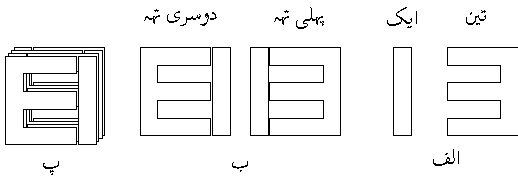
\includegraphics{figTransformersCorePlacement}
\begin{tikzpicture}
%grid
%\draw[gray,thick] (-2,-2) grid (6,2);
%\draw[help lines,xstep=0.1,ystep=0.1] (-2,-2) grid (6,2);
 \pgfmathsetmacro{\t}{0.3}  
\pgfmathsetmacro{\d}{0.9}  
\pgfmathsetmacro{\s}{0.05 cm} 
\begin{scope}[xshift=4cm]
\draw(0,0)--++(0,\t)--++(\d,0)--++(0,\t)--++(-\d,0)--++(0,\t)--++(\d,0)--++(0,\t)--++(-\d,0)--++(0,\t)--++(\d+\t,0)--++(0,-5*\t)--cycle;
\draw(-3*\t,0)--++(0,5*\t)--++(\t,0)--++(0,-5*\t)--cycle;
\draw(-2.5*\t,2)node{ایک};
\draw(0.5,2) node{تین};
\draw(0,-0.1)node[below]{الف};
\end{scope}
%
\begin{scope}[xshift=1cm]
\draw(0,0)--++(0,\t)--++(\d,0)--++(0,\t)--++(-\d,0)--++(0,\t)--++(\d,0)--++(0,\t)--++(-\d,0)--++(0,\t)--++(\d+\t,0)--++(0,-5*\t)--cycle;
\draw(-1.1*\t,0)--++(0,5*\t)--++(\t,0)--++(0,-5*\t)--cycle;
\draw(0.5,2)node{\RL{پہلی تہہ}};
\end{scope}
%
\begin{scope}[x=-1cm,y=1cm]
\draw(0,0)--++(0,\t)--++(\d,0)--++(0,\t)--++(-\d,0)--++(0,\t)--++(\d,0)--++(0,\t)--++(-\d,0)--++(0,\t)--++(\d+\t,0)--++(0,-5*\t)--cycle;
\draw(-1.1*\t,0)--++(0,5*\t)--++(\t,0)--++(0,-5*\t)--cycle;
\draw(0.5,2)node{\RL{دوسری تہہ}};
\draw(-0.5,-0.3)node[below]{ب};
\end{scope}

%stacked core
\begin{scope}[xshift=-3cm,yshift=0cm]
\draw(0.3,-0.3)node[below]{پ};
%bottom layer
\draw[fill=white](0,0)--++(0,\t)--++(\d,0)--++(0,\t)--++(-\d,0)--++(0,\t)--++(\d,0)--++(0,\t)--++(-\d,0)--++(0,\t)--++(\d+\t,0)--++(0,-5*\t)--cycle;
\draw[fill=white](-1.1*\t,0)--++(0,5*\t)--++(\t,0)--++(0,-5*\t)--cycle;
%first layer
\begin{scope}[x=-1cm,y=1cm,xshift=0.88cm-\s,yshift=-\s]
\draw[fill=white](0,0)--++(0,\t)--++(\d,0)--++(0,\t)--++(-\d,0)--++(0,\t)--++(\d,0)--++(0,\t)--++(-\d,0)--++(0,\t)--++(\d+\t,0)--++(0,-5*\t)--cycle;
\draw[fill=white](-1.1*\t,0)--++(0,5*\t)--++(\t,0)--++(0,-5*\t)--cycle;
\end{scope}
%second layer
\begin{scope}[x=1cm,y=1cm,xshift=-2*\s,yshift=-2*\s]
\draw[fill=white](0,0)--++(0,\t)--++(\d,0)--++(0,\t)--++(-\d,0)--++(0,\t)--++(\d,0)--++(0,\t)--++(-\d,0)--++(0,\t)--++(\d+\t,0)--++(0,-5*\t)--cycle;
\draw[fill=white](-1.1*\t,0)--++(0,5*\t)--++(\t,0)--++(0,-5*\t)--cycle;
\end{scope}
%third layer
\begin{scope}[x=-1cm,y=1cm,xshift=0.88cm-3*\s,yshift=-3*\s]
\draw[fill=white](0,0)--++(0,\t)--++(\d,0)--++(0,\t)--++(-\d,0)--++(0,\t)--++(\d,0)--++(0,\t)--++(-\d,0)--++(0,\t)--++(\d+\t,0)--++(0,-5*\t)--cycle;
\draw[fill=white](-1.1*\t,0)--++(0,5*\t)--++(\t,0)--++(0,-5*\t)--cycle;
\end{scope}
\end{scope}
\end{tikzpicture}
\caption{قالبی پتری کے اشکال اور ان کو تہہ در تہہ رکھنے کا طریقہ۔}
\label{شکل_ٹرانسفارم_تہہ_در_تہہ_مرکز}
\end{figure}

ہیجان انگیز برقی رو بے بوجھ اور بوجھ بردار ٹرانسفارمر میں یکساں ہوتا ہے ۔جیسا کہ پہلے بھی ذکر کیا گیا ہے، قوی ٹرانسفارمر اور موٹروں میں برقی دباو اور مقناطیسی بہاو سائن نما ہوتے ہیں جبکہ ان میں ہیجان انگیز برقی رو  غیر سائن نما ہوتا ہے۔ یوں اگر
\begin{gather}
\begin{aligned}
\varphi&=\phi_0 \sin \omega t=\phi_0 \cos \left(\omega t -90\degree \right)\\
\hat{\varphi}&=\phi_0 \phase{-90\degree}
\end{aligned}
\end{gather}
ہو تب
\begin{gather}
\begin{aligned}\label{مساوات_ٹڑانسفارمر_دباو_سمتیہ}
e_1&=N_1 \frac{\dif \varphi}{\dif t}=\omega N_1 \phi_0 \cos \omega t\\
\hat{E_1}&=\omega N_1 \phi_0 \phase{0}
\end{aligned}
\end{gather}
ہو\حاشیہد{اس مساوات میں اور اس کے بعد پوری کتاب میں امالی برقی دباو کے ساتھ منفی  علامت نہیں لگائی گئی ہے۔} گا۔یہاں \عددیء{\phi_0} مقناطیسی بہاو کے حیطہ کو ظاہر کرتی ہے اور \عددیء{\omega} زاویائی تعداد ارتعاش یعنی \عددیء{2 \pi f} کو ظاہر کرتی ہے  جہاں \عددیء{f} تعداد ارتعاش ہے جسے ہرٹز \عددیء{\si{\hertz}} میں ناپا جاتا ہے۔ جیسا شکل \حوالہ{شکل_ٹرانسفارمر_مرکزی_ضیاع_اور_مقناطیسی_رو} میں دکھایا گیا ہے \عددیء{\hat{E_1}} اور \عددیء{\hat{\varphi}} کے بیچ \عددیء{90^{\circ}} کا زاویہ ہو گا۔\عددیء{e_1} برقی دباو  کی موثر قیمت \عددیء{E_{rms}}  
\begin{align}
E_{rms}=\frac{\omega N_1 \phi_0}{\sqrt{2}}=4.44 f N_1 \phi_0
\end{align}
ہے جس سے درج ذیل لکھا جا سکتا ہے۔
\begin{align}\label{مساوات_ٹرانسفارمر_درکار_ہیجان_بہاو}
\phi_0=\frac{E_{rms}}{4.44 f N_1 \phi_0}
\end{align}

یہاں رکھ کر دوبارہ نظرثانی کرتے ہیں۔ اگر ایک  لچھے پر \عددیء{E_{rms}} موثر برقی دباو لاگو کیا جائے تو یہ لچھا اتنا ہیجان انگیز برقی رو \عددیء{i_{\varphi}} گزرنے دیتا ہے جس سے نمودار ہونے والا مقناطیسی بہاو مساوات \حوالہ{مساوات_ٹرانسفارمر_درکار_ہیجان_بہاو}  میں دیے گئے مقناطیسی بہاو \عددیء{\phi_0} کے برابر ہو۔ یہ حقیقت  نہ صرف ٹرانسفارمر بلکہ کسی بھی مقناطیسی دور کے لئے درست اور لازم ہے۔
\begin{figure}
\centering
%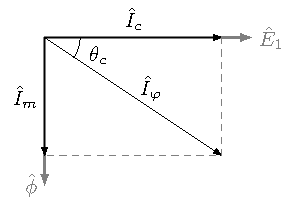
\includegraphics{figTransformersCoreLossAndMagnetizingCurrents}
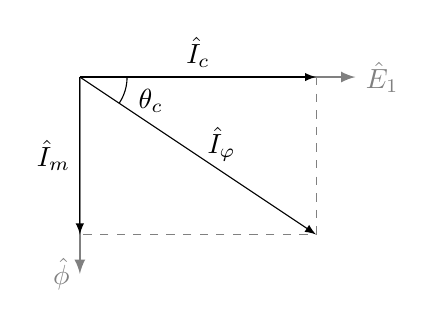
\begin{tikzpicture}
%grid
%\draw[gray,thick] (-2,-2) grid (2,2);
%\draw[help lines,xstep=0.1,ystep=0.1] (-2,-2) grid (2,2);
 \pgfmathsetmacro{\t}{0.3}  
\pgfmathsetmacro{\d}{0.9}  
\pgfmathsetmacro{\s}{0.05 cm} 
\draw[gray,thick,-latex](0,0)--(0,-2.5)node[left]{$\hat{\phi}$};
\draw[gray,thick,-latex](0,0)--(3.5,0)node[right]{$\hat{E}_1$};
\draw[-latex](0,0)--(3,0)node[above,pos=0.5]{$\hat{I}_c$};
\draw[-latex](0,0)--(0,-2)node[left,pos=0.5]{$\hat{I}_m$};
\draw[-latex](0,0)--(3,-2)node[above,pos=0.6]{$\hat{I}_\varphi$};
%
\draw[dashed,gray](3,0)--(3,-2)--(0,-2);
%angle
\begin{scope}
\clip (3,-2)--(0,0)--(3,0);
\draw (0,0) circle (0.6);
\end{scope}
\draw(0.9,-0.3)node {$\theta_c$};
\end{tikzpicture}
\caption{مختلف مرحلی سمتیوں کے زاویے۔}
\label{شکل_ٹرانسفارمر_مرکزی_ضیاع_اور_مقناطیسی_رو}
\end{figure}

غیر سائن نما ہیجان انگیز برقی رو \عددیء{i_{\varphi}} کو \اصطلاح{فوریئر} تسلسل\فرہنگ{فوریئر تسلسل}\حاشیہب{Fourier series}\فرہنگ{Fourier series} سے درج ذیل لکھا جا سکتا ہے۔
\begin{align} 
i_{\varphi}=\sum_n {\left( a_n \cos n \omega t + b_n \sin n\omega t \right)}
\end{align}
اس تسلسل میں \عددیء{(a_1 \cos \omega t+b_1 \sin \omega t)} کو \اصطلاح{بنیادی جزو}\فرہنگ{بنیادی جزو}\حاشیہب{fundamental component}\فرہنگ{fundamental component}  جبکہ باقی حصہ کو  \اصطلاح{موسیقائی جزو}\فرہنگ{موسیقائی جزو}\حاشیہب{harmonic components}\فرہنگ{harmonic components}  کہتے ہیں۔ بنیادی جزو میں \عددیء{a_1 \cos \omega t}، مقناطیسی بہاو سے وجود میں آنے والے امالی برقی دباو، \عددیء{e_1}  (مساوات \حوالہ{مساوات_ٹڑانسفارمر_دباو_سمتیہ})  کے ہم قدم ہے اور  دونوں ایک ساتھ بڑھتے اور گھٹتے ہیں جبکہ  \عددیء{b_1 \sin \omega t} نوے درجہ زاویہ \عددیء{e_1}  کے پیچھے رہتا ہے۔ قالب میں مختلف وجوہات کی بنا برقی طاقت کی ضائع،  کو \عددیء{a_1 \cos \omega t} ظاہر  کرتی ہے۔اسی لئے اس جزو کو \اصطلاح{جزو قالبی ضیاع}\فرہنگ{قالبی ضیاع!جزو}\حاشیہب{core loss component}\فرہنگ{core loss component}  کہتے ہیں۔ہیجان انگیز برقی رو \عددیء{i_{\varphi}} سے \عددیء{a_1 \cos \omega t} منفی کر کے مقناطیس بنانے والا برقی رو یا
 \اصطلاح{مقناطیسی برقی رو}\فرہنگ{مقناطیسی برقی رو}\حاشیہب{magnetizing current}\فرہنگ{magnetizing current}حاصل ہو گا۔ تسلسل  کی تیسری موسیقائی جزو سب سے زیادہ اہم  ہے۔ قوی  ٹرانسفارمروں میں  تیسرا موسیقائی جزو عموماً  کل ہیجان انگیز برقی رو  کا \عددیء{40} فی صد ہوتا ہے۔  

ماسوائے جب  ہیجان انگیز برقی رو کے اثرات پر غور کیا جا رہا ہو، ہم ہیجان انگیز برقی رو کے غیر سائن نما ہونے کو نظرانداز کرتے ہیں۔ قوی ٹرانسفارمر کا  ہیجان انگیز برقی رو اس کے کل برقی رو\حاشیہد{کل برقی رو سے مراد وہ برقی رو ہے جو کل برقی بوجھ لادنے سے حاصل ہوتا ہے۔} کا تقریباً \عددیء{5}  فی صد  ہوتا ہے  لہٰذا  اس کا اثر بہت کم ہوتا ہے۔ یوں ہم  ہیجان انگیز برقی رو کو سائن نما تصور کر کے اس کے اثرات پر غور کرتے ہیں۔ایسا کرنے سے مسئلہ پر غور کرنا آسان ہو جاتا ہے۔ اس فرضی سائن نما  ہیجان انگیز برقی رو\حاشیہد{یعنی  بدلتی برقی رو \عددیء{i_{\varphi}} کو اب مرحلی سمتیہ کی مدد سے \عددیء{\hat{I_{\varphi}}} لکھتے ہیں} \عددیء{\hat{I_{\varphi}}}  کی موثر قیمت \عددیء{I_{\varphi,rms}} ، اصل  ہیجان انگیز برقی رو کی موثر قیمت کے برابر رکھی جاتی ہے جبکہ اس کا زاویہ \عددیء{\theta_c} یوں رکھا جاتا ہے کہ اس سے حاصل برقی ضیاع اصل برقی ضیاع کے برابر ہو۔ شکل \حوالہ{شکل_ٹرانسفارمر_مرکزی_ضیاع_اور_مقناطیسی_رو}  کی مدد سے یہ بات سمجھنی زیادہ آسان ہے۔قالبی ضیاع \عددیء{p_c} ہونے کی صورت میں \عددی{\theta_c} کی قیمت یوں منتخب کی جائے گی کہ درج ذیل مساوات درست ہو۔
\begin{align}
p_c=E_{rms} I_{\varphi,rms} \cos \theta_c
\end{align}
\عددیء{\hat{I_{\varphi}}} دباو  \عددیء{\hat{E_1}} سے \عددی{\theta_c}  پیچھے ہو گا۔

\حصہ{تبادلہ برقی دباو اور تبادلہ برقی رو کے خواص}
ہم شکل \حوالہ{شکل_ٹرانسفارمر_کامل_بار_بردار_ٹرانسفارمر}  کی مدد سے ٹرانسفارمر کا مطالعہ کرتے ہیں۔  ہم فرض کرتے ہیں کہ ابتدائی لچھا  \عددیء{N_1} اور ثانوی لچھا  \عددیء{N_2} چکر کا ہے اور  دونوں لچھوں کی مزاحمتیں صفر ہیں۔ ہم مزید  فرض کرتے  ہیں کہ پورا مقناطیسی بہاو  قالب  میں رہتا  اور دونوں لچھوں سے گزرتا ہے،  قالب میں برقی توانائی ضائع نہیں ہوتی اور قالب کا مقناطیسی مستقل اتنا بڑا ہے کہ ہیجان انگیز برقی رو قابل نظر انداز ہے۔ برقی رو \عددیء{i_1}  اور \عددیء{i_2} کے رخ یوں رکھے گئے ہیں کہ ان سے پیدا مقناطیسی بہاو ایک دوسرے کے مخالف رخ   ہیں۔ اصل ٹرانسفارمر ان باتوں پر تقریباً پورا اترتا ہے۔ ایسے ٹرانسفارمر کو کامل ٹرانسفارمر\فرہنگ{ٹرانسفارمر!کامل}\حاشیہب{ideal transformer}\فرہنگ{transformer!ideal}  کہتے ہیں۔
\begin{figure}
\centering
%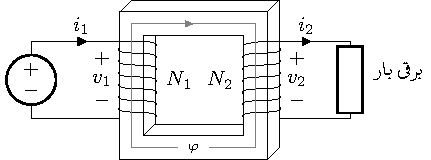
\includegraphics{figTransformersLoadedIdealTransformer}
\begin{tikzpicture}
\def\height{2.5};
\def\width{2.5};
\def\thick{0.4};
\def\depthX{0.2};
\def\depthY{0.2};
\def\gap{0.05};
%grid
%\draw[gray,thick](0,0) grid (5,3);
%\draw[gray,thin,xstep=0.1,ystep=0.1](0,0) grid (5,3);
%going clockwise from origin
\draw(0,0)--++(0,\height)--++(\width,0)--++(0,-\height)--cycle;
\draw(0,0)++(\thick,\thick)--++(0,\height-2*\thick)--++(\width-2*\thick,0)--++(0,-\height+2*\thick)--cycle;
%
\draw(\thick,\thick)--++(\depthX,\depthY) --++(0,\height-2*\thick-\depthY);
\draw(\thick,\thick)--++(\depthX,\depthY) --++(\width-2*\thick-\depthX,0);
\draw(0,\height)--++(\depthX,\depthY)--++(\width,0)--++(-\depthX,-\depthY);
\draw(\width,0)--++(\depthX,\depthY)--++(0,\height)--++(-\depthX,-\depthY);

%left winding
\draw (0.6,1.9) to [out=45,in=0] (0.2,2);% to (-1.5,2);
\foreach \l in {1.9,1.7,1.5,1.3,1.1,0.9}{
\draw (0,\l) to [out=-135,in=45] (0.6,\l-0.2);
}
\draw (0,0.7) to (-1.5,0.7) to [american voltage source] (-1.5,2) to[short,i^=$i_1$] (0.2,2);   %input power
%right  winding
\draw (2.1,1.9) to [out=135,in=0] (2.4,2);% to (-1.5,2);
\foreach \l in {1.9,1.7,1.5,1.3,1.1,0.9}{
\draw (2.7,\l) to [out=-45,in=135] (2.1,\l-0.2);
}
\draw(2.4,2) to [short,i^={$i_2$}] ++(1.5,0) to [european resistor] ++(0,-1.3)--(2.7,0.7);

%flux
\draw[gray,-latex](0.5*\width,\height-0.5*\thick)--++(0.5*\width-0.5*\thick,0)--++(0,-\height+\thick)--++(-\width+\thick,0)--++(0,\height-\thick)
--++(0.5*\width-0.5*\thick,0);
\path[fill=white] (0.35*\width,0.1) rectangle (0.7*\width,0.3); %making roo for writing flux
\draw(0.5*\width,0.5*\thick)node{$\varphi_m$};
%text
\draw (1,1.35)node{$N_1$};
\draw (-0.3,1.35)node{$v_1$};
\draw (-0.3,1.7)node{$+$};
\draw (-0.3,1)node{$-$};
\draw (1.7,1.35)node{$N_2$};
\draw (3,1.35)node{$v_2$};
\draw (3,1.7)node{$+$};
\draw (3,1)node{$-$};
\draw(4.2,1.5)node[right]{\RL{برقی بوجھ}};
\end{tikzpicture}
\caption{کامل بوجھ بردار ٹرانسفارمر۔}
\label{شکل_ٹرانسفارمر_کامل_بار_بردار_ٹرانسفارمر}
\end{figure}

کامل ٹرانسفارمر کے ابتدائی لچھے پر بدلتا برقی دباو \عددیء{v_1} لاگو کرنے سے قالب میں بدلتا مقناطیسی بہاو  \عددیء{\varphi_m} پیدا ہو گا جو ابتدائی لچھے میں ،  لاگو برقی دباو \عددیء{v_1} کے برابر،  امالی برقی دباو \عددیء{e_1} پیدا کرتا ہے۔
\begin{align}\label{مساوات_ٹرانسفارمر_ابتدائی_ثانوی_دباو_الف}
v_1=e_1=N_1 \frac{\dif \varphi_m}{\dif t}
\end{align}
یہی مقناطیسی بہاو دوسرے لچھے سے بھی گزرے گا اور اس میں \عددیء{e_2} امالی برقی دباو پیدا کرے گا جو ثانوی  سروں پر برقی دباو \عددیء{v_2}  کی صورت میں نمودار ہو گا۔
\begin{align}\label{مساوات_ٹرانسفارمر_ابتدائی_ثانوی_دباو_ب}
v_2=e_2=N_2 \frac{\dif \varphi_m}{\dif t}
\end{align}
مساوات \حوالہ{مساوات_ٹرانسفارمر_ابتدائی_ثانوی_دباو_الف} کو مساوات \حوالہ{مساوات_ٹرانسفارمر_ابتدائی_ثانوی_دباو_ب} سے تقسیم کرتے ہوئے درج ذیل رشتہ حاصل ہوتا ہے
\begin{align}\label{مساوات_ٹرانسفارمر_تبادلہ_دباو}
\frac{v_1}{v_2}=\frac{N_1 \frac{\dif \varphi_m}{\dif t}}{N_2 \frac{\dif \varphi_m}{\dif t}}=\frac{N_1}{N_2}
\end{align}
جس کے تحت  کامل ٹرانسفارمر دونوں لچھوں کے چکروں کی نسبت سے \اصطلاح{تبادلہ برقی دباو}\فرہنگ{برقی دباو!تبادلہ}\حاشیہب{voltage transformation}\فرہنگ{voltage!transformation} کرتا ہے۔

کامل ٹرانسفارمر میں طاقت کا ضیاع نہیں ہوتا ہے لہٰذا اس  کو  ابتدائی جانب جتنی برقی طاقت  فراہم کی جائے وہ اتنی  برقی طاقت ثانوی جانب دے گا:
\begin{align}
p=v_1 i_1 = v_2 i_2
\end{align}
درج بالا مساوات سے
\begin{align}
\frac{v_1}{v_2}=\frac{i_2}{i_1}
\end{align}
لکھا جا سکتا ہے جس کو مساوات  \حوالہ{مساوات_ٹرانسفارمر_تبادلہ_دباو} کے ساتھ ملا کر درج ذیل حاصل ہوتا ہے۔
\begin{align}\label{مساوات_ٹرانسفارمر_ابتدائی_ثانوی_دباو_پ}
\frac{v_1}{v_2}=\frac{i_2}{i_1}=\frac{N_1}{N_2}
\end{align}
مساوات \حوالہ{مساوات_ٹرانسفارمر_ابتدائی_ثانوی_دباو_پ}  ٹرانسفارمر کی تبادلہ برقی دباو اور \اصطلاح{تبادلہ برقی رو}\فرہنگ{برقی رو!تبادلہ}\حاشیہب{current transformation}\فرہنگ{current!transformation} کی خاصیت  پیش کرتی ہے جسے عموماً دو حصوں میں یوں لکھا جاتا ہے:
\begin{gather}
\begin{aligned}\label{مساوات_ٹرانسفارمر_تبادلہ_دباو_رو}
\frac{v_1}{v_2}&=\frac{N_1}{N_2}&& \text{\RL{تبادلہ برقی دباو}}\\
\frac{i_1}{i_2}&=\frac{N_2}{N_1}&&\text{\RL{تبادلہ برقی رو}}
\end{aligned}
\end{gather}
اس مساوات کا پہلی جزو کہتا ہے کہ ٹرانسفارمر کی دونوں جانب برقی دباو  دونوں اطراف چکروں کا راست متناسب  ہو گا جبکہ مساوات کا دوسری جزو کہتا ہے کہ ٹرانسفارمر کے دونوں اطراف برقی رو  چکروں کا بالعکس متناسب ہو گا۔

\ابتدا{مثال}
شکل  \حوالہ{شکل_ٹرانسفارمر_کامل_بار_بردار_ٹرانسفارمر}  میں درج ذیل لیتے ہوئے ٹرانسفارمر کی دونوں جانب برقی دباو اور برقی رو معلوم کریں۔
\begin{align*}
\hat{V_1}&=220 \phase{0}\\
N_1:N_2&=220:22\\
Z&=R=\SI{10}{\ohm}
\end{align*}


حل:\quad 
ابتدائی جانب برقی دباو  \عددیء{220} وولٹ دیا گیا ہے۔ ہم  ثانوی جانب برقی دباو کو مساوات \حوالہ{مساوات_ٹرانسفارمر_تبادلہ_دباو_رو} کے پہلی جزو کی مدد سے حاصل کرتے ہیں۔
\begin{align*}
\hat{V_2}=\frac{N_2}{N_1} \hat{V_1}=\frac{22}{220} \times 220\phase {0}=22\phase{0}
\end{align*}
ثانوی دباو \عددیء{22} وولٹ ہے جو ابتدائی  دباو کے ہم قدم ہے۔ثانوی برقی دباو \عددیء{10} اوہم کی مزاحمت میں برقی رو پیدا کرے گا جسے اوہم کے قانون سے حاصل کرتے ہیں:
\begin{align*}
\hat{I_2}=\frac{22 \phase {0}}{10}=2.2\phase {0}
\end{align*}
ثانوی رو \عددیء{2.2} ایمپیئر  ہے۔ ابتدائی رو مساوات \حوالہ{مساوات_ٹرانسفارمر_تبادلہ_دباو_رو} کے دوسری جزو سے حاصل کرتے ہیں۔
\begin{align*}
\hat{I_1}=\frac{N_2}{N_1} \hat{I_2}=\frac{22}{220} \times 2.2\phase{0}=0.22\phase{0}
\end{align*}
\انتہا{مثال}

اس مثال کے نتائج ایک جگہ لکھ کر ان پر غور کرتے ہیں۔
\begin{align*}
\hat{V_1}=220\phase{0}, \quad \hat{V_2}=22\phase{0}, \quad \hat{I_1}=0.22\phase{0}, \quad \hat{I_2}=2.2\phase{0}
\end{align*}
ابتدائی دباو ثانوی  دباو کے دس گنا ہے جبکہ برقی رو میں قصہ الٹ ہے۔ثانوی رو ابتدائی رو کے دس گنا ہے۔طاقت دونوں اطراف  برابر ہے۔یہاں رک کر  اس بات کو اچھی طرح سمجھ لیں کہ جس جانب برقی دباو زیادہ ہوتا ہے اس جانب برقی رو کم ہو گا۔ یوں زیادہ دباو  لچھا کے چکر زیادہ ہوں گے اور اس لچھے میں نسبتاً باریک برقی تار استعمال ہو گی جبکہ کم  دباو لچھا کم چکر کا ہو گا اور اس میں نسبتاً موٹی برقی تار استعمال ہو گی۔ موٹی تار زیادہ رو گزارنے  کی سکت رکھتی ہے۔ 


\ابتدا{مثال}
صفحہ \حوالہصفحہ{شکل_ٹرانسفارمر_رکاوٹ_کا_تبادلہ} پر شکل \حوالہ{شکل_ٹرانسفارمر_رکاوٹ_کا_تبادلہ}-الف  میں رکاوٹ \عددیء{Z_2} کو  بدلتے برقی دباو \عددیء{\hat{V_1}} کے ساتھ ایک ٹرانسفارمر کے ذریعہ جوڑا گیا ہے۔درج ذیل معلومات کی روشنی میں رکاوٹ میں برقی رو اور طاقت کا ضیاع دریافت کریں۔
\begin{align*}
\hat{V_1}=110\phase{0},\quad Z_2=R+j X=3+j 2,\quad N_1:N_2=220:22 
\end{align*}

حل:\quad
ٹرانسفارمر کی تبادلہ برقی دباو کی خاصیت کے تحت ابتدائی  \عددیء{110} وولٹ دباو  ثانوی جانب درج ذیل  دباو \عددیء{\hat{V_s}} دے گا۔
\begin{align*}
\hat{V_s}=\frac{N_2}{N_1} \hat{V_1}=\frac{22}{220} \times 110\phase{0}=11\phase{0}
\end{align*}
یوں ثانوی رو
\begin{align*}
\hat{I_2}=\frac{\hat{V_s}}{Z}=\frac{11\phase{0}}{3+j 2}= 3.05\phase{-33.69\degree}
\end{align*}
اور رکاوٹ میں برقی طاقت کا ضیاع \عددیء{p_z} درج ذیل ہو گا۔
\begin{align*}
p_z=I_2^2 R=3.05^2 \times 3=\SI{27.9}{\watt}
\end{align*}
\انتہا{مثال}

\begin{figure}
\centering
%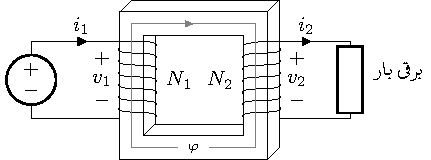
\includegraphics{figTransformersLoadedIdealTransformer}
\begin{tikzpicture}
\def\height{2.5};
\def\width{2.5};
\def\thick{0.4};
\def\depthX{0.2};
\def\depthY{0.2};
\def\gap{0.05};
%grid
%\draw[gray,thick](0,0) grid (5,3);
%\draw[gray,thin,xstep=0.1,ystep=0.1](0,0) grid (5,3);
%going clockwise from origin
\draw(0,0)--++(0,\height)--++(\width,0)--++(0,-\height)--cycle;
\draw(0,0)++(\thick,\thick)--++(0,\height-2*\thick)--++(\width-2*\thick,0)--++(0,-\height+2*\thick)--cycle;
%
\draw(\thick,\thick)--++(\depthX,\depthY) --++(0,\height-2*\thick-\depthY);
\draw(\thick,\thick)--++(\depthX,\depthY) --++(\width-2*\thick-\depthX,0);
\draw(0,\height)--++(\depthX,\depthY)--++(\width,0)--++(-\depthX,-\depthY);
\draw(\width,0)--++(\depthX,\depthY)--++(0,\height)--++(-\depthX,-\depthY);

%left winding
\draw (0.6,1.9) to [out=45,in=0] (0.2,2);% to (-1.5,2);
\foreach \l in {1.9,1.7,1.5,1.3,1.1,0.9}{
\draw (0,\l) to [out=-135,in=45] (0.6,\l-0.2);
}
\draw (0,0.7) to (-2.5,0.7) to [american voltage source,l={$v_1$}] (-2.5,2) to[short,i^=$i_1$]++(0.5,0) to [resistor,l={$R$}]++(2,0) to [short](0.2,2)coordinate(kL); %input
%right  winding
\draw (2.1,1.9) to [out=135,in=0] (2.4,2);% to (-1.5,2);
\foreach \l in {1.9,1.7,1.5,1.3,1.1,0.9}{
\draw (2.7,\l) to [out=-45,in=135] (2.1,\l-0.2);
}
\draw(2.4,2)coordinate(kR) to [short]++(1,0) to [short,i^={$i_2$}] ++(0.5,0) to [european resistor,l={$Z$}] ++(0,-1.3)--(2.7,0.7);
%flux
%\draw[gray,-latex](0.5*\width,\height-0.5*\thick)--++(0.5*\width-0.5*\thick,0)--++(0,-\height+\thick)--++(-\width+\thick,0)--++(0,\height-\thick)--++(0.5*\width-0.5*\thick,0);
%\path[fill=white] (0.4*\width,0.1) rectangle (0.6*\width,0.3); %making roo for writing flux
%\draw(0.5*\width,0.5*\thick)node{$\varphi_m$};
%text
\draw (1,1.35)node{$N_1$};
\draw (-0.3,1.35)node{$e_1$};
\draw (-0.3,1.7)node{$+$};
\draw (-0.3,1)node{$-$};
\draw (1.7,1.35)node{$N_2$};
\draw (3,1.35)node{$e_2$};
\draw (3,1.7)node{$+$};
\draw (3,1)node{$-$};
%\draw(4.2,1.5)node[right]{\RL{برقی بوجھ}};
\end{tikzpicture}
\caption{تبادلہ رو کی خاصیت۔}
\label{شکل_ٹرانسفارمر_تبادلہ_رو_خاصیت}
\end{figure}

\حصہ{ثانوی جانب بوجھ کا ابتدائی جانب اثر}\شناخت{حصہ_ٹرانسفارمر_ثانوی_بار_کا_ابتدائی_جانب_اثر}
شکل \حوالہ{شکل_ٹرانسفارمر_تبادلہ_رو_خاصیت} میں ابتدائی لچھے کی تار کی مزاحمت کو \عددی{R} سے ظاہر کیا گیا ہے جبکہ ثانوی جانب بوجھ \عددی{Z} ہے۔ فرض کریں ہم \عددی{Z}  اتار کر  ٹرانسفارمر کے ثانوی سرے کھلے دور کرتے ہیں۔بے بوجھ ٹرانسفارمر کی ابتدائی جانب بدلتا برقی دباو \عددی{v_1}  لچھے میں ہیجان انگیز برقی رو \عددیء{i_{\varphi}} پیدا کرے گا  جس کا  مقناطیسی دباو \عددیء{N_1 i_{\varphi}} قالب میں گھڑی کے رخ  مقناطیسی بہاو \عددیء{\varphi_m}\حاشیہد{\عددیء{\varphi} کو یہاں \عددیء{\varphi_m} کہا گیا ہے۔} پیدا کرے گا ۔بہاو  \عددیء{\varphi_m} ابتدائی لچھے میں \عددیء{e_1} امالی برقی دباو پیدا کرتا ہے۔
\begin{align}\label{مساوات_ٹرانسفارمر_دباو_برابر_بہاو_تفرق}
e_1=N_1 \frac{\dif \varphi_m}{\dif t}
\end{align}
ابتدائی رو، فراہم کردہ دباو اور ابتدا امالی دباو کا تعلق قانون اہم سے لکھا جا سکتا ہے۔
\begin{align}\label{مساوات_ٹرانسفارمر_امالی_دباو_اور_رو}
i_{\varphi}=\frac{v_1-e_1}{R}
\end{align} 
اب ہم ثانوی جانب  برقی بوجھ \عددی{Z} لادتے ہیں۔  بوجھ بردار ٹرانسفارمر\فرہنگ{ٹرانسفارمر!بوجھ بردار}\حاشیہب{loaded transformer}  کے  ثانوی جانب  برقی رو \عددیء{i_2} رواں ہو گا جس کی وجہ سے \عددیء{N_2 i_2} مقناطیسی دباو وجود میں آئے گا۔ یہ مقناطیسی دباو  قالب میں گھڑی کے مخالف رخ مقناطیسی بہاو \عددیء{\varphi_2}  پیدا کرے گا۔یوں قالب میں  مقناطیسی بہاو تبدیل  ہو کر  (گھٹ کر)
 \عددیء{\varphi_{\text{نیا}}=\varphi_{m}-\varphi_2} اور ابتدائی لچھے میں امالی دباو گھٹ کر \عددیء{e_{\textup{نیا}}} ہو جائے گا۔ مساوات \حوالہ{مساوات_ٹرانسفارمر_امالی_دباو_اور_رو} کے تحت امالی دباو گھٹنے کی وجہ سے ابتدائی رو  بڑھے گا۔ 

آپ نے دیکھا کہ ثانوی جانب کا رو قالب میں مقناطیسی بہاو  تبدیل کر کے ابتدائی لچھے کو بوجھ کے بارے میں خبردار کرتا ہے۔

آئیں \عددی{R} کی قیمت کو نظرانداز کرتے ہوئے بے بار ٹرانسفارمر سے شروع کر کے اس عمل کو زیادہ باریکی سے دیکھیں۔ٹرانسفارمر کو \عددی{v_1} فراہم کرنے سے ابتدائی لچھے میں ہیجان انگیز رو \عددی{i_{\varphi}} پیدا ہو گا جو قالب پر \عددی{N_1i_{\varphi}} مقناطیسی دباو مسلط  کر کے اس میں گھڑی کے رخ بہاو \عددی{\varphi_m} پیدا کرے گا۔ یہ بہاو  لچھے میں امالی دباو \عددی{e_1} پیدا کرتا ہے۔ابتدائی لچھے کی مزاحمت نظرانداز کرتے ہوئے \عددی{v_1=e_1} ہو گا  لہٰذا  مساوات \حوالہ{مساوات_ٹرانسفارمر_دباو_برابر_بہاو_تفرق} درج ذیل صورت اختیار کرتی ہے۔
\begin{align}\label{مساوات_ٹرانسفارمر_دباو_برابر_بہاو_تفرق_ب}
v_1=e_1=N_1 \frac{\dif \varphi_m}{\dif t}
\end{align}
اب ٹرانسفارمر پر \عددی{Z} بوجھ ڈالتے ہیں۔ اس بوجھ کی بنا ثانوی لچھے میں \عددی{i_2} رو پیدا ہو گا جو قالب پر گھڑی کے مخالف رخ مقناطیسی دباو \عددی{N_2i_2} مسلط کر کے اس میں گھڑی کے مخالف رخ بہاو \عددی{\varphi_{2}} پیدا کرے گا۔ اگر \عددی{\varphi_{2}} کا کچھ نہ کیا جائے تب  قالب میں کل مقناطیسی بہاو گھٹ کر \عددی{\varphi_m-\varphi_{2}} ہو جائے گا اور ابتدائی لچھے میں امالی دباو گھٹ جائے گا۔ مساوات \حوالہ{مساوات_ٹرانسفارمر_دباو_برابر_بہاو_تفرق_ب} کے تحت یہ ایک ناممکن صورت حال ہے چونکہ \عددی{e_1} کو ہر صورت \عددی{v_1} کے برابر ہونا ہو گا (یاد رہے \عددی{v_1} کی قیمت جوں کی توں ہے)۔ لہٰذا \عددیء{\varphi_{2}}  کے اثر کو ختم کرنے کے لئے ابتدائی لچھے میں برقی رو \عددیء{i_{1}} نمودار ہو گا جس سے پیدا مقناطیسی دباو \عددی{N_1i_1} مقناطیسی دباو  \عددیء{N_2 i_2} کے اثر کو ختم کر دے گا۔یوں \عددی{N_1i_1} اور \عددی{N_2i_2} کا مجموعی مقناطیسی دباو صفر ہو گا۔
\begin{align}\label{مساوات_ٹرانسفارمر_رو_تناسب}
N_1 i_1-N_2 i_2=0
\end{align}
درج بالا مساوات میں دونوں دباو  ایک دوسرے کے مخالف  رخ ہیں لہٰذا ان کا مجموعہ درحقیقت ان کے فرق کے برابر ہو گا۔مقناطیسی دباو \عددی{N_1i_1} اور \عددی{N_2i_2} قالب میں ایک دوسرے کے مخالف رخ ہیں لہٰذا یہ ایک دوسرے کے اثر کو مکمل طور پر ختم کرتے ہیں۔ یوں بے بوجھ اور بوجھ بردار ٹرانسفارمر دونوں میں  مقناطیسی بہاو \عددیء{\varphi_m}  کے برابر  ہو گا۔ مساوات \حوالہ{مساوات_ٹرانسفارمر_رو_تناسب} سے تبادلہ رو کا کلیہ اخذ کیا جا سکتا ہے:
\begin{align}\label{مساوات_ٹرانسفارمر_برقی_رو_اور_چکر_شرح}
\frac{i_1}{i_2}=\frac{N_2}{N_1}
\end{align}
%

\حصہ{ٹرانسفارمر کی علامت پر نقطوں کا مطلب}
شکل \حوالہ{شکل_ٹرانسفارمر_نقطوں_کی_اہمیت}  میں جس لمحہ پر ابتدائی لچھے کا بالائی سر مثبت برقی دباو پر ہو، اس لمحہ پر ثانوی لچھے کا بالائی سر مثبت دباو پر ہے۔ اس حقیقت کو لچھوں پر نقطوں سے ظاہر کیا گیا ہے۔ یوں نقطی سروں پر دباو ہم قدم ہوں گے۔

 مزید ابتدائی لچھے  کے نقطی سر سے  مثبت برقی رو لچھے میں داخل جبکہ ثانوی لچھے  کے نقطی سر سے  مثبت برقی رو لچھے سے  خارج ہو گی۔

\begin{figure}
\centering
%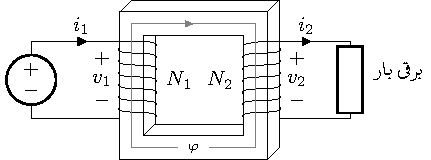
\includegraphics{figTransformersLoadedIdealTransformer}
\begin{tikzpicture}
\def\height{2.5};
\def\width{2.5};
\def\thick{0.4};
\def\depthX{0.2};
\def\depthY{0.2};
\def\gap{0.05};
%grid
%\draw[gray,thick](0,0) grid (5,3);
%\draw[gray,thin,xstep=0.1,ystep=0.1](0,0) grid (5,3);
%going clockwise from origin
\draw(0,0)--++(0,\height)--++(\width,0)--++(0,-\height)--cycle;
\draw(0,0)++(\thick,\thick)--++(0,\height-2*\thick)--++(\width-2*\thick,0)--++(0,-\height+2*\thick)--cycle;
%
\draw(\thick,\thick)--++(\depthX,\depthY) --++(0,\height-2*\thick-\depthY);
\draw(\thick,\thick)--++(\depthX,\depthY) --++(\width-2*\thick-\depthX,0);
\draw(0,\height)--++(\depthX,\depthY)--++(\width,0)--++(-\depthX,-\depthY);
\draw(\width,0)--++(\depthX,\depthY)--++(0,\height)--++(-\depthX,-\depthY);

%left winding
\draw (0.6,1.9) to [out=45,in=0] (0.2,2);% to (-1.5,2);
\foreach \l in {1.9,1.7,1.5,1.3,1.1,0.9}{
\draw (0,\l) to [out=-135,in=45] (0.6,\l-0.2);
}
\draw (0,0.7) to (-1.5,0.7) to [american voltage source] (-1.5,2) to[short,i^=$i_1$]++(0.5,0)to [short] (0.2,2)coordinate(kL); %input
\draw(kL)++(-0.5,0.2)node[circ]{};
%right  winding
\draw (2.1,1.9) to [out=135,in=0] (2.4,2);% to (-1.5,2);
\foreach \l in {1.9,1.7,1.5,1.3,1.1,0.9}{
\draw (2.7,\l) to [out=-45,in=135] (2.1,\l-0.2);
}
\draw(2.4,2)coordinate(kR) to [short]++(1,0) to [short,i^={$i_2$}] ++(0.5,0) to [european resistor] ++(0,-1.3)--(2.7,0.7);
\draw(kR)++(0.5,0.2)node[circ]{};
%flux
%\draw[gray,-latex](0.5*\width,\height-0.5*\thick)--++(0.5*\width-0.5*\thick,0)--++(0,-\height+\thick)--++(-\width+\thick,0)--++(0,\height-\thick)--++(0.5*\width-0.5*\thick,0);
%\path[fill=white] (0.4*\width,0.1) rectangle (0.6*\width,0.3); %making roo for writing flux
%\draw(0.5*\width,0.5*\thick)node{$\varphi_m$};
%text
%\draw (1,1.35)node{$N_1$};
\draw (-0.3,1.35)node{$v_1$};
\draw (-0.3,1.7)node{$+$};
\draw (-0.3,1)node{$-$};
%\draw (1.7,1.35)node{$N_2$};
\draw (3,1.35)node{$v_2$};
\draw (3,1.7)node{$+$};
\draw (3,1)node{$-$};
\draw(4.2,1.5)node[right]{\RL{برقی بوجھ}};
\end{tikzpicture}
\caption{ٹرانسفارمر کی علامت میں نقطوں کا مفہوم۔}
\label{شکل_ٹرانسفارمر_نقطوں_کی_اہمیت}
\end{figure}

\حصہ{رکاوٹ کا تبادلہ}
اس حصہ میں کامل ٹرانسفارمر میں رکاوٹ کے تبادلہ پر غور کیا جائے گا۔شکل \حوالہ{شکل_ٹرانسفارمر_رکاوٹ_کا_تبادلہ}-الف میں ایک ٹرانسفارمر دکھایا گیا ہے جس کی ابتدائی جانب سائن نما برقی دباو  \عددیء{\hat{V_1}=V_1\phase{\theta}}  لاگو کیا گیا ہے۔یہاں مرحلی سمتیہ استعمال کئے جائیں گے۔ٹرانسفارمر پر نقطے ہم قدم سروں کی نشاندہی کرتے ہیں۔

جیسے اوپر ذکر ہوا، برقی دباو \عددیء{\hat{V_1}} اور \عددیء{\hat{V_2}} آپس میں ہم قدم ہیں اور  اسی طرح برقی رو \عددیء{\hat{I_1}} اور \عددیء{\hat{I_2}} آپس میں  ہم قدم ہیں۔مساوات \حوالہ{مساوات_ٹرانسفارمر_تبادلہ_دباو} اور  مساوات \حوالہ{مساوات_ٹرانسفارمر_برقی_رو_اور_چکر_شرح}   کو مرحلی سمتیہ کی مدد سے لکھتے ہیں۔
\begin{gather}
\begin{aligned}\label{مساوات_ٹرانسفارمر_دباو_رو_الف}
\hat{V_1}&=\left(\frac{N_1}{N_2} \right) \hat{V_2}\\
\hat{I_1}&=\left(\frac{N_2}{N_1} \right) \hat{I_2}
\end{aligned}
\end{gather}
خارجی دباو، رو اور رکاوٹ کا تعلق قانون اہم سے لکھتے ہیں۔
\begin{align}
Z_2=\frac{\hat{V_2}}{\hat{I_2}}=\abs{Z_2}\phase{\theta_z}
\end{align}
مساوات \حوالہ{مساوات_ٹرانسفارمر_دباو_رو_الف}  سے درج ذیل لکھا جا سکتا ہے جہاں آخری قدم پر رکاوٹ کی قیمت پر کی گئی ہے۔
\begin{align}\label{مساوات_ٹرانسفارمر_تبادلہ_رکاوٹ_الف}
\frac{\hat{V_1}}{\hat{I_1}}=\left(\frac{N_1}{N_2} \right)^2 \frac{\hat{V_2}}{\hat{I_2}}=\left(\frac{N_1}{N_2} \right)^2  Z_2
\end{align}
یوں  داخلی رو درج ذیل ہو گا۔
\begin{align}\label{مساوات_ٹرانسفارمر_تبادلہ_رکاوٹ_ب}
\hat{I_1}=\frac{\hat{V_1}}{(N_1/N_2 )^2  Z_2}
\end{align}

شکل \حوالہ{شکل_ٹرانسفارمر_رکاوٹ_کا_تبادلہ}-ب میں \عددیء{\hat{V_1}} درج ذیل قیمت کے رکاوٹ \عددیء{Z_2'} کو فراہم کیا گیا ہے۔ 
\begin{align}\label{مساوات_ٹرانسفارمر_متبادل_رکاوٹ_تعریف}
Z_2'=\left(\frac{N_1}{N_2} \right)^2  Z_2
\end{align}
آپ تسلی کر لیں کہ اس دور میں بھی  \عددی{\hat{V_1}} کا برقی رو مساوات \حوالہ{مساوات_ٹرانسفارمر_تبادلہ_رکاوٹ_ب} دیتی ہے۔

مساوات \حوالہ{مساوات_ٹرانسفارمر_تبادلہ_رکاوٹ_ب} سے نسبت \عددی{\tfrac{\hat{V_1}}{\hat{I_1}}} لکھتے ہیں جو شکل \حوالہ{شکل_ٹرانسفارمر_رکاوٹ_کا_تبادلہ}-ب کے تحت \عددی{Z_2'} کے برابر ہے۔ 
\begin{align}\label{مساوات_ٹرانسفارمر_تبادلہ_رکاوٹ_پ}
\frac{\hat{V_1}}{\hat{I_1}}=Z_2'=\left(\frac{N_1}{N_2} \right)^2  Z_2
\end{align}
دونوں ادوار سے  \عددیء{\hat{V_1}} کی طاقت درج ذیل حاصل ہوتی ہے۔
\begin{align}
p=\hat{V_1} \cdot \hat{I_1}=\frac{V_1^2 \cos \theta_z}{\left(\frac{N_1}{N_2} \right)^2  \abs{Z_2}}
\end{align}
%
\begin{figure}
\centering
%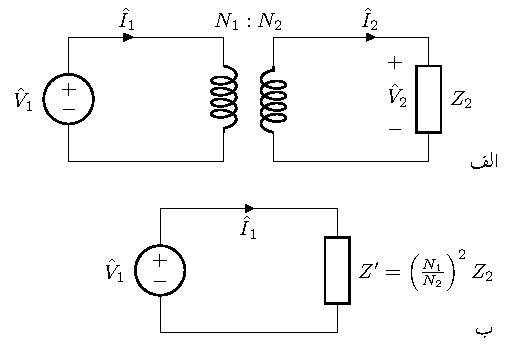
\includegraphics{figTransformersImpedanceTransformation}
\begin{tikzpicture}
%grid
%\draw[gray,thick] (-3,-3) grid (3,3);
%\draw[gray,thin,xstep=0.1,ystep=0.1] (-3,-3) grid (3,3);
%transformer outer dimensions
\pgfmathsetmacro{\h}{2.5}
\begin{scope}[xshift=1.5cm,yshift=5cm]
\draw (0,0) node [transformer] (T1){};
\draw (T1.base)node[above] {$N_1:N_2$};
\draw(T1.A2) to [short] ++(-2,0) to [american voltage source,l=$\hat{V}_1$] ++(0,2.1) to  [short,i^=$\hat{I}_1$]  (T1.A1);
\draw(T1.B1) to [short,i^=$\hat{I}_2$] ++(2,0) to [european resistor,l=$Z_2$] ++(0,-2.1) to (T1.B2);
\draw(T1.A1)++(0.25,-0.2)node[circ]{};
\draw(T1.B1)++(-0.25,-0.2)node[circ]{};
%text
\draw(2.5,-1) node{$
\begin{aligned}
&+\\
&\hat{V}_2\\
&-
\end{aligned}
$};
%urdu
\draw (4,-2.1) node {الف};
\end{scope}
%
\draw (0,0) to [american voltage source,l=$\hat{V}_1$] ++(0,2.1) to [short,i_=$\hat{I}_1$] ++(3,0) to [european resistor,l=${Z_2'=\big(\frac{N_1}{N_2} \big)^2 Z_2}$] ++(0,-2.1) to (0,0);
%urdu
\draw (5.5,0) node {ب};
\end{tikzpicture}
\caption{ٹرانسفارمر کی خاصیت تبادلہ رکاوٹ۔}
\label{شکل_ٹرانسفارمر_رکاوٹ_کا_تبادلہ}
\end{figure}

یوں حساب کرنے کے نقطہ نظر سے  ہم \عددی{\hat{V_1}} کو  مساوات \حوالہ{مساوات_ٹرانسفارمر_متبادل_رکاوٹ_تعریف} میں دی گئی قیمت کے رکاوٹ \عددی{Z_2'} پر لاگو کرتے ہوئے \عددی{\hat{V_1}} کا برقی رو اور  طاقت جان سکتے ہیں۔

منبع \عددی{\hat{V_1}} کو شکل \حوالہ{شکل_ٹرانسفارمر_رکاوٹ_کا_تبادلہ}-الف اور ب میں کوئی فرق نظر نہیں آتا ہے۔اس کے ساتھ ٹرانسفارمر کے ذریعہ \عددی{Z_2} جوڑنا یا بغیر ٹرانسفارمر \عددی{Z_2'} جوڑنا ایک برابر ہے۔  ٹرانسفارمر \عددی{Z_2} کو یوں تبدیل کرتا ہے کہ \عددی{\hat{V_1}} کو رکاوٹ \عددی{Z_2'} نظر آتا ہے۔ ٹرانسفارمر کی اس خاصیت کو  \اصطلاح{تبادلہ رکاوٹ}\فرہنگ{تبادلہ!رکاوٹ}\حاشیہب{impedance transformation}\فرہنگ{impedance transformation} کی خاصیت  کہتے ہیں جس کو درج ذیل مساوات بیان کرتی ہے۔
\begin{align}
Z_2'=\left(\frac{N_1}{N_2} \right)^2  Z_2
\end{align}
ہم حساب کرنے کی خاطر رکاوٹ کو  ٹرانسفارمر کی ایک جانب سے  دوسری جانب منتقل کر سکتے ہیں۔ 
%
\ابتدا{مثال}
شکل \حوالہ{شکل_ٹرانسفارمر_برقی_طاقت_کی_منتقلی}-الف میں رکاوٹ \عددیء{Z_B} کا برقی بوجھ ایک جنریٹر پر لدا ہے۔بوجھ تک برقی طاقت دو برقی تاروں کے ذریعہ منتقل کیا گیا ہے۔ان تاروں کا مجموعہ رکاوٹ \عددیء{Z_t} ہے۔
\begin{figure}
\centering
%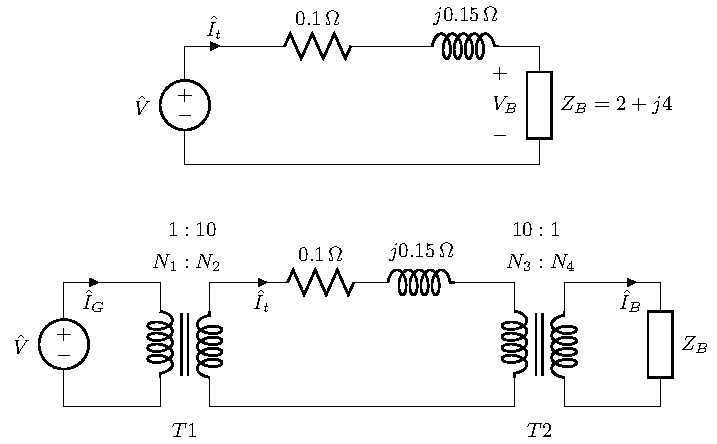
\includegraphics{figTransformersPowerTransmission}
\begin{tikzpicture}
%grid
%\draw[gray,thick](-3,-3) grid (7,3);
%\draw[gray,thin,xstep=0.1,ystep=0.1](-3,-3) grid (7,3);
%
\begin{scope}[yshift=2cm]
%going clockwise from origin
\draw(0,0) to [american voltage source,l=$\hat{V}$] (0,2) to [short,i^=$\hat{I}_t$] ++(1,0) to [resistor,l=$\SI{0.1}{\ohm}$] ++(2.5,0) to [inductor,l=$j\SI{0.15}{\ohm}$] ++(2.5,0) to [european resistor,l=${Z_B=2+j4}$] ++(0,-2) to [short] (0,0);
%text
\draw(5.4,1) node{$
\begin{aligned}
&+\\
&V_B\\
&-
\end{aligned}
$};
\end{scope}
%
\draw (0,0) node [transformer core](T1){}  % reminded by @PaulGessler, thanks.
 %     (T1.A1) node[above] {A1}
   %   (T1.A2) node[below] {A2}
     % (T1.B1) node[above] {B1} 
    %  (T1.B2) node[below] {B2}
      (T1.base) node[above]{$
\begin{aligned}
1&:10\\
N_1&:N_2
\end{aligned}
$};
\draw (6,0) node [transformer core](T2){}  % reminded by @PaulGessler, thanks.
 %     (T2.A1) node[above] {A1}
   %   (T2.A2) node[below] {A2}
     % (T2.B1) node[above] {B1} 
    %  (T2.B2) node[below] {B2}
      (T2.base) node[above]{$
\begin{aligned}
10&:1\\
N_3&:N_4
\end{aligned}
$};
%going clockwise from origin
\draw (T1.B1) to [short,i_=$\hat{I}_t$] ++(0.5,0) to [resistor,l=$\SI{0.1}{\ohm}$] ++(1.5,0) to [inductor,l=$j\SI{0.15}{\ohm}$] (T2.A1) ;
\draw(T1.B2) to (T2.A2);
%
\draw(T1.A2)--++(-1,0) to [american voltage source,l=$\hat{V}$] ++(0,2.1) [short,i_=$\hat{I}_G$] to (T1.A1);
%
\draw(T2.B1) to [short,i_=$\hat{I}_B$] ++(1,0) to [european resistor,l=$Z_B$] ++(0,-2.1) to (T2.B2);
\draw(0,-2.5) node{$T1$};
\draw(6,-2.5) node{$T2$};
\end{tikzpicture}
\caption{برقی طاقت کی منتقلی۔}
\label{شکل_ٹرانسفارمر_برقی_طاقت_کی_منتقلی}
\end{figure}
%
\begin{figure}
\centering
%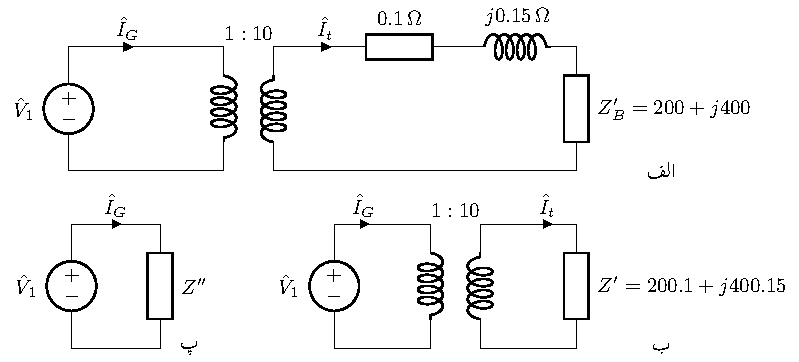
\includegraphics{figTransformersStepByStepSolution}
\begin{tikzpicture}
%grid
%\draw[gray,thick] (-3,-3) grid (7,3);
%\draw[gray,thin,xstep=0.1,ystep=0.1] (-3,-3) grid (7,3);
%transformer outer dimensions
\pgfmathsetmacro{\h}{2.5}
\begin{scope}[xshift=0cm,yshift=3cm]
\draw (0,0) node [transformer] (T1){};
\draw (T1.base)node[above] {$1:10$};
\draw(T1.A2) to [short] ++(-2,0) to [american voltage source,l=$\hat{V}_1$] ++(0,2.1) to  [short,i^=$\hat{I}_G$]  (T1.A1);
\draw(T1.B1) to  [short,i>=$\hat{I}_t$] ++(0.5,0) to [european resistor,l=$\SI{0.1}{\ohm}$] ++(2,0) to [inductor,l=$j\SI{0.15}{\ohm}$] ++(2,0) to [european resistor,l=${Z_B'=200+j 400}$] ++(0,-2.1) to (T1.B2);
%urdu
\draw (7,-2.1) node {الف};
\end{scope}
%
\begin{scope}[xshift=3.5cm,yshift=0cm]
\draw (0,0) node [transformer] (T1){};
\draw (T1.base)node[above] {$1:10$};
\draw(T1.A2) to [short] ++(-1,0) to [american voltage source,l=$\hat{V}_1$] ++(0,2.1) to  [short,i^=$\hat{I}_G$]  (T1.A1);
\draw(T1.B1) to  [short,i>=$\hat{I}_t$]++(1,0) to [european resistor,l=${Z'=200.1+j400.15}$] ++(0,-2.1) to (T1.B2);
%urdu
\draw (3.5,-2.1) node {ب};
\end{scope}
%
\begin{scope}[xshift=-3cm,yshift=-2.1cm]
\draw(0,0)  to [american voltage source,l=$\hat{V}_1$] ++(0,2.1) to  [short,i^=$\hat{I}_G$]  ++(1.5,0) to [european resistor,l=$Z''$] ++(0,-2.1) to [short] (0,0);
%urdu
\draw (2,0) node {پ};
\end{scope}
\end{tikzpicture}
\caption{ٹرانسفارمر قدم با قدم حل کرنے کا طریقہ۔}
\label{شکل_ٹرانسفارمر_قدم_با_قدم_حل}
\end{figure}

شکل-ب میں جنریٹر کے قریب نسب برقی دباو بڑھانے والا ٹرانسفارمر برقی دباو کو دس گنا بڑھاتا ہے اور برقی بوجھ کے قریب نسب برقی دباو گھٹانے والا ٹرانسفارمر برقی دباو کو دس گنا گھٹاتا ہے۔دونوں ٹرانسفارمروں کے بیچ تاروں کا مجموعہ رکاوٹ \عددیء{Z_t}  ہے جبکہ باقی مستعمل تاروں کی رکاوٹ قابل نظر انداز  ہے۔دونوں اشکال میں
\begin{align*}
Z_B=2+j 4, \quad Z_t=0.1 +j 0.15, \quad \hat{V}=415\phase{0}
\end{align*}
لیتے ہوئے 
\begin{itemize}
\item
برقی بوجھ پر برقی دباو معلوم کریں،
\item
برقی تاروں میں برقی طاقت کا ضیاع معلوم کریں۔
\end{itemize}

حل الف:
\begin{align*}
\hat{I_t}&=\frac{\hat{V}}{Z_t+Z_B}=\frac{415\phase{0}}{0.1+j 0.15+2+j 4}\\
&=\frac{415\phase{0}}{2.1+j 4.15}=89.23\phase{-63.159\degree}\\
&=40.3-j79.6
\end{align*}
یوں رکاوٹ پر برقی دباو
\begin{align*}
\hat{V_B}=\hat{I_B} Z_B&=\left(40.3-j79.6 \right) \left( 2+j 4\right)\\
&=399+j2=399\phase{0.287\degree}
\end{align*}
اور برقی تاروں میں برقی طاقت کا ضیاع درج ذیل ہو گا۔
\begin{align*}
p_t=I_t^2 R_t=89.23^2 \times 0.1=\SI{796}{\watt}
\end{align*}

حل ب:\quad
شکل \حوالہ{شکل_ٹرانسفارمر_برقی_طاقت_کی_منتقلی} اور شکل \حوالہ{شکل_ٹرانسفارمر_قدم_با_قدم_حل}  سے رجوع کریں۔شکل  \حوالہ{شکل_ٹرانسفارمر_برقی_طاقت_کی_منتقلی} میں ٹرانسفارمر \عددیء{T_2} کے ثانوی  رکاوٹ کو مساوات \حوالہ{مساوات_ٹرانسفارمر_متبادل_رکاوٹ_تعریف}  کی مدد سے  ابتدائی جانب منتقل کرتے ہیں۔
\begin{align*}
Z_B'=\left(\frac{N_3}{N_4} \right)^2 Z_B=\left(\frac{10}{1} \right)^2 \left(2+j 4 \right)=200+j 400
\end{align*}
یوں شکل \حوالہ{شکل_ٹرانسفارمر_قدم_با_قدم_حل}-الف حاصل ہوتا ہے جس  میں  برقی تار کا رکاوٹ اور  تبادلہ شدہ رکاوٹ سلسلہ وار جڑے ہیں۔ان کے مجموعہ  کو \عددیء{Z'} 
\begin{align*}
Z'=Z_t+Z_B'=0.1+j 0.15+200+j 400=200.1+j400.15
\end{align*}
لکھتے ہوئے شکل \حوالہ{شکل_ٹرانسفارمر_قدم_با_قدم_حل}-ب حاصل ہوتا ہے۔ایک مرتبہ دوبارہ مساوات \حوالہ{مساوات_ٹرانسفارمر_متبادل_رکاوٹ_تعریف}  استعمال کرتے ہوئے \عددی{Z'} کو ٹرانسفارمر کے ابتدائی جانب منتقل کرتے ہوئے
\begin{align*}
Z''=\left(\frac{N_1}{N_2} \right)^2 Z'=\left(\frac{1}{10} \right)^2 \left(200.1+j400.15 \right)=2.001+j4.0015
\end{align*}
شکل \حوالہ{شکل_ٹرانسفارمر_قدم_با_قدم_حل}-پ حاصل ہو گا جس سے جنریٹر کا برقی رو درج ذیل ہو گا۔
\begin{align*}
\hat{I_G}=\frac{\hat{V}}{Z''}=\frac{415\phase{0}}{2.001+j4.0015}=92.76\phase{-63.432\degree}
\end{align*}
شکل \حوالہ{شکل_ٹرانسفارمر_قدم_با_قدم_حل}-ب  میں جنریٹر کا برقی رو جانتے ہوئے  تبادلہ برقی رو سے \عددی{\hat{I_t}} حاصل کرتے ہیں۔
\begin{align*}
\hat{I_t}=\left(\frac{N_1}{N_2} \right) \hat{I_G}=\left(\frac{1}{10}\right) 92.76\phase{-63.432\degree}=9.276\phase{-63.432\degree}
\end{align*}
یوں برقی تار میں طاقت کا ضیاع درج ذیل ہو گا۔
\begin{align*}
p_t=I_t^2 R_t=9.276^2  \times 0.1=\SI{8.6}{\watt}
\end{align*}
اسی طرح شکل \حوالہ{شکل_ٹرانسفارمر_برقی_طاقت_کی_منتقلی}  میں  \عددیء{\hat{I_t}} جانتے ہوئے تبادلہ برقی رو سے
\begin{align*}
\hat{I_B}&=\left(\frac{N_3}{N_4}\right) \hat{I_t}=\left(\frac{10}{1}\right) 9.276\phase{-63.432\degree}\\
&=92.76\phase{-63.432\degree}=41.5-j 82.9
\end{align*}
حاصل کیا جا سکتا ہے۔رکاوٹ پر برقی دباو درج ذیل ہو گا۔
\begin{align*}
\hat{V_B}=\hat{I_B} Z_B=\left(41.5-j 82.9 \right) \left(2+j 4 \right)=414+j 0.2
\end{align*}
بغیر ٹرانسفارمر استعمال کیے برقی تاروں میں طاقت کا ضیاع \عددیء{796} واٹ  جبکہ ٹرانسفارمر  استعمال کرتے ہوئے  صرف \عددیء{8.6} واٹ  یعنی \عددیء{92} گنا کم ہے۔اسی میں ٹرانسفارمر کی  مقبولیت  کا راز ہے۔
\انتہا{مثال}
%
\حصہ{ٹرانسفارمر کا وولٹ-ایمپیئر}
ٹرانسفارمر کی دونوں جانب برقی دباو  لچھوں کے چکروں پر منحصر ہوتا ہے۔ٹرانسفارمر ایک مخصوص برقی دباو اور برقی رو کے لئے بنایا جاتا ہے۔ٹرانسفارمر بناوٹی برقی دباو \عددیء{V_1:V_2} سے کم برقی دباو پر بھی استعمال کیا جا سکتا ہے  اگرچہ  عموماً اسے بناوٹی برقی دباو پر ہی چلایا جاتا ہے۔اسی طرح ٹرانسفارمر بناوٹی برقی رو \عددیء{I_1:I_2}  سے کم برقی رو پر بھی استعمال کیا جا سکتا ہے۔حقیقی استعمال میں  ٹرانسفارمر کا  برقی رو عموماً بناوٹی قیمت سے کم ہوتا ہے۔

ٹرانسفارمر کی ایک جانب کے برقی دباو اور برقی رو کا حاصل ضرب  دوسری جانب کے برقی دباو اور برقی رو کا حاصل ضرب کا برابر ہوتا ہے۔
\begin{align}
V_1 I_1=V_2 I_2
\end{align}
برقی دباو اور برقی رو کے حاصل ضرب، \عددیء{V_1 I_1} یا \عددیء{V_2 I_2}،  کو ٹرانسفارمر کا وولٹ ضرب ایمپیئر یا مختصراً  \اصطلاح{وولٹ-ایمپیئر}\فرہنگ{وولٹ-ایمپیئر}\حاشیہب{volt-ampere, VA}\فرہنگ{volt-ampere}\فرہنگ{VA}  کہتے ہیں\حاشیہد{وولٹ-ایمپیئر کو عموماً کلو وولٹ-ایمپیئر یعنی \عددیء{\si{\kilo \volt \ampere}} میں بیان کیا جاتا ہے۔} جو ٹرانسفارمر کے برقی سکت کا ناپ ہے۔ٹرانسفارمر اور دیگر برقی مشین، مثلاً موٹر اور جنریٹر جو ٹرانسفارمر کے بنیادی اصولوں پر کام کرتے ہیں ، پر نسب  معلوماتی تختی پر ان کا سکت، بناوٹی برقی دباو اور بناوٹی تعداد  لکھا جاتا ہے۔یوں ٹرانسفارمر کا وولٹ-ایمپیئر درج ذیل ہو گا۔
\begin{align}\label{مساوات_ٹرانسفارمر_وولٹ_ایمپئیر}
\textup{\RL{وولٹ-ایمپیئر}}= V_1 I_1 = V_2 I_2
\end{align}

\ابتدا{مثال}
ایک \عددیء{25000 } وولٹ-ایمپیئر اور \عددیء{11000:220} وولٹ برقی سکت  کے ٹرانسفارمر کے زیادہ برقی دباو کی جانب \عددیء{11000} وولٹ لاگو ہیں۔
\begin{itemize}
\item
اس کی ثانوی جانب زیادہ سے زیادہ کتنا برقی بوجھ ڈالا جا سکتا ہے؟
\item
زیادہ سے زیادہ برقی بوجھ پر ٹرانسفارمر کا ابتدائی برقی رو حاصل کریں۔
\end{itemize}

حل:	اس ٹرانسفارمر کی معلومات درج ذیل ہیں۔
\begin{align*}
\SI{25}{\kilo \volt \ampere}, \quad 11000:220\,\textup{V}
\end{align*}
تبادلہ برقی دباو کی مساوات سے  ثانوی  برقی دباو   \عددیء{220 } وولٹ حاصل ہوتا ہے۔ثانوی  یعنی کم برقی دباو  جانب زیادہ سے زیادہ برقی رو مساوات \حوالہ{مساوات_ٹرانسفارمر_وولٹ_ایمپئیر}  سے حاصل ہو گا۔
\begin{align*}
I_2=\frac{25000}{220}=\SI{113.636}{\ampere}
\end{align*}
اسی طرح  ابتدائی جانب زیادہ سے زیادہ برقی رو اسی مساوات سے حاصل ہو گا۔
\begin{align*}
I_1=\frac{25000}{11000}=\SI{2.27}{\ampere}
\end{align*}
\انتہا{مثال}
%
ٹرانسفارمر کی دونوں جانب لچھوں میں استعمال برقی تار کی موٹائی یوں رکھی جاتی ہے کہ ان میں کثافتِ برقی رو \عددیء{J}\حاشیہد{\عددیء{\SI{1000}{\kilo \volt \ampere}}  ٹرانسفارمر کی لچھوں میں کثافتِ برقی رو تقریباً  \عددیء{\SI{3}{\ampere / \milli \meter \squared}} رکھی جاتی ہے} یکساں ہو۔لچھوں کی مزاحمت میں برقی رو گزرنے سے برقی طاقت کا ضیاع ہوتا ہے جس سے تار گرم ہوتا ہے۔ٹرانسفارمر کے برقی رو کی حد لچھوں کی گرمائش پر منحصر ہوتی ہے۔تار کی زیادہ سے زیادہ درجہ حرارت کو محفوظ حد کے اندر رکھا جاتا ہے۔زیادہ درجہ حرارت سے تار پر لگا روغن خراب ہو گا اور تار کا ایک چکر دوسرے چکر کے ساتھ کسر دور ہو گا۔ایسا ہونے سے ٹرانسفارمر جل کر خراب ہو جاتا ہے۔ 

بڑے ٹرانسفارمر کا قالب اور لچھے  غیر موصل تیل سے بھری ٹینکی میں ڈبو کر رکھے جاتے ہیں۔اس تیل کو \اصطلاح{ٹرانسفارمر  تیل}\حاشیہب{transformer oil}\فرہنگ{transformer!oil}\فرہنگ{ٹرانسفارمر!تیل} کہتے ہیں۔یہ تیل برقی لچھوں کی حرارت کم کرنے  اور   (غیر موصل ہونے کی بنا) مختلف برقی دباو کے حصوں کو برقی طور پر جدا رکھنے میں مدد دیتا ہے۔ٹرانسفارمر تیل تقریباً  \عددیء{\SI{80}{\celsius}} پر خراب ہونا شروع ہوتا ہے اور ہر \عددیء{\SI{8}{\celsius}} اضافی درجہ حرارت پر اس کی زندگی آدھی رہ جاتی ہے۔یوں اگر \عددیء{\SI{80}{\celsius}} پر تیل کی کارآمد زندگی \عددیء{x} سال ہو تب \عددیء{\SI{88}{\celsius}} پر \عددیء{x/2} سال اور  \عددیء{\SI{96}{\celsius}} پر  صرف  \عددیء{x/4} سال ہو گی۔

ٹرانسفارمر  تیل گرم ہو کر پھیلتا ہے جس کی بنا اس کی کثافت کم ہوتی ہے۔ یوں  ٹینکی میں گرم تیل اوپر اور ٹھنڈا تیل نیچے مسلسل منتقل ہو گا۔گرم تیل کو ٹھنڈا کرنے کے لئے ٹینکی کے ساتھ بہت سارے پائپ منسلک کئے جاتے\حاشیہد{واپڈا کے ٹرانسفارمر کا بیرونی حصہ انہیں پائپوں پر مشتمل ہوتا ہے۔} جن میں  گرم تیل  اوپر سے  داخل ہوتا ہے۔ پائپ کا سطحی رقبہ زیادہ ہونے کی بنا ہوا اسے جلد ٹھنڈا کرتی ہے،  اس میں تیل کا درجہ حرارت گھٹتا اور  کثافت بڑھتی ہے۔ٹھنڈا تیل پائپ میں نیچے حرکت کرتے ہوئے دوبارہ ٹینکی میں داخل ہوتا ہے۔

\حصہ{ٹرانسفارمر کے امالہ اور مساوی ادوار}
\جزوحصہ{لچھے کی مزاحمت اور اس کی متعاملہ علیحدہ کرنا}
ٹرانسفارمر کے ابتدائی لچھے کی مزاحمت \عددیء{R_1} پر حصہ \حوالہ{حصہ_ٹرانسفارمر_امالی_برقی_دباو}، مساوات \حوالہ{مساوات_ٹرانسفارمر_بیرونی_اندرونی_دباو_فرق} میں بات کی گئی جہاں مزاحمت کو لچھے سے باہر سلسلہ وار جڑا دکھایا گیا تھا۔آئیں دیکھیں ہم حساب کی خاطر  کیسے مزاحمت کو لچھے سے علیحدہ کر سکتے ہیں۔

شکل \حوالہ{شکل_ٹرانسفارمر_لچھے_کی_مزاحمت_اور_متعاملہ}-الف میں ایک لچھے پر بدلتا برقی دباو لاگو کیا گیا ہے۔اگر لچھے کی برقی تار کو چھوٹے ٹکڑوں میں تقسیم کیا جائے تب ہر ٹکڑے کی ایک چھوٹی مزاحمت \عددی{\Delta R}  اور ایک چھوٹا متعاملہ \عددی{j\Delta X} ہو گا۔تار کا ایسا ایک ٹکڑا شکل-ب میں دکھایا گیا ہے۔چونکہ لچھا ان سب ٹکڑوں کے سلسلہ وار جڑنے سے بنتا ہے  لہٰذا شکل-الف کو ہم شکل-پ کی طرح بنا سکتے ہیں جہاں لچھے کے \عددیء{n} ٹکڑے  کیے گئے ہیں۔
\begin{figure}
\centering
%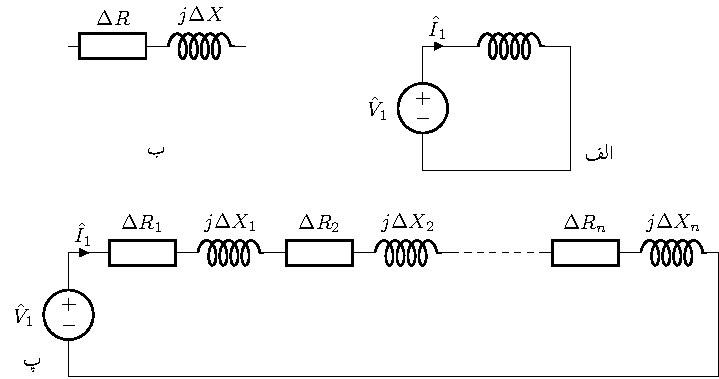
\includegraphics{figTransformersCoilResistanceAndReactance}
\begin{tikzpicture}
%grid
%\draw[gray,thick] (-3,-3) grid (7,3);
%\draw[gray,thin,xstep=0.1,ystep=0.1] (-3,-3) grid (7,3);
%transformer outer dimensions
\pgfmathsetmacro{\h}{2.5}
\begin{scope}[xshift=0cm,yshift=0cm]
\draw(0,0) to [american voltage source,l=$\hat{V}_1$] ++(0,2.1) to  [short,i^=$\hat{I}_1$]  ++(0.5,0) to [inductor,l={لچھا}] ++(2,0) to [short] ++(0,-2.1)--(0,0);
%urdu
\draw (3,0.3) node {الف};
\end{scope}
%
\begin{scope}[xshift=-6cm,yshift=2.1cm]
\draw(0,0) to [european resistor,l=$\Delta R$]  ++(1.5,0) to [inductor,l=$j \Delta X$] ++(1.5,0);
%urdu
\draw (1.5,-1.8) node {ب};
\end{scope}
%
\begin{scope}[xshift=-6cm,yshift=-3.5cm]
\draw(0,0) to [american voltage source,l=$\hat{V}_1$] ++(0,2.1) to  [short,i^=$\hat{I}_1$]  ++(0.5,0) to [european resistor,l=$\Delta R_1$] ++(1.5,0)to [inductor,l=$j\Delta X_1$] ++(1.5,0) to [european resistor,l=$\Delta R_2$] ++(1.5,0)to [inductor,l=$j\Delta X_2$] ++(1.5,0)coordinate(a){};
\draw[dashed](a)--++(1.5,0)coordinate(b){};
 \draw(b) to [european resistor,l=$\Delta R_n$] ++(1.5,0)to [inductor,l=$j\Delta X_n$] ++(1.5,0) to [short] ++(0,-2.1)--(0,0);
%urdu
\draw (-0.6,0.2) node {پ};
\end{scope}
\end{tikzpicture}
\caption{لچھے کی مزاحمت اور متعاملہ۔}
\label{شکل_ٹرانسفارمر_لچھے_کی_مزاحمت_اور_متعاملہ}
\end{figure}

اس دور کی مساوات 
\begin{align*}
\hat{V}_1&=\hat{I}_1 \left(\Delta R_1 + j \Delta X_1 +\Delta R_2 + j \Delta X_2 + \cdots \Delta R_n + j \Delta X_n   \right)\\
&=\hat{I}_1 \left(\Delta R_1 +\Delta R_2 +\cdots \Delta R_n   \right)+\hat{I}_1 \left(j \Delta X_1 + j \Delta X_2+\cdots   j \Delta X_n   \right)
\end{align*}
ہے جس میں
\begin{align*}
R&=\Delta R_1 +\Delta R_2 +\cdots \Delta R_n\\
X&=\Delta X_1 + \Delta X_2 +\cdots   \Delta X_n
\end{align*}
لکھ کر درج ذیل حاصل ہوتا ہے۔
\begin{align}\label{مساوات_ٹرانسفارمر_مزاحمت_علیحدہ}
\hat{V}_1=\hat{I}_1 \left( R +j X \right)
\end{align}
شکل \حوالہ{شکل_ٹرانسفارمر_لچھے_کی_مزاحمت_اور_متعاملہ_کی_علیحدگی}  سے بھی مساوات \حوالہ{مساوات_ٹرانسفارمر_مزاحمت_علیحدہ} لکھی جا سکتی ہے۔ یوں حساب کی خاطر  لچھے کی مزاحمت اور متعاملہ  علیحدہ کیے جا سکتے ہیں۔
\begin{figure}
\centering
%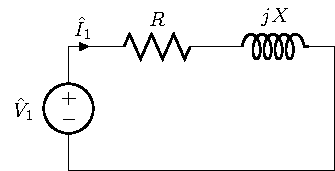
\includegraphics{figTransformersCoilResistanceAndReactanceSeparation}
\begin{tikzpicture}
%grid
%\draw[gray,thick] (-3,-3) grid (7,3);
%\draw[gray,thin,xstep=0.1,ystep=0.1] (-3,-3) grid (7,3);
%transformer outer dimensions
\pgfmathsetmacro{\h}{2.5}
\draw(0,0) to [american voltage source,l=$\hat{V}_1$] ++(0,2.1) to  [short,i^=$\hat{I}_1$]  ++(0.5,0) to [resistor,l=$R$] ++(2,0) to [inductor,l=$j X$] ++(2,0) to [short] ++(0,-2.1)--(0,0);
\end{tikzpicture}
\caption{لچھے کی مزاحمت اور متعاملہ کی علیحدگی۔}
\label{شکل_ٹرانسفارمر_لچھے_کی_مزاحمت_اور_متعاملہ_کی_علیحدگی}
\end{figure}
%
\جزوحصہ{رِستا امالہ}
یہاں تک ہم  کامل ٹرانسفارمر پر بحث کرتے رہے ہیں۔ اب ہم ٹرانسفارمر میں ان عناصر کا ذکر کرتے ہیں جن کی وجہ سے ٹرانسفارمر غیر کامل ہوتا ہے۔ بہت سی جگہوں پر ٹرانسفارمر استعمال کرتے وقت ان عناصر کو مدِ نظر رکھنا ضروری ہوتا ہے۔ ان عناصر کے اثرات کو شامل کرنے کے لئے ہم  ٹرانسفارمر کا مساوی دور بناتے ہیں۔

ابتدائی لچھے کے مقناطیسی بہاو کو دو حصوں میں تقسیم کیا جا سکتا ہے۔ پہلا حصہ وہ جو قالب سے گزر کر ابتدائی اور ثانوی لچھے دونوں کے اندر سے گزرتا ہے۔ یہ مشترکہ مقناطیسی بہاو ہے۔ دوسرا حصہ وہ جو صرف ابتدائی لچھے سے گزرتا ہے اور زیادہ تر قالب کے باہر خلاء میں رہتا ہے۔  اس کو \اصطلاح{رستا  مقناطیسی بہاو}\فرہنگ{مقناطیسی بہاو!رستا}\حاشیہب{leakage magnetic flux}\فرہنگ{magnetic flux!leakage}   کہتے ہیں۔چونکہ ہوا کا مقناطیسی مستقل \عددیء{\mu_0} اٹل ہے لہٰذا یہاں ہچکچاہٹ بھی اٹل ہو گی۔  یوں رستا مقناطیسی بہاو ابتدائی لچھے کے برقی رو کا  راست متناسب ہو گا۔

رستا امالہ کے اثر کو بالکل لچھے کی مزاحمت کی طرح لچھے سے باہر \اصطلاح{رستا امالہ}\فرہنگ{رستا!امالہ}\حاشیہب{leakage inductance}\فرہنگ{leakage inductance} \عددیء{L_1} یا \اصطلاح{رستا متعاملہ}\فرہنگ{رستا!متعاملہ}\حاشیہب{leakage reactance}\فرہنگ{leakage reactance}  \عددیء{X_1=2\pi f L_1} سے ظاہر کیا جاتا ہے۔

ٹرانسفارمر کے ابتدائی لچھے میں برقی رو \عددیء{\hat{I_1}}  گزرنے سے رستا متعاملہ میں \عددیء{\hat{V}_{X1}=j \hat{I}_1 X_1} برقی دباو اور لچھے کے تار کی مزاحمت  میں \عددیء{\hat{V}_{R1}=\hat{I}_1 R_1} برقی دباو گھٹتا ہے۔

جیسا شکل \حوالہ{شکل_ٹرانسفارمر_ماڈل_حصہ_اول}  میں دکھایا گیا ہے، ابتدائی لچھے  پر لاگو دباو \عددیء{\hat{V}_1}،   مزاحمت \عددیء{R_1} اور متعاملہ   \عددیء{X_1} میں گھٹاو اور  ابتدائی امالی دباو \عددیء{\hat{E}_1} کا مجموعہ  ہو گا۔  
\begin{figure}
\centering
%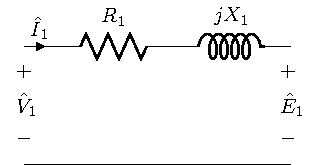
\includegraphics{figTransformersModelFirstPart}
\begin{tikzpicture}
%grid
%\draw[gray,thick] (-3,-3) grid (5,3);
%\draw[gray,thin,xstep=0.1,ystep=0.1] (-3,-3) grid (5,3);
%transformer outer dimensions
\pgfmathsetmacro{\h}{2.5}
\draw(0,0)  to  [short,i^=$\hat{I}_1$]  ++(0.5,0) to [resistor,l=$R_1$] ++(2,0) to [inductor,l=$j X_1$] ++(2,0); 
\draw(0,-2) to ++(4.5,0);
\draw(0,-1) node{$
\begin{aligned}
&+\\
&\hat{V}_1\\
&-
\end{aligned}
$};
%
\draw(4.5,-1) node{$
\begin{aligned}
&+\\
&\hat{E}_1\\
&-
\end{aligned}
$};
\end{tikzpicture}
\caption{ٹرانسفارمر مساوی دور، حصہ اول۔}
\label{شکل_ٹرانسفارمر_ماڈل_حصہ_اول}
\end{figure}
%

\جزوحصہ{ثانوی برقی رو اور قالب کے اثرات}
قالب میں دونوں لچھوں کا مشترکہ مقناطیسی بہاو ان کے مجموعی مقناطیسی دباو کی وجہ سے وجود میں آتا ہے۔ اس حقیقت  کو ایک مختلف اور بہتر انداز میں بیان کیا جا سکتا ہے۔ ہم کہتے ہیں کہ ابتدائی برقی رو کو دو شرائط مطمئن کرنے ہوں گے۔ اول اسے قالب میں ہیجانی مقناطیسی بہاو وجود میں لانا ہو گا اور دوم اسے ثانوی لچھے کے پیدا کردہ مقناطیسی بہاو کو ختم کرنا ہو گا۔ لہٰذا ابتدائی برقی رو کو ہم دو حصوں میں تقسیم کر سکتے ہیں۔ ایک حصہ \عددیء{i_{\varphi}} جو ہیجانی مقناطیسی بہاو پیدا کرتا ہے اور دوسرا \عددیء{\hat{I}_2'} جو ثانوی لچھے کے مقناطیسی دباو کا اثر  ختم کرتا ہے۔یوں \عددی{\hat{I_2'}} درج ذیل ہو گا۔
\begin{align}
\hat{I}_2'=\frac{N_2}{N_1} \hat{I}_2
\end{align}
 ثانوی لچھے کے مقناطیسی بہاو کے اثر کو ختم کرنے پر حصہ \حوالہ{حصہ_ٹرانسفارمر_ثانوی_بار_کا_ابتدائی_جانب_اثر}  میں غور کیا گیا ہے۔

 اگرچہ برقی رو \عددیء{i_{\varphi}} غیر سائن نما ہوتا ہے ہم  اسے سائن نما \عددیء{\hat{I}_\varphi}  تصور  کر کے  دو حصوں، \عددی{\hat{I}_c} اور \عددی{\hat{I}_m}، میں تقسیم کرتے ہیں۔
\begin{align}\label{مساوات_ٹرانسفارمر_رو_ہیجان_ضیاع_اجزاع}
\hat{I}_\varphi=\hat{I}_c+\hat{I}_m
\end{align}
مذکورہ بالا مساوات میں برقی رو کو مرحلی سمتیات کی صورت میں لکھا گیا ہے۔ان میں \عددیء{\hat{I}_c}  ابتدائی لچھے کے امالی برقی دباو \عددیء{\hat{E}_1} کا ہم قدم ہے اور  قالب میں برقی توانائی کے ضیاع کو ظاہر کرتا ہے جبکہ \عددیء{\hat{I}_m}  وہ حصہ ہے جو \عددیء{\hat{E}_1} سے نوے درجہ زاویہ \اصطلاح{پیچھے}\فرہنگ{پیچھے}\حاشیہب{lagging}  رہتا اور  لچھے میں مقناطیسی بہاو پیدا کرتا ہے۔

شکل \حوالہ{شکل_ٹرانسفارمر_ماڈل_حصہ_دوم} میں \عددیء{R_c}  اور  \عددیء{j X_m} بالترتیب برقی رو \عددی{\hat{I}_c} اور \عددی{\hat{I}_m} کے اثرات کو ظاہر کرنے کے لئے استعمال کیے گئے ہیں۔مزاحمت \عددیء{R_c} کی مقدار اتنی رکھی جاتی ہے کہ اس میں برقی طاقت کا ضیاع اصل قالبی ضیاع کے برابر ہو یعنی \عددیء{p_c=E_{1,rms}^2/R_c}۔یوں  \عددی{R_c=E_{1,rms}^2/p_c} ہو گا۔ اسی طرح \عددیء{j X_m} کی مقدار اتنی رکھی جاتی ہے کہ \عددیء{\hat{I}_m=\hat{E}_1/jX_{m}} ہو۔ \عددیء{R_c} اور \عددیء{j X_m}  کی مقدار اصل برقی دباو اور تعدد پر حاصل کئے جاتے ہیں۔ 

\begin{figure}
\centering
%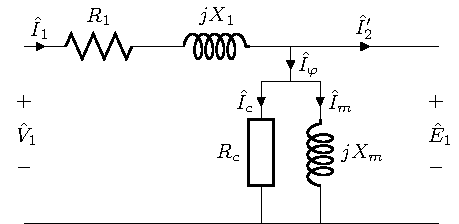
\includegraphics{figTransformersModelSecondPart}
\begin{tikzpicture}
%grid
%\draw[gray,thick] (-3,-3) grid (7,1);
%\draw[gray,thin,xstep=0.1,ystep=0.1] (-3,-3) grid (7,1);
%transformer outer dimensions
\pgfmathsetmacro{\h}{2.5}
\def\ky{-3};
\draw(0,0)  to  [short,i^=$\hat{I}_1$]  ++(0.5,0) to [resistor,l=$R_1$] ++(1.5,0) to [inductor,l=$j X_1$] ++(2.5,0)coordinate(a){} to [short,i=$\hat{I}_2'$] ++(2.5,0); 
\draw(0,\ky) to ++(7,0);
\draw(a) to [short,i=$\hat{I}_\varphi$,*-*] ++(0,-0.6);
\draw(4,-0.6) to [short] ++(1,0);
\draw(4,\ky) to [european resistor,l=$R_c$,i^<=$\hat{I}_c$,*-] ++(0,2.4);
\draw(5,\ky) to [inductor,l_=$j X_m$,i_<=$\hat{I}_m$,*-] ++(0,2.4);
%
\draw(0,\ky/2) node{$
\begin{aligned}
&+\\
&\hat{V}_1\\
&-
\end{aligned}
$};
%
\draw(7,\ky/2) node{$
\begin{aligned}
&+\\
&\hat{E}_1\\
&-
\end{aligned}
$};
\end{tikzpicture}
\caption{ٹرانسفارمر مساوی دور، حصہ دوم۔}
\label{شکل_ٹرانسفارمر_ماڈل_حصہ_دوم}
\end{figure}

\جزوحصہ{ثانوی لچھے کا امالی برقی دباو}
قالب میں مشترکہ مقناطیسی بہاو ثانوی لچھے میں امالی برقی دباو \عددیء{\hat{E}_2} پیدا کرے گا۔ چونکہ یہی مقناطیسی بہاو ابتدائی لچھے میں \عددیء{\hat{E}_1}  امالی پیدا کرتا ہے لہٰذا درج ذیل لکھا جا سکتا ہے۔
\begin{align}\label{مساوات_ٹرانسفارمر_دباو_رو_شرح}
\frac{\hat{E}_1}{\hat{E}_2}=\frac{N_1}{N_2}
\end{align}
مساوات \حوالہ{مساوات_ٹرانسفارمر_رو_ہیجان_ضیاع_اجزاع} اور مساوات \حوالہ{مساوات_ٹرانسفارمر_دباو_رو_شرح}  کو ایک کامل ٹرانسفارمر سے ظاہر کیا جا سکتا ہے جسے  شکل \حوالہ{شکل_ٹرانسفارمر_ماڈل_حصہ_ثوم}  میں دکھایا گیا ہے۔
\begin{figure}
\centering
%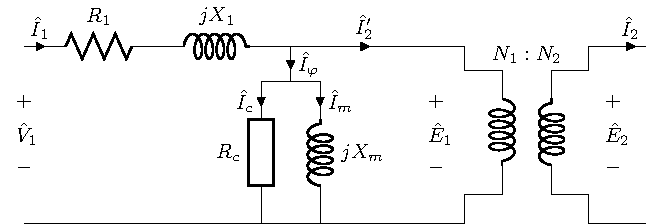
\includegraphics{figTransformersModelThirdPart}
\begin{tikzpicture}
%grid
%\draw[gray,thick] (0,-3) grid (9,1);
%\draw[gray,thin,xstep=0.1,ystep=0.1] (0,-3) grid (9,1);
%transformer outer dimensions
\pgfmathsetmacro{\h}{2.5}
\def\ky{-3};
\draw(0,0)  to  [short,i^=$\hat{I}_1$]  ++(0.5,0) to [resistor,l=$R_1$] ++(1.5,0) to [inductor,l=$j X_1$] ++(2.5,0)coordinate(a){} to [short,i=$\hat{I}_2'$] ++(2.5,0); 
\draw(0,\ky) to ++(7,0);
\draw(a) to [short,i=$\hat{I}_\varphi$,*-*] ++(0,-0.6);
\draw(4,-0.6) to [short] ++(1,0);
\draw(4,\ky) to [european resistor,l=$R_c$,i^<=$\hat{I}_c$,*-] ++(0,2.4);
\draw(5,\ky) to [inductor,l_=$j X_m$,i_<=$\hat{I}_m$,*-] ++(0,2.4);
%
\draw(0,\ky/2) node{$
\begin{aligned}
&+\\
&\hat{V}_1\\
&-
\end{aligned}
$};
%
\draw(7,\ky/2) node{$
\begin{aligned}
&+\\
&\hat{E}_1\\
&-
\end{aligned}
$};
%transformer
\draw (8.5,-0.4) node[transformer](T){};
\draw(T.A1) |- (7,0);
\draw(T.A2) |- (7,-3);
\draw(T.B1) |- (10,0) to [short,i=$\hat{I}_2$] ++(0.5,0);
\draw(T.B2) |- (10,\ky) to [short] ++(0.5,0);
%
\draw(10,\ky/2) node{$
\begin{aligned}
&+\\
&\hat{E}_2\\
&-
\end{aligned}
$};
\draw(T.base) node[above]{$N_1:N_2$};
\end{tikzpicture}
\caption{ٹرانسفارمر مساوی دور، حصہ ثوم۔}
\label{شکل_ٹرانسفارمر_ماڈل_حصہ_ثوم}
\end{figure}

\جزوحصہ{ثانوی لچھے کی مزاحمت اور متعاملہ کے اثرات}
ثانوی لچھے میں امالی دباو \عددیء{\hat{E}_2}پیدا ہو گا۔ابتدائی لچھے کی طرح، ثانوی لچھے کی مزاحمت \عددیء{R_2}  اور متعاملہ  \عددیء{j X_2} ہوں گے جن میں ثانوی برقی رو \عددیء{\hat{I}_2}  کی بنا برقی دباو گھٹے گا۔ یوں ثانوی لچھے کے سروں پر برقی دباو \عددی{\hat{V}_2} قدرِ کم ہو گا:
\begin{align}
\hat{V}_2=\hat{E}_2-\hat{I}_2 R_2-j \hat{I}_2 X_2
\end{align}
یوں حاصل ٹرانسفارمر کا مکمل مساوی دور یا \اصطلاح{ریاضی نمونہ}\فرہنگ{ریاضی نمونہ}\حاشیہب{mathematical model}\فرہنگ{model} شکل  \حوالہ{شکل_ٹرانسفارمر_مکمل_ماڈل} میں دکھایا گیا ہے۔
\begin{figure}
\centering
%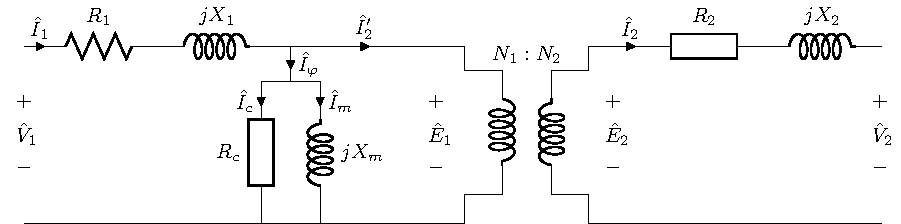
\includegraphics[width=0.9\linewidth]{figTransformersModelComplete}
\begin{tikzpicture}[xscale=0.75]
%grid
%\draw[gray,thick] (0,-3) grid (15,1);
%\draw[gray,thin,xstep=0.1,ystep=0.1] (0,-3) grid (15,1);
%transformer outer dimensions
\pgfmathsetmacro{\h}{2.5}
\def\ky{-3};
\draw(0,0)  to  [short,i^=$\hat{I}_1$]  ++(0.5,0) to [resistor,l=$R_1$] ++(1.5,0) to [inductor,l=$j X_1$] ++(2.5,0)coordinate(a){} to [short,i=$\hat{I}_2'$] ++(2.5,0); 
\draw(0,\ky) to ++(7,0);
\draw(a) to [short,i=$\hat{I}_\varphi$,*-*] ++(0,-0.6);
\draw(4,-0.6) to [short] ++(1,0);
\draw(4,\ky) to [european resistor,l=$R_c$,i^<=$\hat{I}_c$,*-] ++(0,2.4);
\draw(5,\ky) to [inductor,l_=$j X_m$,i_<=$\hat{I}_m$,*-] ++(0,2.4);
%
\draw(0,\ky/2) node{$
\begin{aligned}
&+\\
&\hat{V}_1\\
&-
\end{aligned}
$};
%
\draw(7,\ky/2) node{$
\begin{aligned}
&+\\
&\hat{E}_1\\
&-
\end{aligned}
$};
%transformer
\draw (8.5,-0.4) node[transformer](T){};
\draw(T.base) node[above]{$N_1:N_2$};
\draw(T.A1) |- (7,0);
\draw(T.A2) |- (7,-3);
\draw(T.B1) |- (10,0) to [short,i=$\hat{I}_2$] ++(0.5,0) to [european resistor,l=$R_2$] ++(2,0) to [inductor,l=$j X_2$] ++(2,0);
\draw(T.B2) |- (10,\ky) to [short] ++(4.5,0);
%
\draw(10,\ky/2) node{$
\begin{aligned}
&+\\
&\hat{E}_2\\
&-
\end{aligned}
$};
%
\draw(14.5,\ky/2) node{$
\begin{aligned}
&+\\
&\hat{V}_2\\
&-
\end{aligned}
$};
\end{tikzpicture}
\caption{ٹرانسفارمر کا مکمل مساوی دور یا ریاضی نمونہ۔}
\label{شکل_ٹرانسفارمر_مکمل_ماڈل}
\end{figure}

%%%%%%%%%%%%%%%%%%%%%%%%%%%%%%%%%%%%%%%%

\جزوحصہ{رکاوٹ کا ابتدائی یا ثانوی جانب تبادلہ}
شکل \حوالہ{شکل_ٹرانسفارمر_مکمل_ماڈل}  میں دکھائے دور کے سب جزو کا تبادلہ ایک جانب سے دوسری جانب کیا جا سکتا ہے۔ یہ کرنے سے کامل ٹرانسفارمر کو مساوی دور کی بائیں یا دائیں جانب لے جایا جا سکتا ہے۔شکل \حوالہ{شکل_ٹرانسفارمر_مکمل_ماڈل_ابتدائی_جانب}   میں ثانوی جانب کی رکاوٹ کا ابتدائی جانب تبادلہ کیا گیا ہے جبکہ شکل  \حوالہ{شکل_ٹرانسفارمر_مکمل_ماڈل_ثانوی_جانب}  میں ابتدائی جانب کی رکاوٹ کا ثانوی جانب تبادلہ کیا گیا ہے۔اس طرح حاصل مساوی دور میں عموماً کامل ٹرانسفارمر بنایا ہی نہیں جاتا۔یہی شکل \حوالہ{شکل_ٹرانسفارمر_مکمل_ماڈل_ثانوی_جانب}   میں کیا گیا ہے۔

تبادلہ شدہ رکاوٹ  \عددیء{Z} کو \عددیء{Z'}  سے ظاہر کیا جاتا ہے۔یوں \عددیء{R_2} کے ٹرانسفارمر کی دوسری جانب تبادلہ کے بعد اسے \عددیء{R_2'} سے ظاہر کیا گیا ہے۔

ایسا دور استعمال کرتے وقت یہ ذہن میں رکھنا ہوتا ہے کہ ٹرانسفارمر کے کس جانب دور حل کیا جا رہا ہے۔
\begin{figure}
\centering
%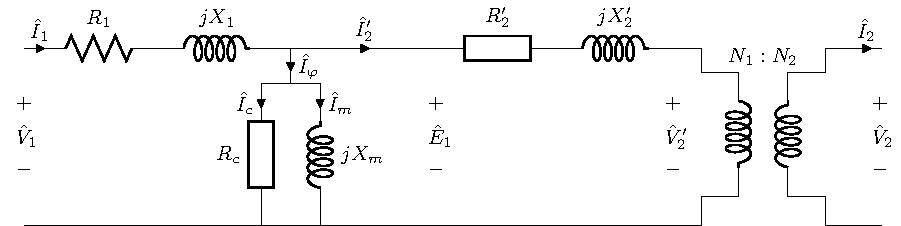
\includegraphics[width=0.9\linewidth]{figTransformersModelShiftedToPrimarySide}
\begin{tikzpicture}[xscale=0.75]
%grid
%\draw[gray,thick] (0,-4) grid (15,1);
%\draw[gray,thin,xstep=0.1,ystep=0.1] (0,-4) grid (15,1);

%transformer outer dimensions
\pgfmathsetmacro{\h}{2.5}
\def\ky{-3};
\draw(0,0)  to  [short,i^=$\hat{I}_1$]  ++(0.5,0) to [resistor,l=$R_1$] ++(1.5,0) to [inductor,l=$j X_1$] ++(2.5,0)coordinate(a){} to [short,i=$\hat{I}_2'$] ++(2.5,0) to
[european resistor,l=$R_2'$] ++(2,0) to [inductor,l=$j X_2'$] ++(2,0); 
%\draw(0,\ky) to [short]++(11,0);
\draw(a) to [short,i=$\hat{I}_\varphi$,*-*] ++(0,-0.6);
\draw(4,-0.6) to [short] ++(1,0);
\draw(4,\ky) to [european resistor,l=$R_c$,i^<=$\hat{I}_c$,*-] ++(0,2.4);
\draw(5,\ky) to [inductor,l_=$j X_m$,i_<=$\hat{I}_m$,*-] ++(0,2.4);
%
\draw(0,\ky/2) node{$
\begin{aligned}
&+\\
&\hat{V}_1\\
&-
\end{aligned}
$};
%
\draw(7,\ky/2) node{$
\begin{aligned}
&+\\
&\hat{E}_1\\
&-
\end{aligned}
$};
%transformer
\draw (12.5,-0.4) node[transformer](T){};
\draw(T.base) node[above]{$N_1:N_2$};
\draw(T.A1) |- (11,0);
\draw(T.A2) |- (0,-3);
\draw(T.B1) |- (14,0) to [short,i=$\hat{I}_2$] ++(0.5,0);
\draw(T.B2) |- (14,\ky) to [short] ++(0.5,0);
%
\draw(11,\ky/2) node{$
\begin{aligned}
&+\\
&\hat{V}_2'\\
&-
\end{aligned}
$};
%
\draw(14.5,\ky/2) node{$
\begin{aligned}
&+\\
&\hat{V}_2\\
&-
\end{aligned}
$};
\end{tikzpicture}
\caption{ثانوی جانب رکاوٹ کا ابتدائی جانب تبادلہ کیا گیا ہے۔}
\label{شکل_ٹرانسفارمر_مکمل_ماڈل_ابتدائی_جانب}
\end{figure}
%
\begin{figure}
\centering
%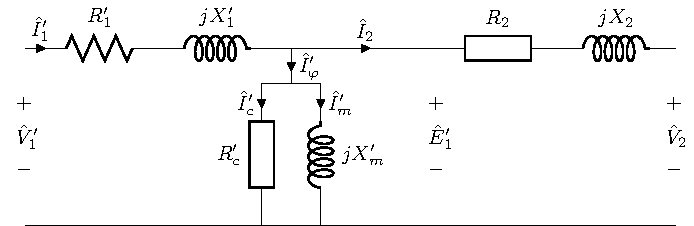
\includegraphics[width=0.9\linewidth]{figTransformersModelShiftedToSecondarySide}
\begin{tikzpicture}[xscale=0.75]
%grid
%\draw[gray,thick] (0,-4) grid (15,1);
%\draw[gray,thin,xstep=0.1,ystep=0.1] (0,-4) grid (15,1);
%transformer outer dimensions
\pgfmathsetmacro{\h}{2.5}
\def\ky{-3};
\draw(0,0)  to  [short,i^=$\hat{I}_1'$]  ++(0.5,0) to [resistor,l=$R_1'$] ++(1.5,0) to [inductor,l=$j X_1'$] ++(2.5,0)coordinate(a){} to [short,i=$\hat{I}_2$] ++(2.5,0) to
[european resistor,l=$R_2$] ++(2,0) to [inductor,l=$j X_2$] ++(2,0); 
\draw(0,\ky) to [short]++(11,0);
\draw(a) to [short,i=$\hat{I}_\varphi'$,*-*] ++(0,-0.6);
\draw(4,-0.6) to [short] ++(1,0);
\draw(4,\ky) to [european resistor,l=$R_c'$,i^<=$\hat{I}_c'$,*-] ++(0,2.4);
\draw(5,\ky) to [inductor,l_=$j X_m'$,i_<=$\hat{I}_m'$,*-] ++(0,2.4);
%
\draw(0,\ky/2) node{$
\begin{aligned}
&+\\
&\hat{V}_1'\\
&-
\end{aligned}
$};
%
\draw(7,\ky/2) node{$
\begin{aligned}
&+\\
&\hat{E}_1'\\
&-
\end{aligned}
$};
%
\draw(11,\ky/2) node{$
\begin{aligned}
&+\\
&\hat{V}_2\\
&-
\end{aligned}
$};
%
\end{tikzpicture}
\caption{ابتدائی جانب رکاوٹ کا ثانوی جانب تبادلہ کیا گیا ہے۔}
\label{شکل_ٹرانسفارمر_مکمل_ماڈل_ثانوی_جانب}
\end{figure}


%
\ابتدا{مثال}
ایک \عددیء{50} کلو وولٹ-ایمپیئر اور  \عددیء{2200:220} وولٹ برقی سکت کے ٹرانسفارمر کی زیادہ برقی دباو کی جانب کی رستا رکاوٹ \عددیء{Z_1=0.9+j 1.2}  اوہم اور کم برقی دباو کی جانب کی رِستا رکاوٹ \عددیء{Z_2=0.0089+j 0.011} اوہم ہے۔اگر اس کی \عددیء{R_c=\SI{6.4}{\kilo\ohm}} اور \عددیء{X_m=\SI{47}{\kilo\ohm}}  ہو تو اس کی شکل \حوالہ{شکل_ٹرانسفارمر_مکمل_ماڈل_ابتدائی_جانب}  اور شکل \حوالہ{شکل_ٹرانسفارمر_مکمل_ماڈل_ثانوی_جانب}  میں استعمال ہونے والے جزو معلوم کریں۔

	حل حصہ اول:
معلومات:
\begin{align*}
\SI{50}{\kilo \volt \ampere}, \quad \SI{50}{\hertz}, \quad 2200:220\,\textup{V}
\end{align*}
ٹرانسفارمر کے دونوں جانب کی برقی دباو لچھوں کے چکروں کی نسبت سے ہوتے ہیں لہٰذا
\begin{align*}
\frac{N_1}{N_2}=\frac{2200}{220}=\frac{10}{1}
\end{align*}
یوں اگر ٹرانسفارمر کی رکاوٹ کا زیادہ برقی دباو کی جانب تبادلہ کیا جائے تو
\begin{align*}
R_2'+j X_2' &=\left(\frac{N_1}{N_2} \right)^2 \left(R_2+j X_2 \right)\\
&=\left(\frac{10}{1} \right)^2 \left(0.0089+j 0.011 \right)\\
&=0.89+j 1.1
\end{align*}
جبکہ اس کی بقایا رکاوٹ وہی رہیں گے۔یوں شکل \حوالہ{شکل_ٹرانسفارمر_مکمل_ماڈل_ابتدائی_جانب}  کے جزو حاصل ہوئے۔

	حل حصہ دوم:
اگر مساوی دور کی رکاوٹ کا کم برقی دباو کی جانب تبادلہ کیا جائے تب
\begin{align*}
R_1'+j X_1' &=\left(\frac{N_2}{N_1} \right)^2 \left(R_1+j X_1 \right)\\
&=\left(\frac{1}{10} \right)^2 \left(0.9+j1.2 \right)\\
&=0.009+j0.012
\end{align*}
اسی طرح
\begin{align*}
R_c'&=\left(\frac{N_2}{N_1} \right)^2 R_c=64\\
X_m'&=\left(\frac{N_2}{N_1} \right)^2 X_m=470
\end{align*}
جبکہ \عددیء{Z_2} وہی رہے گا۔
\انتہا{مثال}
%
\جزوحصہ{ٹرانسفارمر کے سادہ ترین مساوی دور}
ایک انجنیئر کو جب ایک ٹرانسفارمر استعمال کرنا ہو تو وہ حساب کرتے وقت شکل \حوالہ{شکل_ٹرانسفارمر_مکمل_ماڈل_ابتدائی_جانب}  میں دیئے گئے دور کو استعمال کر سکتا ہے۔ یہ دور حقیقی ٹرانسفارمر کی بہت اچھی عکاسی کرتا ہے۔ البتہ جہاں ہمیں نہایت صحیح جواب مطلوب نہ ہوں وہاں اس دور کی سادہ اشکال بھی استعمال کی جا سکتیں ہیں۔ اس باب میں ہم ایسے ہی سادہ مساوی دوروں کا ذکر کریں گے۔
\begin{figure}
\centering
%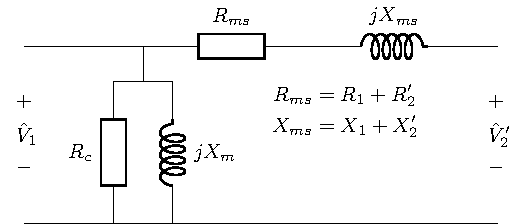
\includegraphics[width=0.9\linewidth]{figTransformersModelLeftHand}
\begin{tikzpicture}
%grid
%\draw[gray,thick] (0,-4) grid (8,1);
%\draw[gray,thin,xstep=0.1,ystep=0.1] (0,-4) grid (8,1);
%transformer outer dimensions
\pgfmathsetmacro{\h}{2.5}
\def\ky{-3};
\draw(0,0)  to  [short]  ++(2.5,0)  to [european resistor,l=$R_{ms}$] ++(2,0) to [inductor,l=$j X_{ms}$] ++(3.5,0); 
\draw(0,\ky) to [short]++(8,0);
\draw(2,0) to [short,*-*] ++(0,-0.6);
\draw(1.5,-0.6) to [short] ++(1,0);
\draw(1.5,\ky) to [european resistor,l=$R_c$,*-] ++(0,2.4);
\draw(2.5,\ky) to [inductor,l_=$j X_m$,*-] ++(0,2.4);
%
\draw(0,\ky/2) node{$
\begin{aligned}
&+\\
&\hat{V}_1\\
&-
\end{aligned}
$};
%
\draw(8,\ky/2) node{$
\begin{aligned}
&+\\
&\hat{V}_2'\\
&-
\end{aligned}
$};
%
\draw(4,-0.5)node[below right]{$
\begin{aligned}
R_{ms}&=R_1+R_2'\\
X_{ms}&=X_1+X_2'
\end{aligned}
$};
\end{tikzpicture}
\caption{\عددیء{R_c} اور \عددیء{jX_m} کو بائیں جانب منتقل کیا گیا ہے۔}
\label{شکل_ٹرانسفارمر_بائیں_جانب}
\end{figure}
%
\begin{figure}
\centering
%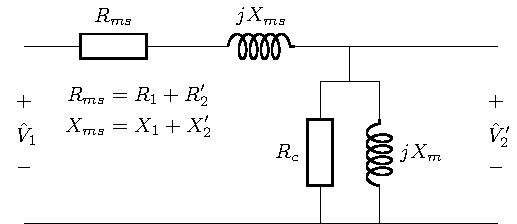
\includegraphics[width=0.9\linewidth]{figTransformersModelRightHand}
\begin{tikzpicture}
%grid
%\draw[gray,thick] (0,-4) grid (8,1);
%\draw[gray,thin,xstep=0.1,ystep=0.1] (0,-4) grid (8,1);
%transformer outer dimensions
\pgfmathsetmacro{\h}{2.5}
\def\ky{-3};
\draw(0,0)  to  [short]  ++(0.5,0)  to [european resistor,l=$R_{ms}$] ++(2,0) to [inductor,l=$j X_{ms}$] ++(3,0) to [short] ++(2.5,0); 
\draw(0,\ky) to [short]++(8,0);
\draw(5.5,0) to [short,*-*] ++(0,-0.6);
\draw(5,-0.6) to [short] ++(1,0);
\draw(5,\ky) to [european resistor,l=$R_c$,*-] ++(0,2.4);
\draw(6,\ky) to [inductor,l_=$j X_m$,*-] ++(0,2.4);
%
\draw(0,\ky/2) node{$
\begin{aligned}
&+\\
&\hat{V}_1\\
&-
\end{aligned}
$};
%
\draw(8,\ky/2) node{$
\begin{aligned}
&+\\
&\hat{V}_2'\\
&-
\end{aligned}
$};
%
\draw(0.5,-0.5)node[below right]{$
\begin{aligned}
R_{ms}&=R_1+R_2'\\
X_{ms}&=X_1+X_2'
\end{aligned}
$};
\end{tikzpicture}
\caption{\عددیء{R_c} اور \عددیء{jX_m} کو دائیں جانب منتقل کیا گیا ہے۔}
\label{شکل_ٹرانسفارمر_دائیں_جانب}
\end{figure}

شکل  \حوالہ{شکل_ٹرانسفارمر_مکمل_ماڈل_ابتدائی_جانب} میں \عددیء{R_c} اور \عددیء{X_m} کو بائیں یا دائیں طرف لے جانے سے  شکل  \حوالہ{شکل_ٹرانسفارمر_بائیں_جانب}  اور  شکل \حوالہ{شکل_ٹرانسفارمر_دائیں_جانب}  حاصل ہوتے ہیں۔چونکہ \عددیء{\hat{I}_\varphi} کی مقدار نہایت کم\حاشیہد{\عددیء{\hat{I}_\varphi} ٹرانسفارمر کے کل برقی بوجھ کے صرف دو سے چھ فی صد ہوتی ہے}  ہوتی ہے اس لئے ایسا  کرنے سے حاصل جواب پر کوئی خاص فرق نہیں پڑتا۔ چونکہ اس شکل میں \عددیء{R_1} ،\عددیء{R_2'}، \عددیء{X_1}  اور \عددیء{X_2'} سلسلہ وار ہیں اس لئے ان کو جمع کیا جا سکتا ہے شکل میں ان کو مساوی مزاحمت \عددیء{R_{ms}}  اور مساوی متعاملہ \عددیء{X_{ms}} کہا گیا ہے۔اسی قسم کے ادوار  شکل  \حوالہ{شکل_ٹرانسفارمر_مکمل_ماڈل_ثانوی_جانب} سے بھی حاصل ہوتے  ہیں۔

ہم ایک قدم اور آگے جا سکتے ہیں اور \عددیء{\hat{I}_\varphi} کو مکمل طور پر نظر انداز کر سکتے ہیں یعنی اس کو ہم صفر تصور کر لیتے ہیں۔اس کا مطلب ہے کہ مساوی دور میں \عددیء{R_c} اور \عددیء{j X_m} دونوں کو کھلے دور کیا جاتا ہے  یعنی انہیں مساوی دور سے ہٹا دیا جاتا ہے۔ شکل \حوالہ{شکل_ٹرانسفارمر_سادہ_ماڈل}-الف  میں ایسا کیا گیا ہے۔اس دور میں قالب کے اثرات کو مکمل طور پر نظرانداز کیا گیا ہے۔

بیشتر وقت ہمیں اس سے بھی کم صحیح جواب مطلوب ہوتا ہے۔چونکہ \عددیء{X_m\gg R_c}  لہٰذا ہم  \عددیء{R_{ms}} کو بھی نظرانداز کر سکتے ہیں۔یوں شکل \حوالہ{شکل_ٹرانسفارمر_سادہ_ماڈل}-ب حاصل ہوتا ہے۔
\begin{figure}
\centering
%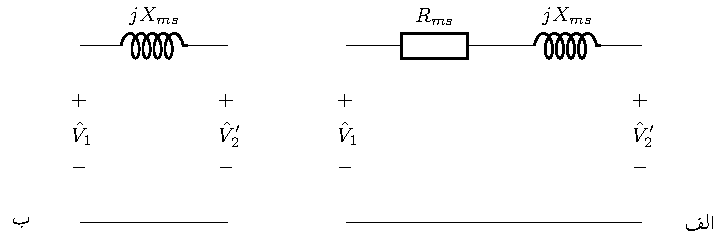
\includegraphics[width=0.9\linewidth]{figTransformersModelCoreLossNeglected}
\begin{tikzpicture}
%grid
%\draw[gray,thick] (0,-4) grid (8,1);
%\draw[gray,thin,xstep=0.1,ystep=0.1] (0,-4) grid (8,1);
%transformer outer dimensions
\pgfmathsetmacro{\h}{2.5}
\def\ky{-3};
\begin{scope}[xshift=4.5cm]
\draw(0,0)  to  [short]  ++(0.5,0)  to [european resistor,l=$R_{ms}$] ++(2,0) to [inductor,l=$j X_{ms}$] ++(2.5,0); 
\draw(0,\ky) to [short]++(5,0);
%
\draw(0,\ky/2) node{$
\begin{aligned}
&+\\
&\hat{V}_1\\
&-
\end{aligned}
$};
%
\draw(5,\ky/2) node{$
\begin{aligned}
&+\\
&\hat{V}_2'\\
&-
\end{aligned}
$};
%
\draw(6,\ky) node{الف};
\end{scope}
%
\draw(0,0)   to [inductor,l=$j X_{ms}$] ++(2.5,0); 
\draw(0,\ky) to [short]++(2.5,0);
%
\draw(0,\ky/2) node{$
\begin{aligned}
&+\\
&\hat{V}_1\\
&-
\end{aligned}
$};
%
\draw(2.5,\ky/2) node{$
\begin{aligned}
&+\\
&\hat{V}_2'\\
&-
\end{aligned}
$};
%
\draw(-1,\ky) node{ب};
\end{tikzpicture}
\caption{ٹرانسفارمر کے سادہ مساوی ادوار۔}
\label{شکل_ٹرانسفارمر_سادہ_ماڈل}
\end{figure}
\حصہ{کھلے دور معائنہ اور کسرِ دور معائنہ}
پچھلے حصے میں بیان کئے گئے ٹرانسفارمر کے مساوی دور کے جزو ٹرانسفارمر کے دو معائنوں سے حاصل کئے جا سکتے ہیں۔ ان معائنوں کو کھلے دور معائنہ اور کسرِ دور معائنہ کہتے ہیں۔اس حصے میں انہیں پر غور کیا جائے گا۔

\جزوحصہ{کھلے دور معائنہ}
کھلے  دور معائنہ\فرہنگ{معائنہ!کھلے دور}\حاشیہب{open circuit test}\فرہنگ{open circuit test} جیسا کہ نام سے واضح  ہے،  ٹرانسفارمر کی ایک جانب لچھے کے سروں کو آزاد رکھ کر کیا جاتا ہے۔ یہ معائنہ اتنی برقی دباو اور تعدد یا ان کے قریب ترین مقداروں پر کیا جاتا ہے جتنے پر ٹرانسفارمر کی بناوٹ\فرہنگ{بناوٹ}\حاشیہب{design} ہو۔ اگرچہ یہ معائنہ ٹرانسفارمر کے کسی بھی جانب کے لچھے پر کیا جا سکتا ہے، حقیقت میں اسے کم برقی دباو والی جانب کے لچھے پر کرنا آسان ہوتا ہے۔یہ بات ایک مثال سے زیادہ آسانی سے سمجھ آتی ہے۔

	مثلاً  ہم  \عددیء{\SI{25}{\kilo \volt \ampere}} اور \عددیء{11000:220\,\textup{V}}  کا \عددیء{\SI{50}{\hertz}} پر چلنے والے ایک دور کے ٹرانسفارمر کا معائنہ کرنا چاہتے ہیں۔ اگر یہ معائنہ اس کے گیارہ ہزار کے لچھے پر  کیا جائے تو گیارہ ہزار برقی دباو کے لگ بھگ برقی دباو استعمال کیا جائے گا اور اگر دو سو بیس برقی دباو والے لچھے پر کیا جائے تو دو سو بیس برقی دباو کے لگ بھگ برقی دباو  استعمال کیا جائے گا۔ دونوں صورتوں میں تعدد \عددیء{\SI{50}{\hertz}} کے لگ بھگ رکھا جائے گی۔\عددیء{\SI{11}{\kilo \volt}} کی برقی دباو پر کام کرنا نہایت خطرناک ثابت ہو سکتا ہے۔یہی وجہ ہے کہ اس معائنہ کو کم برقی دباو والے لچھے پر ہی کیا جاتا ہے۔

 جس برقی دباو پر ٹرانسفارمر عام حالات میں استعمال ہوتا ہے اس معائنہ میں کم برقی دباو والی جانب کے لچھے پر اتنے ہی یا اس کی قریب مقدار کی برقی دباو \عددیء{V_t} لاگو کر کے کھلے دور برقی طاقت \عددیء{p_t} اور  کھلے دور برقی رو \عددیء{I_t}  ناپے جاتے ہیں۔معائنہ حقیقت میں استعمال کے دوران برقی دباو کے جتنے قریب برقی دباو پر کیا جائے اتنا بہتر جواب حاصل ہوتا ہے۔ ٹرانسفارمر کی دوسری جانب لچھے کے سرے چونکہ آزاد رکھے جاتے ہیں اس لئے اس میں  برقی رو صفر ہو گا۔  لہٰذا ناپا گیا برقی رو صرف ہیجان انگیز برقی رو \عددیء{\hat{I}_\varphi} ہو گا۔ ٹرانسفارمر جتنی برقی رو کے لئے بنایا گیا ہو یہ برقی رو اس  کے تقریباً دو سے چھ  فی صد ہوتا ہے۔شکل \حوالہ{شکل_ٹرانسفارمر_مکمل_ماڈل_ابتدائی_جانب}   کو مدِ نظر رکھتے ہوئے اگر ہم بائیں جانب کو کم برقی دباو والی جانب تصور کریں تو شکل میں \عددیء{V_t} کو  \عددیء{V_1} کی جگہ لاگو کرنا ہو گا۔یوں ہم جو برقی رو ناپیں گے وہ  غیر سمتی\حاشیہب{scalar} \عددیء{I_1}  ہو گا۔ چونکہ  \عددیء{I_2'} صفر کے برابر ہے لہٰذا \عددیء{I_1}  درحقیقت \عددیء{\hat{I}_\varphi} کے مقدار \عددیء{I_\varphi} کے برابر ہو گا۔ یعنی  اس  طرح
\begin{align*}
I_t=I_1=I_\varphi
\end{align*}
اتنی کم برقی رو سے لچھے کی رکاوٹ میں نہایت کم برقی دباو گھٹتا ہے،لہٰذا اسے نظر انداز کیا جاتا ہے یعنی
\begin{align*}
V_{R1}&=I_t R_1=I_\varphi R_1 \approx 0\\
V_{X1}&=I_1 X_1=I_\varphi X_1 \approx 0
\end{align*}
یوں  \عددیء{R_c}  اور \عددیء{X_m} پر  تقریباً \عددیء{V_t} برقی دباو پایا جائے گا۔ یہ شکل \حوالہ{شکل_ٹرانسفارمر_مکمل_ماڈل_ابتدائی_جانب}  سے ظاہر ہے۔ان حقائق کو مد نظر رکھتے ہوئے شکل \حوالہ{شکل_ٹرانسفارمر_کھلے_سرے_معائنہ} حاصل ہوتا ہے۔
\begin{figure}
\centering
%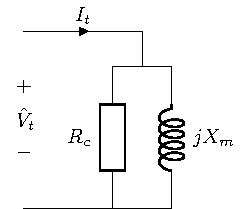
\includegraphics{figTransformersOpenCircuitTest}
\begin{tikzpicture}
%grid
%\draw[gray,thick] (0,-3) grid (15,1);
%\draw[gray,thin,xstep=0.1,ystep=0.1] (0,-3) grid (15,1);
%transformer outer dimensions
\pgfmathsetmacro{\h}{2.5}
\def\ky{-3};
\draw(0,0)  to  [short,i^=$I_t$]  ++(2,0); 
\draw(0,\ky) to ++(2.5,0);
\draw(2,0) to [short,-*]++(0,-0.6);
\draw(1.5,-0.6) to [short] ++(1,0);
\draw(1.5,\ky) to [european resistor,l=$R_c$,*-] ++(0,2.4);
\draw(2.5,\ky) to [inductor,l_=$j X_m$] ++(0,2.4);
%
\draw(0,\ky/2) node{$
\begin{aligned}
&+\\
&\hat{V}_t\\
&-
\end{aligned}
$};
\end{tikzpicture}
\caption{کھلے سرے معائنہ۔}
\label{شکل_ٹرانسفارمر_کھلے_سرے_معائنہ}
\end{figure}

چونکہ برقی طاقت کا ضیاع صرف مزاحمت میں ہی ممکن ہے لہٰذا \عددیء{p_t} صرف  \عددیء{R_c}  میں ہی ضائع ہو گی۔ یوں
\begin{align*}
p_t=\frac{V_t^2}{R_c}
\end{align*}
لکھا جائے گا۔یوں
\begin{align}\label{مساوات_ٹرانسفارمر_کھلے_دور_مزاحمت_حاصل}
R_c&=\frac{V_t^2}{p_t}
\end{align}
حاصل ہوتا ہے۔

اسی طرح چونکہ برقی دباو اور برقی رو کی مقداروں کے تناسب کو برقی رکاوٹ کی مقدار کہتے ہیں لہٰذا
\begin{align*}
\abs{Z_t}=\frac{V_t}{I_t}
\end{align*}
مگر شکل \حوالہ{شکل_ٹرانسفارمر_کھلے_سرے_معائنہ}  سے واضح ہے کہ
\begin{align*}
\frac{1}{Z_t}=\frac{1}{R_c}+\frac{1}{j X_m}
\end{align*}
لہٰذا
\begin{align*}
Z_t&=\frac{j R_c X_m}{R_c+j X_m}\\
\abs{Z_t}&=\frac{R_c X_m}{\sqrt{R_c^2+X_m^2}}
\end{align*}
جس سے حاصل ہوتا ہے
\begin{align}\label{مساوات_ٹرانسفارمر_کھلے_دور_امالہ_حاصل}
X_m=\frac{R_c \abs{Z_t}}{\sqrt{R_c^2-\abs{Z_t}^2}}
\end{align}
مساوات \حوالہ{مساوات_ٹرانسفارمر_کھلے_دور_مزاحمت_حاصل}  سے \عددیء{R_c} اور  مساوات \حوالہ{مساوات_ٹرانسفارمر_کھلے_دور_امالہ_حاصل}  سے  \عددیء{X_m}  کا حساب لگایا جاتا ہے۔

یاد رہے کہ حاصل کردہ \عددیء{R_c} اور \عددیء{X_m} ٹرانسفارمر کے اسی جانب کے لئے درست ہیں جس جانب انہیں حاصل کیا گیا ہو۔اگر ان کی قیمتیں دوسری جانب درکار ہوں تب تبادلہ رکاوٹ کا استعمال کرتے ہوئے اس جانب کی قیمتیں حاصل کی جا سکتی ہیں۔ 

\جزوحصہ{ کسرِ دور معائنہ}
یہ معائنہ بھی پچھلے معائنہ کی طرح ٹرانسفارمر کے کسی بھی طرف کیا جا سکتا ہے مگر حقیقت میں اسے زیادہ برقی دباو کے لچھے پر ہی کرنا زیادہ آسان ہوتا ہے۔ یہ معائنہ جتنے برقی رو کے لئے ٹرانسفارمر بنایا گیا ہو اتنی برقی رو یا اس کے قریب مقدار پر کیا جاتا ہے۔یعنی اس معائنہ میں کوشش ہوتی ہے کہ ٹرانسفارمر کے لچھے میں اتنی برقی رو گزرے جتنی کے لئے یہ بنایا گیا ہو۔ لہٰذا اگر ہم پچھلے معائنہ میں استعمال ہونے والے ٹرانسفارمر کی بات آگے بڑھائیں تو اس کا زیادہ برقی دباو کا لچھا \عددیء{\SI{2.2727}{\ampere}} اور کم برقی دباو کا لچھا \عددیء{\SI{113.63}{\ampere}} کے لئے بنایا گیا ہے۔ لہٰذا اگر یہ معائنہ کم برقی دباو لچھے پر کیا جائے تو اسے \عددیء{\SI{113.63}{\ampere}}  پر  کرنا ہو گا اور اگر زیادہ برقی دباو لچھے پر کیا جائے تو صرف \عددیء{\SI{2.2727}{\ampere}} پر کرنا ہو گا جو کہ زیادہ آسان ہے۔
\begin{figure}
\centering
%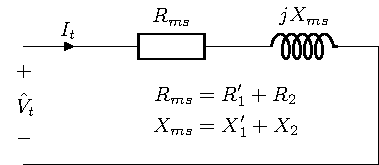
\includegraphics{figTransformersShortCircuitTest}
\begin{tikzpicture}
%grid
%\draw[gray,thick] (0,-4) grid (6,1);
%\draw[gray,thin,xstep=0.1,ystep=0.1] (0,-4) grid (6,1);
%transformer outer dimensions
\pgfmathsetmacro{\h}{2.5}
\def\ky{-2};
\draw(0,0)  to  [short,i=$I_t$]  ++(1.5,0)  to [european resistor,l=$R_{ms}$] ++(2,0) to [inductor,l=$j X_{ms}$]  ++(2.5,0) to [short] ++(0,\ky) to [short] ++(-6,0); 
%
\draw(0,\ky/2) node{$
\begin{aligned}
&+\\
&\hat{V}_t\\
&-
\end{aligned}
$};
%
\draw(2,-0.5) node[below right]{$
\begin{aligned}
R_{ms}&=R_1'+R_2\\
X_{ms}&=X_1'+X_2
\end{aligned}
$};
\end{tikzpicture}
\caption{کسر دور معائنہ۔}
\label{شکل_ٹرانسفارمر_کسر_دور_معائنہ}
\end{figure}

اس معائنہ میں کم برقی دباو لچھے کے دونوں سروں کو آپس میں جوڑا جاتا ہے یعنی انہیں کسرِ دور کر لیا جاتا ہے اور زیادہ برقی دباو لچھے پر اس جانب کی ڈیزائن کردہ برقی دباو کے دو سے بارہ  فی صد کا برقی دباو \عددیء{V_t} لاگو کر کے کسرِ دور برقی رو \عددیء{I_t} اور کسرِ دور برقی طاقت \عددیء{p_t} ناپے جاتے ہیں۔ جس لچھے کے سرے آپس میں کسرِ دور ہوتے ہیں اس میں سے برقی رو گزرتی ہے اور اس کا عکس دوسری جانب بھی موجود ہوتا ہے۔ یہ برقی رو ٹرانسفارمر کے ڈیزائن کردہ برقی رو کے لگ بھگ ہوتا ہے۔ اس معائنہ کا دور شکل \حوالہ{شکل_ٹرانسفارمر_کسر_دور_معائنہ} میں دکھایا گیا ہے۔کھلے سرے معائنے کی طرح اگر کسر دور معائنے میں بھی  شکل \حوالہ{شکل_ٹرانسفارمر_مکمل_ماڈل_ابتدائی_جانب} کے بائیں جانب کو کم برقی دباو والی جانب تصور کریں تو  \عددیء{V_t} کو  \عددیء{V_2} کی جگہ لاگو کرنا ہو گا۔

 چونکہ یہ معائنہ بہت کم برقی دباو پر کیا جاتا ہے لہٰذا اس معائنہ میں ہیجان انگیز برقی رو کو مکمل طور پر نظرانداز کیا جا سکتا ہے۔ شکل سے ہم دیکھتے ہیں کہ چونکہ برقی طاقت صرف مزاحمت میں ہی ضائع ہو سکتی ہے لہٰذا
\begin{align*}
p_t=I_t^2 \left(R_{ms}\right)
\end{align*}
ہو گا جس سے
\begin{align}\label{مساوات_ٹرانسفارمر_کسر_دور_مزاحمت_حاصل}
R_{ms}=\frac{p_t}{I_t^2}
\end{align}
حاصل ہوتا ہے۔

کسرِ دور برقی رو اور برقی دباو سے ہمیں ملتی ہے
\begin{align*}
\abs{Z_t}=\frac{V_t}{I_t}
\end{align*}
مگر شکل سے واضح ہے کہ
\begin{align*}
Z_t&=R_{ms}+j X_{ms}\\
\abs{Z_t}&=\sqrt{R_{ms}^2+X_{ms}^2}
\end{align*}
لہٰذا
\begin{align}\label{مساوات_ٹرانسفارمر_کسر_دور_امالہ_حاصل}
X_{ms}=\sqrt{\abs{Z_t}^2-R_{ms}^2}
\end{align}
مساوات \حوالہ{مساوات_ٹرانسفارمر_کسر_دور_مزاحمت_حاصل} کل مزاحمت دیتا ہے البتہ اس سے \عددی{R_1} یا \عددیء{R_2} حاصل نہیں کیا جا سکتا۔اسی طرح مساوات \حوالہ{مساوات_ٹرانسفارمر_کسر_دور_امالہ_حاصل} سے \عددیء{X_1} اور \عددیء{X_2} علیحدہ نہیں کئے جا سکتے۔کسر دور معائنہ سے اتنی ہی معلومات حاصل کرنا ممکن ہے۔حقیقت میں اتنی معلومات کافی ہوتی ہے۔ اگر ان اجزاء ک علیحدہ علیحدہ قیمتیں درکار ہوں تو ایسی صورت میں تصور کیا جاتا ہے کہ
\begin{align*}
R_1'&=R_2\\
X_1'&=X_2
\end{align*}
ہیں۔

 چونکہ یہ معائنہ عموماً جہاں ٹرانسفارمر موجود ہو وہیں کرنا پڑتا ہے لہٰذا یہ ممکن نہیں ہوتا کہ ٹرانسفارمر کو بالکل اتنا برقی دباو دیا جائے جتنا درکار ہو بلکہ جو برقی دباو موجود ہو اسی سے کام چلانا پڑتا ہے۔ لیکن اس بات کا خیال بہت ضروری ہے کہ جو برقی دباو ٹرانسفارمر کو دیا جا رہا ہو وہ ڈیزائن کردہ برقی دباو کے دو سے بارہ  فی صد ہو۔ مثلاً اگر اسی \عددیء{11000:220\,\textup{V}} ٹرانسفارمر کی بات کی جائے تو اس کے زیادہ برقی دباو لچھے پر \عددیء{\SI{220}{\volt}} اور \عددیء{\SI{1320}{\volt}}  کے درمیان کوئی بھی برقی دباو دیا جا سکتا ہے۔ چونکہ ہمارے ہاں \عددیء{\SI{220}{\volt}}  اور \عددیء{\SI{440}{\volt}}  عام پائے جاتے ہیں لہٰذا ہم \عددیء{\SI{220}{\volt}}  یا \عددیء{\SI{440}{\volt}}  ہی استعمال کریں گے۔

یہاں یہ ایک مرتبہ دوبارہ یاد دھیانی کراتا جاول کہ ٹرانسفارمر کی ایک جانب لچھے کے سرے آپس میں جوڑ کر، یعنی انہیں کسرِ دور کر کے، دوسری جانب لچھے پر کسی بھی صورت میں اس جانب کی پوری برقی دباو لاگو نہیں کرنا۔ ایسا کرنا  شدید  خطرناک اور جان لیوا ثابت ہو سکتا ہے۔

یاد رہے کہ حاصل کردہ \عددیء{R_c} اور \عددیء{X_m} ٹرانسفارمر کے اسی جانب کے لئے درست ہیں جس جانب انہیں حاصل کیا گیا ہو۔اگر ان کی قیمتیں دوسری جانب درکار ہوں تب تبادلہ رکاوٹ کا استعمال کرتے ہوئے اس جانب کی قیمتیں حاصل کی جا سکتی ہیں۔ 
%
\ابتدا{مثال}
ایک \عددیء{25}  کلو وولٹ-ایمپیئر، \عددیء{11000:220} وولٹ اور \عددیء{50} ہرٹز پر چلنے والے ٹرانسفارمر کے کھلے دور اور کسرِ دور معائنہ کئے جاتے ہیں جن کے نتائج یہ ہیں۔
\begin{itemize}
\item
کھلے دور معائنہ کرتے وقت کم برقی دباو کی جانب  \عددیء{\SI{220}{\volt}} لاگو کئے جاتے ہیں۔اسی جانب برقی رو \عددیء{\SI{39.64}{\ampere}} اور طاقت کا ضیاع \عددیء{\SI{600}{\watt}} ناپے جاتے ہیں۔
\item
کسرِ دور معائنہ کرتے وقت زیادہ برقی دباو کی جانب  \عددیء{\SI{440}{\volt}} لاگو کئے جاتے ہیں۔اسی جانب برقی رو \عددیء{\SI{2.27}{\ampere}} اور طاقت کا ضیاع \عددیء{\SI{560}{\watt}} ناپے جاتے ہیں۔
\end{itemize}

کھلے دور حل:
\begin{align*}
\abs{Z_t}&=\frac{220}{39.64}=\SI{5.55}{\ohm}\\
R_c&=\frac{220^2}{600}=\SI{80.67}{\ohm}\\
X_m&=\frac{80.67 \times 5.55}{\sqrt{80.67^2-5.55^2}}=\SI{5.56}{\ohm}
\end{align*}
کسر دور حل:
\begin{align*}
Z_t&=\frac{440}{2.27}=\SI{193.83}{\ohm}\\
R_{ms}&=\frac{560}{2 \times 2.27^2}=\SI{108.68}{\ohm}\\
X_{ms}&=\sqrt{193.83^2-108.68^2}=\SI{160}{\ohm}
\end{align*}

ان نتائج کو کم برقی دباو جانب منتقل کرتے ہوئے 
\begin{align*}
\left(\frac{220}{11000} \right)^2 \times 108.68=\SI{43.47}{\milli \ohm}\\
\left(\frac{220}{11000} \right)^2 \times 160=\SI{64}{\milli \ohm}
\end{align*}
یعنی
\begin{align*}
R_1&=R_2'=\frac{\SI{43.47}{\milli \ohm}}{2}=\SI{21.7}{\milli \ohm}\\
X_1&=X_2'=\frac{\SI{64}{\milli \ohm}}{2}=\SI{32}{\milli \ohm}
\end{align*}
حاصل ہوتا ہے۔ان نتائج سے حاصل کم برقی دباو جانب مساوی دور شکل \حوالہ{شکل_ٹرانسفارمر_کھلے_سرے_کسر_دور_مثال} میں دکھایا گیا ہے۔
\begin{figure}
\centering
%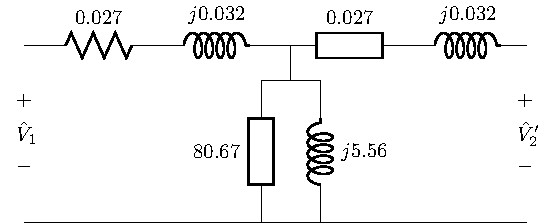
\includegraphics{figTransformersOpenAndShortTestExample}
\begin{tikzpicture}
%grid
%\draw[gray,thick] (0,-4) grid (15,1);
%\draw[gray,thin,xstep=0.1,ystep=0.1] (0,-4) grid (15,1);
%transformer outer dimensions
\pgfmathsetmacro{\h}{2.5}
\def\ky{-3};
\draw(0,0)  to  [short]  ++(0.5,0) to [resistor,l=$0.027$] ++(1.5,0) to [inductor,l=$j 0.032$] ++(2.5,0)coordinate(a){} to
[european resistor,l=$0.027$] ++(2,0) to [inductor,l=$j 0.032 $] ++(2,0); 
\draw(0,\ky) to [short]++(8.5,0);
\draw(a) to [short,*-*] ++(0,-0.6);
\draw(4,-0.6) to [short] ++(1,0);
\draw(4,\ky) to [european resistor,l=$80.67$,*-] ++(0,2.4);
\draw(5,\ky) to [inductor,l_=$j 5.56$,*-] ++(0,2.4);
%
\draw(0,\ky/2) node{$
\begin{aligned}
&+\\
&\hat{V}_1\\
&-
\end{aligned}
$};
%
\draw(8.5,\ky/2) node{$
\begin{aligned}
&+\\
&\hat{V}_2'\\
&-
\end{aligned}
$};
\end{tikzpicture}
\caption{کھلے دور اور کسرِ دور معائنہ سے کم برقی دباو جانب  مساوی دور۔}
\label{شکل_ٹرانسفارمر_کھلے_سرے_کسر_دور_مثال}
\end{figure}
\انتہا{مثال}
%
\حصہ{تین مرحلہ ٹرانسفارمر}
اب تک ہم  \اصطلاح{ایک مرحلہ}\حاشیہب{single phase} ٹرانسفارمر پر غور کرتے رہے ہیں۔حقیقت میں برقی طاقت کی منتقلی میں عموماً \اصطلاح{تین مرحلہ}\فرہنگ{تین مرحلہ}\حاشیہب{three phase}\فرہنگ{three phase} ٹرانسفارمر استعمال ہوتے ہیں۔تین مرحلہ ٹرانسفارمر یکساں تین عدد  ایک مرحلہ  ٹرانسفارمر اکٹھے رکھ کر بنایا جا سکتا ہے۔یوں اگر ایک ٹرانسفارمر خراب ہو جائے تو اس کو ٹھیک ہونے کے لئے ہٹا کر بقایا دو ٹرانسفارمر دوبارہ چالو کئے جا سکتے ہیں۔تین مرحلہ ٹرانسفارمر بنانے کا اس سے بہتر طریقہ شکل \حوالہ{شکل_ٹرانسفارمر_ایک_مرکز_تین-ٹرانسفارمر} میں دکھایا گیا ہے جہاں ایک ہی مقناطیسی قالب پر تینوں ٹرانسفارمر کے لچھے لپٹے گئے ہیں۔اس شکل میں \عددیء{\hat{V}_{i1}} پہلے ٹرانسفارمر کا ابتدائی لچھا جبکہ \عددیء{\hat{V}_{s1}} اس کا ثانوی لچھا ہے۔اس طرح کے تین مرحلہ ٹرانسفارمر سستے، ہلکے اور چھوٹے ہونے کی وجہ سے عام ہو گئے ہیں اور آپ کو روز مرہ زندگی میں یہی نظر آئیں گے۔ان میں برقی ضیاع بھی قدرِ کم ہوتی ہے۔
\begin{figure}
\centering
%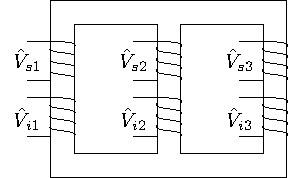
\includegraphics{figTransformersThreePhaseSingleCore}
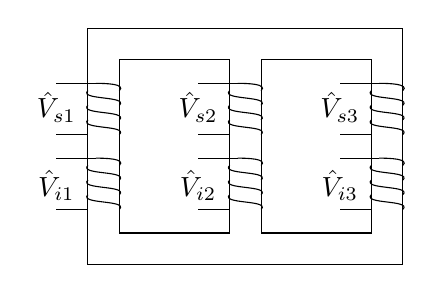
\begin{tikzpicture}
%grid
%\draw[gray,thick] (-1,-1) grid (5,3);
%\draw[gray,thin,xstep=0.1,ystep=0.1] (-1,-1) grid (5,3);
%transformer outer dimensions
\pgfmathsetmacro{\h}{3}
\pgfmathsetmacro{\w}{4}
\pgfmathsetmacro{\t}{0.4}
\pgfmathsetmacro{\g}{0.3}   %gap between coil and edge of window
\pgfmathsetmacro{\nL}{4}       %number of left hand turns
\pgfmathsetmacro{\nR}{3}      %number of right hand turns
%window size
\pgfmathsetmacro{\winH}{\h-2*\t}
\pgfmathsetmacro{\winW}{0.5*(\w-3*\t)}
%coil step
\pgfmathsetmacro{\stepHL}{0.5*(\h-2*\t-3*\g)/(\nL-0.5)}
\pgfmathsetmacro{\stepHR}{0.5*(\h-2*\t-3*\g)/(\nR-0.5)}

%transformer
\draw(0,0) rectangle (\w,\h);
\draw(\t,\t) rectangle ++(\winW,\winH);
\draw(2*\t+\winW,\t) rectangle ++(\winW,\winH);
%----------------------
%========================
%left leg TOP coil. top to bottom
\def\leftEdge{0};
\def\coilTop{\h-\t-\g};
%
\draw(\leftEdge+\t/4,\coilTop) to [out=0,in=45] (\leftEdge+\t,{\coilTop-\stepHL/2}); %top half section
%coil itself
\pgfmathsetmacro{\nLend}{\nL-2}
\foreach \y in { 0, ..., \nLend }{
\draw (\leftEdge,{\coilTop-\stepHL/2-\y*\stepHL}) to [out=-135,in=45] (\leftEdge+\t,{\coilTop-\stepHL/2-\y*\stepHL-\stepHL});
} 
%left hand terminals
\draw (\leftEdge+\t/4,\coilTop)--++(-1.25*\t,0) node(TA.A1){};
\draw (\leftEdge,\coilTop-\nL*\stepHL+0.5*\stepHL)--++(-1*\t,0)node(TA.A2){};
%--------------------
%left leg BOTTOM coil. top to bottom
\def\leftEdge{0};
\def\coilTop{\h-\t-2*\g-\nL*\stepHL+0.5*\stepHL};
%
\draw(\leftEdge+\t/4,\coilTop) to [out=0,in=45] (\leftEdge+\t,{\coilTop-\stepHL/2}); %top half section
%coil itself
\pgfmathsetmacro{\nLend}{\nL-2}
\foreach \y in { 0, ..., \nLend }{
\draw (\leftEdge,{\coilTop-\stepHL/2-\y*\stepHL}) to [out=-135,in=45] (\leftEdge+\t,{\coilTop-\stepHL/2-\y*\stepHL-\stepHL});
} 
%left hand terminals
\draw (\leftEdge+\t/4,\coilTop)--++(-1.25*\t,0) node(TA.B1){};
\draw (\leftEdge,\coilTop-\nL*\stepHL+0.5*\stepHL)--++(-1*\t,0)node(TA.B2){};
%==========================
%============================
%middle leg TOP coil. top to bottom
\def\leftEdge{\t+\winW};
\def\coilTop{\h-\t-\g};
%
\draw(\leftEdge+\t/4,\coilTop) to [out=0,in=45] (\leftEdge+\t,{\coilTop-\stepHL/2}); %top half section
%coil itself
\pgfmathsetmacro{\nLend}{\nL-2}
\foreach \y in { 0, ..., \nLend }{
\draw (\leftEdge,{\coilTop-\stepHL/2-\y*\stepHL}) to [out=-135,in=45] (\leftEdge+\t,{\coilTop-\stepHL/2-\y*\stepHL-\stepHL});
} 
%left hand terminals
\draw (\leftEdge+\t/4,\coilTop)--++(-1.25*\t,0) node(TB.A1){};
\draw (\leftEdge,\coilTop-\nL*\stepHL+0.5*\stepHL)--++(-1*\t,0)node(TB.A2){};
%--------------------
%middle  leg BOTTOM coil. top to bottom
\def\leftEdge{\t+\winW};
\def\coilTop{\h-\t-2*\g-\nL*\stepHL+0.5*\stepHL};
%
\draw(\leftEdge+\t/4,\coilTop) to [out=0,in=45] (\leftEdge+\t,{\coilTop-\stepHL/2}); %top half section
%coil itself
\pgfmathsetmacro{\nLend}{\nL-2}
\foreach \y in { 0, ..., \nLend }{
\draw (\leftEdge,{\coilTop-\stepHL/2-\y*\stepHL}) to [out=-135,in=45] (\leftEdge+\t,{\coilTop-\stepHL/2-\y*\stepHL-\stepHL});
} 
%left hand terminals
\draw (\leftEdge+\t/4,\coilTop)--++(-1.25*\t,0) node(TB.B1){};
\draw (\leftEdge,\coilTop-\nL*\stepHL+0.5*\stepHL)--++(-1*\t,0)node(TB.B2){};
%===========================
%============================
%right leg TOP coil. top to bottom
%========================
\def\leftEdge{\w-\t};
\def\coilTop{\h-\t-\g};
%
\draw(\leftEdge+\t/4,\coilTop) to [out=0,in=45] (\leftEdge+\t,{\coilTop-\stepHL/2}); %top half section
%coil itself
\pgfmathsetmacro{\nLend}{\nL-2}
\foreach \y in { 0, ..., \nLend }{
\draw (\leftEdge,{\coilTop-\stepHL/2-\y*\stepHL}) to [out=-135,in=45] (\leftEdge+\t,{\coilTop-\stepHL/2-\y*\stepHL-\stepHL});
} 
%left hand terminals
\draw (\leftEdge+\t/4,\coilTop)--++(-1.25*\t,0) node(TC.A1){};
\draw (\leftEdge,\coilTop-\nL*\stepHL+0.5*\stepHL)--++(-1*\t,0)node(TC.A2){};
%--------------------
%right leg BOTTOM coil. top to bottom
\def\leftEdge{\w-\t};
\def\coilTop{\h-\t-2*\g-\nL*\stepHL+0.5*\stepHL};
%
\draw(\leftEdge+\t/4,\coilTop) to [out=0,in=45] (\leftEdge+\t,{\coilTop-\stepHL/2}); %top half section
%coil itself
\pgfmathsetmacro{\nLend}{\nL-2}
\foreach \y in { 0, ..., \nLend }{
\draw (\leftEdge,{\coilTop-\stepHL/2-\y*\stepHL}) to [out=-135,in=45] (\leftEdge+\t,{\coilTop-\stepHL/2-\y*\stepHL-\stepHL});
} 
%left hand terminals
\draw (\leftEdge+\t/4,\coilTop)--++(-1.25*\t,0) node(TC.B1){};
\draw (\leftEdge,\coilTop-\nL*\stepHL+0.5*\stepHL)--++(-1*\t,0)node(TC.B2){};
%==========================
%===========================
%text
\draw (-0.4,1) node{$\hat{V}_{i1}$};
\draw (-0.4,2) node{$\hat{V}_{s1}$};
\draw (1.4,1) node{$\hat{V}_{i2}$};
\draw (1.4,2) node{$\hat{V}_{s2}$};
\draw (3.2,1) node{$\hat{V}_{i3}$};
\draw (3.2,2) node{$\hat{V}_{s3}$};
\end{tikzpicture}
\caption{ایک ہی قالب پر تین ٹرانسفارمر۔}
\label{شکل_ٹرانسفارمر_ایک_مرکز_تین-ٹرانسفارمر}
\end{figure}

شکل \حوالہ{شکل_ٹرانسفارمر_ستارہ_تکونی_جوڑ}-الف میں تین ٹرانسفارمر دکھائے گئے ہیں۔ان تین ٹرانسفارمر کے ابتدائی لچھے آپس میں دو طریقوں سے جوڑے جا سکتے ہیں۔ایک کو \اصطلاح{ستارہ نما} جوڑ\فرہنگ{ستارہ نما جوڑ}\فرہنگ{جوڑ!ستارہ نما}\حاشیہب{star connected}\فرہنگ{star connected} \عددیء{Y}  اور دوسرے کو \اصطلاح{تکونی} جوڑ\فرہنگ{تکونی جوڑ}\فرہنگ{جوڑ!تکونی}\حاشیہب{delta connected}\فرہنگ{delta connected}  \عددیء{\Delta}   کہتے ہیں۔اسی طرح ان تینوں ٹرانسفارمروں کے ثانوی  لچھے انہیں دو طریقوں سے جوڑے جا سکتے ہیں۔یوں انہیں جوڑنے کے چار ممکنہ طریقے ہیں یعنی
\begin{itemize}
\item
ستارہ:تکونی  \quad \عددیء{Y:\Delta}
\item
ستارہ:ستارہ \quad  \عددیء{Y:Y}
\item
تکونی:تکونی \quad  \عددیء{\Delta:\Delta}
\item
تکونی:ستارہ  \quad  \عددیء{\Delta:Y}
\end{itemize}

شکل \حوالہ{شکل_ٹرانسفارمر_ستارہ_تکونی_جوڑ}-الف میں ان تین ٹرانسفارمروں کے ابتدائی لچھوں کو ستارہ نما جوڑا گیا ہے جبکہ ان کی ثانوی لچھوں کو تکونی جوڑا گیا ہے۔شکل-ب میں تینوں ٹرانسفارمر کی ابتدائی لچھوں کو  ستارہ نما  دکھایا گیا ہے۔اسی طرح ثانوی لچھوں کو تکونی  دکھایا گیا ہے۔انہی شکلوں کی وجہ سے ان کو ستارہ نما جوڑ اور تکونی جوڑ کہتے ہیں۔

ایسی شکل بناتے وقت تینوں ٹرانسفارمروں کے ابتدائی لچھے کو جس زاویہ پر بنایا جاتا ہے اس کے ثانوی لچھے کو بھی اسی زاویہ پر بنایا جاتا ہے۔یوں شکل کے حصہ الف میں سب سے اوپر ٹرانسفارمر جس کے ابتدائی جانب کے  سرے \عددیء{an} اور ثانوی جانب  کے سرے \عددیء{a'n'} ہیں کو حصہ با میں صفر زاویہ پر بنایا گیا ہے۔تین  مرحلہ ٹرانسفارمروں کو اس طرح کی علامتوں سے ظاہر کیا جاتا ہے اور ان میں قالب نہیں دکھایا جاتا۔

ٹرانسفارمر کے جوڑ بیان کرتے وقت بائیں جانب کے جوڑ کو پہلے اور دائیں جانب کی جوڑ کو بعد میں پکارتے ہیں۔یوں شکل میں ٹرانسفارمر کو ستارہ-تکونی جڑا ٹرانسفارمر کہیں گے۔اسی طرح ابتدائی جانب کو بائیں اور ثانوی جانب کو دائیں ہاتھ بنایا جاتا ہے۔یوں اس شکل میں ابتدائی جانب ستارہ نما ہے جبکہ ثانوی جانب تکونی ہے۔
\begin{figure}
\centering
%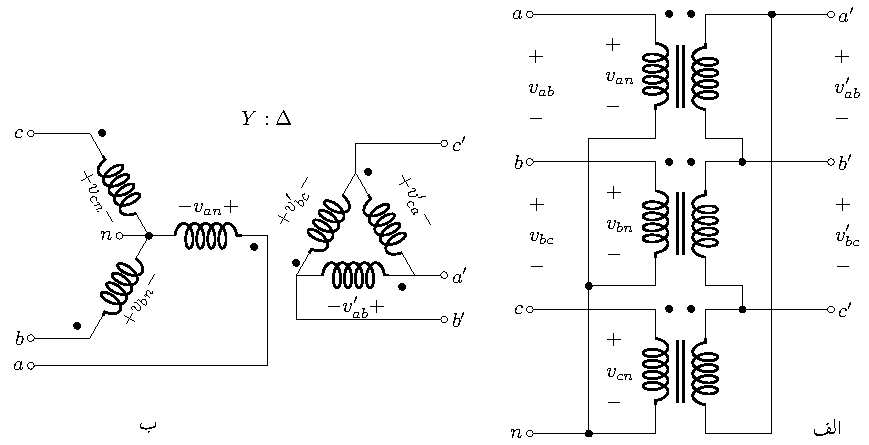
\includegraphics[width=\linewidth]{figTransformersStarDeltaConnections}
\begin{tikzpicture}[scale=0.75]
%grid
%\draw[gray,thick] (-3,-3) grid (12,5);
%\draw[gray,thin,xstep=0.1,ystep=0.1] (-3,-3) grid (12,5);
%transformer outer dimensions
\pgfmathsetmacro{\l}{1.5}
\pgfmathsetmacro{\s}{0.5}
\pgfmathsetmacro{\arm}{2}
\pgfmathsetmacro{\shiftX}{9cm}
\pgfmathsetmacro{\shiftY}{1.25 cm}
\pgfmathsetmacro{\gap}{3.5 cm}
\pgfmathsetmacro{\startDelX}{-\arm/2}
\pgfmathsetmacro{\startDelY}{-\arm/3}
\draw node at (11.5,-2) {الف};
\draw node at (0,-2) {ب};
%
\begin{scope}[xshift=\shiftX]
\draw (0,0) node  [transformer core](T1){}; 
\draw (0,2.5) node  [transformer core](T2){}; 
\draw (0,5) node  [transformer core](T3){}; 
\draw(T1.base) node {$\bullet \hspace{2mm} \bullet$};
\draw(T2.base) node {$\bullet \hspace{2mm} \bullet$};
\draw(T3.base) node {$\bullet \hspace{2mm} \bullet$};
%
\draw(T1.A1) to [short,-o] ++(-\l,0) node[left](c) {$c$};
\draw(T2.A1) to [short,-o] ++(-\l,0) node[left](b) {$b$};
\draw(T3.A1) to [short,-o] ++(-\l,0) node[left] (a){$a$};
%
\draw(T1.A2) to [short,-*] ++(-\s,0) coordinate (k1){};
\draw(T2.A2) to [short,-*] ++(-\s,0)coordinate (k2){};
\draw(T3.A2) to [short] ++(-\s,0)coordinate (k3){};
%
\draw(k3) to [short] (k2) to [short] (k1) to [short,-o] ++(-\l+\s,0)node[left](n){$n$};
%text
\node[right] at ($(a) ! 0.5 ! (b)$) {$
\begin{aligned}
&+\\
&v_{ab}\\
&-
\end{aligned}
$};
%
\node[right] at ($(b) ! 0.5 ! (c)$) {$
\begin{aligned}
&+\\
&v_{bc}\\
&-
\end{aligned}
$};
%
\node at ($(T1.A1) ! 0.5 ! (T1.A2)$){$
\begin{aligned}
&+\\
&v_{cn}\\
&-
\end{aligned}
$};
%
\node at ($(T2.A1) ! 0.5 ! (T2.A2)$){$
\begin{aligned}
&+\\
&v_{bn}\\
&-
\end{aligned}
$};
%
\node at ($(T3.A1) ! 0.5 ! (T3.A2)$){$
\begin{aligned}
&+\\
&v_{an}\\
&-
\end{aligned}
$};
%right hand side
\draw(T1.B1) to [short,-o] ++(\l,0)  node[right](c'){$c'$};
\draw(T2.B1) to [short,-o] ++(\l,0)node[right](b'){$b'$};
\draw(T3.B1) to [short,-o] ++(\l,0) node [right](a'){$a'$};
%;
\draw(T1.B2) to [short] ++(\s,0) to [short,-*] ++(0,7.1);
\draw(T2.B2) to [short,-*] (T1.B1);
\draw(T3.B2) to [short,-*] (T2.B1);
%text
\draw node at ($(a') ! 0.5 ! (b')$){$
\begin{aligned}
&+\\
&v_{ab}'\\
&-
\end{aligned}
$};
%
\draw node at ($(b') ! 0.5 ! (c')$){$
\begin{aligned}
&+\\
&v_{bc}'\\
&-
\end{aligned}
$};
\end{scope}
%=====================
\begin{scope}[yshift=\shiftY]
%star
\draw (0,0) to [inductor,l={$- v_{an} +$}] ++(0:\arm)node [below left] {$\bullet$} to [short] ++(0,-2.2) to [short,-o]++(-4,0) node[left] {$a$};
\draw (0,0) to [inductor,l={$+ v_{cn} -$}] ++(120:\arm) node [right]{$\bullet$} to [short,-o] ++(-1,0) node [left] {$c$};
\draw (0,0) to [inductor,l={$+ v_{bn} -$}] ++(-120:\arm) node [above left] {$\bullet$} to [short,-o] ++(-1,0)node [left]{$b$};
\draw (0,0) to [short,*-o] ++(-0.5,0) node [left]{$n$};
\draw(2,2) node {$Y:\Delta$};
%delta
\begin{scope}[xshift=\gap]
\draw (\startDelX,\startDelY) to [inductor,l_={$- v_{ab}'+$}] ++(0:\arm)coordinate(delA){} to [inductor] ++(120:\arm)coordinate(delB){}  to [inductor] ++(-120:\arm);
\path  (30:0.6*\arm)  node[rotate=-60] {$+ v_{ca}' -$}; 
\path  (150:0.6*\arm)  node[rotate=60] {$+ v_{bc}' -$}; 
\draw (delA) to [short,-o] ++(\s,0) node[right]{$a'$};
\draw (delB) to [short] ++(0,0.5) to [short,-o] ++(1.5,0) node[right]{$c'$};
\draw (\startDelX,\startDelY) to [short] ++(0,-0.75) to [short,-o] ++(\l+1,0)node[right]{$b'$};
\draw[below left]  node at (delA){$\bullet$};
\draw[right]  node at (delB){$\bullet$};
\draw[above]  node at (\startDelX,\startDelY){$\bullet$};
\end{scope}
\end{scope}
\end{tikzpicture}
\caption{تین مرحلہ ستارہ-تکونی ٹرانسفارمر}
\label{شکل_ٹرانسفارمر_ستارہ_تکونی_جوڑ}
\end{figure}


	ستارہ نما جڑی جانب سے چار برقی تاریں نکلتی ہیں۔اس جانب لچھوں کے مشترکہ سرا \عددیء{n} کو عموماً ٹرانسفارمر کے نزدیک زمین میں گہرائی تک دھنسا دیا جاتا ہے۔اس تار کو \اصطلاح{زمینی تار}\فرہنگ{زمینی تار}\حاشیہب{ground}\فرہنگ{ground wire}  یا صرف \اصطلاح{زمین}\فرہنگ{زمین}\حاشیہب{ground, earth,neutral}\فرہنگ{earth}  کہتے ہیں۔عام فہم میں اسے \اصطلاح{ٹھنڈی تار}\فرہنگ{ٹھنڈی تار}\حاشیہب{neutral} کہتے ہیں۔باقی تین یعنی \عددیء{a,b,c}  \اصطلاح{گرم تار}\فرہنگ{گرم تار}\حاشیہب{live wires} کہلاتے ہیں۔

ٹرانسفارمر کی لچھے پر برقی دباو کو \اصطلاح{یک مرحلہ برقی دباو}\فرہنگ{یک مرحلہ برقی دباو} \عددیء{\hat{V}_{\textup{یکمرحلہ}}}\حاشیہب{phase voltage}\فرہنگ{phase voltage} کہتے ہیں اور لچھے میں برقی رو کو \اصطلاح{یک مرحلہ برقی رو}\فرہنگ{یک مرحلہ برقی رو} \عددیء{\hat{I}_{\textup{یکمرحلہ}}}\حاشیہب{phase current}\فرہنگ{phase current}  کہتے ہیں۔ جبکہ ٹرانسفارمر سے باہر نکلتی کسی دو گرم تاروں کے مابین برقی دباو کو \اصطلاح{تار کی برقی دباو}\فرہنگ{تار کی برقی دباو} \عددیء{\hat{V}_{\textup{تار}}}\حاشیہب{line to line voltage}\فرہنگ{line voltage} کہتے ہیں اور کسی بھی گرم تار میں برقی رو کو \اصطلاح{تار کی برقی رو}\فرہنگ{تار کی برقی رو} \عددیء{\hat{I}_{\textup{تار}}}\حاشیہب{line current}\فرہنگ{line current}  کہتے ہیں۔ زمینی تار میں برقی رو کو \اصطلاح{زمینی برقی رو}\فرہنگ{زمینی برقی رو}  \عددیء{\hat{I}_{\textup{زمینی}}}\حاشیہب{ground current}\فرہنگ{ground current} کہتے ہیں۔

ستارہ نما \عددیء{Y} جانب \اصطلاح{یک مرحلہ} مقداروں اور \اصطلاح{تار} کی مقداروں  کا آپس میں یوں رشتہ ہے
\begin{gather}
\begin{aligned}\label{مساوات_ستارہ_ٹرانسفارمر_تار_اور_دور_رشتے}
V_{\textup{تار}}&=\sqrt{3} V_{\textup{یکمرحلہ}}\\
I_{\textup{تار}}&=I_{\textup{یکمرحلہ}}
\end{aligned}
\end{gather}
جبکہ تکونی \عددیء{\Delta} جانب یک مرحلہ اور تار کی مقداروں کا آپس میں یوں رشتہ ہے
\begin{gather}
\begin{aligned}\label{مساوات_تکونی_ٹرانسفارمر_تار_اور_دور_رشتے}
V_{\textup{تار}}&= V_{\textup{یکمرحلہ}}\\
I_{\textup{تار}}&=\sqrt{3} I_{\textup{یکمرحلہ}}
\end{aligned}
\end{gather}
یہ مرحلی سمتیہ کے رشتے نہیں بلکہ ان کی غیر سمتی قیمتوں کے رشتے ہیں۔ان دو مساواتوں سے حاصل ہوتا ہے
\begin{align}
V_{\textup{تار}} I_{\textup{تار}}=\sqrt{3} V_{\textup{یکمرحلہ}} I_{\textup{یکمرحلہ}}
\end{align}
چونکہ ایک مرحلہ ٹرانسفارمر کی وولٹ-ایمپیئر \عددیء{V_{\textup{یکمرحلہ}} I_{\textup{یکمرحلہ}}} ہیں اور ایسے تین ٹرانسفارمر مل کر ایک تین مرحلہ ٹرانسفارمر بناتے ہیں لہٰذا تین  مرحلہ ٹرانسفارمر کی وولٹ-ایمپیئر اس کے تین گنا ہوں گے یعنی
\begin{align}
\textup{وولٹ-ایمپیئر}= 
3 V_{\textup{یکمرحلہ}} I_{\textup{یکمرحلہ}}= 
3 \times \frac{V_{\textup{تار}} I_{\textup{تار}}}{\sqrt{3}}=
\sqrt{3} V_{\textup{تار}} I_{\textup{تار}}
\end{align}
یہ مساوات \اصطلاح{تین مرحلہ} ادوار  میں عام استعمال ہوتی ہے۔

	ٹرانسفارمر کسی طرح بھی جوڑے جائیں وہ اپنی بنیادی کارکردگی تبدیل نہیں کرتے لہٰذا انہیں ستارہ نما یا تکونی جوڑنے کے بعد بھی ان میں ہر ایک ٹرانسفارمر انفرادی طور پر صفحہ \حوالہصفحہ{مساوات_ٹرانسفارمر_تبادلہ_دباو_رو} پر دئے مساوات \حوالہ{مساوات_ٹرانسفارمر_تبادلہ_دباو_رو}  اور صفحہ \حوالہصفحہ{مساوات_ٹرانسفارمر_متبادل_رکاوٹ_تعریف} پر دئے مساوات \حوالہ{مساوات_ٹرانسفارمر_متبادل_رکاوٹ_تعریف}  پر پورے اترے گا۔انہیں استعمال کر کے شکل \حوالہ{شکل_ٹرانسفارمر_تین_دور_ٹرانسفارمر_کے_مختلف_جوڑ}  میں دیئے گئے ٹرانسفارمروں کے ابتدائی اور ثانوی جانب کی یک مرحلہ اور تار کی مقداروں کے رشتے حاصل کئے جا سکتے ہیں۔اس شکل میں \عددیء{a=N_1/N_2} ہے جہاں  \عددیء{N_1:N_2} ان میں ایک مرحلہ ٹرانسفارمر کے چکر کی نسبت ہے۔تین مرحلہ ٹرانسفارمر پر لگی تختی پر دونوں جانب تار کی برقی دباو کی نسبت لکھی جاتی ہے۔
\begin{figure}
\centering
%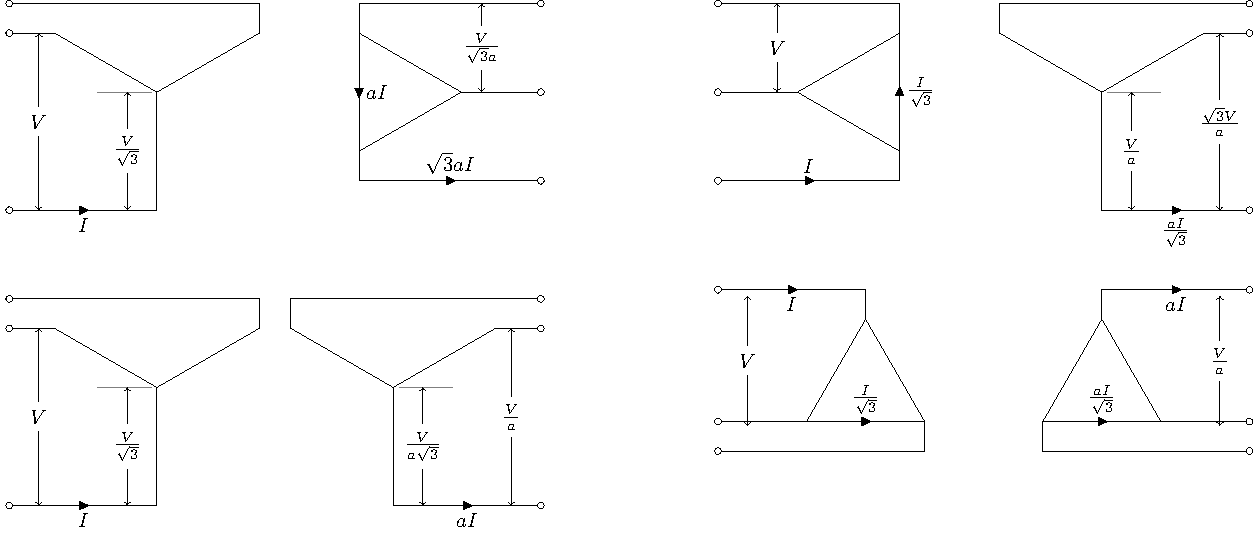
\includegraphics[width=\linewidth]{figTransformersAllPossibleConnections}
\begin{tikzpicture}[scale=0.6]
%grid
%\draw[gray,thick] (-3,-3) grid (18,5);
%\draw[gray,thin,xstep=0.1,ystep=0.1] (-3,-3) grid (18,5);
%transformer outer dimensions
\pgfmathsetmacro{\shiftX}{12 cm}
\pgfmathsetmacro{\shiftY}{5 cm}

\pgfmathsetmacro{\arm}{2}
\pgfmathsetmacro{\con}{2.5}
\pgfmathsetmacro{\conStarS}{\con-\arm*cos(30)}                  %one arm of star is at ninty degree
\pgfmathsetmacro{\conStarL}{\con+\arm*cos(30)}
\pgfmathsetmacro{\h}{sqrt(3)/2*\arm}
\pgfmathsetmacro{\conDeltaS}{\con-\arm/sqrt(3)}                      %one arm of delta is at 90 degree as h=sqrt{3}/2*\arm
\pgfmathsetmacro{\conDeltaL}{\con+\arm/sqrt(12)}
\pgfmathsetmacro{\conDeltaZeroS}{\con-\arm*cos(60)}    %one arm of delta is at 0 degree as h=sqrt{3}/2*\arm
\pgfmathsetmacro{\conDeltaZeroM}{\con}
\pgfmathsetmacro{\conDeltaZeroL}{\con+\arm*cos(60)}


\pgfmathsetmacro{\gap}{4 cm}        %gap between star and delta centres
\pgfmathsetmacro{\startNintyX}{-\h/3}    %start of delta if one arm is at 90 degrees
\pgfmathsetmacro{\startNintyY}{-\arm/2}
\pgfmathsetmacro{\startZeroX}{-\arm/2}   %start of delta if one arm is at 0 degrees
\pgfmathsetmacro{\startZeroY}{-\h/3} 

%===================
%STAR-DELTA
\begin{scope}[yshift=\shiftY]
%star at 90 degrees
\draw (0,0) to [short] ++(-90:\arm)coordinate (starA){} to [short,-o,i<={$I$}] ++(180:\con)coordinate (starAend){};
\draw (0,0) to [short] ++(30:\arm)coordinate (starB){} to [short] ++(0,0.5) to [short,-o]++(180:\conStarL)coordinate (starBend){};
\draw (0,0) to [short] ++(150:\arm)coordinate (starC){} to  [short,-o]++(180:\conStarS)coordinate (starCend){};
%text
\draw[<->](-2,1)--(-2,-2) node[fill=white,pos=0.5]{$V$};
\draw[gray] (-0.1,0)--(-1,0);
\draw[<->](-0.6,0)--(-0.6,-2) node[fill=white,pos=0.5]{$\frac{V}{\sqrt{3}}$};
%=================
%delta at 90 degrees
\begin{scope}[xshift=\gap]
\draw (\startNintyX,\startNintyY)coordinate (deltaNintyA){} to [short] ++(30:\arm)coordinate (deltaNintyB){} to [short] ++(150:\arm)coordinate (deltaNintyC){} to [short,i={$aI$}]++(-90:\arm);
\draw (deltaNintyA) to [short]++(0,-0.5) to [short,-o,i={$\sqrt{3} a I$}] ++(\conDeltaL,0);
\draw (deltaNintyB) to [short,-o] ++(\conDeltaS,0);
\draw (deltaNintyC) to [short]++(0,0.5) to [short,-o] ++(\conDeltaL,0);
\draw[<->](1.6,0)--(1.6,1.5) node [fill=white,pos=0.5]{$\frac{V}{\sqrt{3} a}$};
\end{scope}
%=================================
%=================================
%DELTA-STAR
\begin{scope}[xshift=\shiftX+\gap, xscale=-1, yscale=1]
%star at 90 degrees
\draw (0,0) to [short] ++(-90:\arm)coordinate (starA){} to [short,-o,i<={$\frac{aI}{\sqrt{3}}$}] ++(180:\con)coordinate (starAend){};
\draw (0,0) to [short] ++(30:\arm)coordinate (starB){} to [short] ++(0,0.5) to [short,-o]++(180:\conStarL)coordinate (starBend){};
\draw (0,0) to [short] ++(150:\arm)coordinate (starC){} to  [short,-o]++(180:\conStarS)coordinate (starCend){};
%text
\draw[<->](-2,1)--(-2,-2) node[fill=white,pos=0.5]{$\frac{\sqrt{3}V}{a}$};
\draw[gray] (-0.1,0)--(-1,0);
\draw[<->](-0.5,0)--(-0.5,-2) node[fill=white,pos=0.5]{$\frac{V}{a}$};
%=================
%delta at 90 degrees
\begin{scope}[xshift=\gap]
\draw (\startNintyX,\startNintyY)coordinate (deltaNintyA){} to [short] ++(30:\arm)coordinate (deltaNintyB){} to [short] ++(150:\arm)coordinate (deltaNintyC){} to [short,i<={$\frac{I}{\sqrt{3}}$}]++(-90:\arm);
\draw (deltaNintyA) to [short]++(0,-0.5) to [short,-o,i={$I$}] ++(\conDeltaL,0);
\draw (deltaNintyB) to [short,-o] ++(\conDeltaS,0);
\draw (deltaNintyC) to [short]++(0,0.5) to [short,-o] ++(\conDeltaL,0);
\draw[<->](1.5,0)--(1.5,1.5) node [fill=white,pos=0.5]{$V$};
\end{scope}
\end{scope}
%----======----
\end{scope}
%====================
%===================
%===================
%LOWER TWO FIGURES
%STAR-STAR
%star at 90 degrees
\draw (0,0) to [short] ++(-90:\arm)coordinate (starA){} to [short,-o,i<={$I$}] ++(180:\con)coordinate (starAend){};
\draw (0,0) to [short] ++(30:\arm)coordinate (starB){} to [short] ++(0,0.5) to [short,-o]++(180:\conStarL)coordinate (starBend){};
\draw (0,0) to [short] ++(150:\arm)coordinate (starC){} to  [short,-o]++(180:\conStarS)coordinate (starCend){};
%text
\draw[<->](-2,1)--(-2,-2) node[fill=white,pos=0.5]{$V$};
\draw[gray] (-0.1,0)--(-1,0);
\draw[<->](-0.6,0)--(-0.6,-2) node[fill=white,pos=0.5]{$\frac{V}{\sqrt{3}}$};
%=================
\begin{scope}[xshift=\gap,xscale=-1,yscale=1]
%star at 90 degrees
\draw (0,0) to [short] ++(-90:\arm)coordinate (starA){} to [short,-o,i<={$a I$}] ++(180:\con)coordinate (starAend){};
\draw (0,0) to [short] ++(30:\arm)coordinate (starB){} to [short] ++(0,0.5) to [short,-o]++(180:\conStarL)coordinate (starBend){};
\draw (0,0) to [short] ++(150:\arm)coordinate (starC){} to  [short,-o]++(180:\conStarS)coordinate (starCend){};
%text
\draw[<->](-2,1)--(-2,-2) node[fill=white,pos=0.5]{$\frac{V}{a}$};
\draw[gray] (-0.1,0)--(-1,0);
\draw[<->](-0.8,0)--(-0.8,-2) node[fill=white,pos=0.5]{$\frac{V}{a\sqrt{3}}$};
\end{scope}
%
 % DELTA-DELTA
%delta
\begin{scope}[xshift=\shiftX]
\draw(\startZeroX,\startZeroY)coordinate(deltA){} to [short,i={$\frac{I}{\sqrt{3}} $}] ++(0:\arm)coordinate(deltB){} to [short]++(120:\arm)coordinate(deltC){} to [short] ++(-120:\arm);
\draw[short] (deltA) to [short,-o]++(180:\conDeltaZeroS);
\draw[short] (deltB) to [short] ++(0,-0.5) to [short,-o]++(180:\conDeltaZeroL);
\draw[short] (deltC) to [short] ++(0,0.5) to [short,-o,i<={$I$}]++(180:\conDeltaZeroM);
\draw[<->] (-2,-0.65) --++(0,2.2)node[fill=white,pos=0.5]{$V$};
%delta
\begin{scope}[xshift=\gap,xscale=-1,yscale=1]
\draw(\startZeroX,\startZeroY)coordinate(deltA){} to [short,i={$\frac{a I}{\sqrt{3}} $}] ++(0:\arm)coordinate(deltB){} to [short]++(120:\arm)coordinate(deltC){} to [short] ++(-120:\arm);
\draw[short] (deltA) to [short,-o]++(180:\conDeltaZeroS);
\draw[short] (deltB) to [short] ++(0,-0.5) to [short,-o]++(180:\conDeltaZeroL);
\draw[short] (deltC) to [short] ++(0,0.5) to [short,-o,i<={$a I$}]++(180:\conDeltaZeroM);
\draw[<->] (-2,-0.65) --++(0,2.2)node[fill=white,pos=0.5]{$\tfrac{V}{a}$};
\end{scope}
\end{scope}
\end{tikzpicture}
\caption{ابتدائی اور ثانوی جانب تار اور یک مرحلہ مقداروں کے رشتے۔}
\label{شکل_ٹرانسفارمر_تین_دور_ٹرانسفارمر_کے_مختلف_جوڑ}
\end{figure}


جیسے شکل \حوالہ{شکل_ٹرانسفارمر_تین_دور_ٹرانسفارمر_کے_مختلف_جوڑ} میں دکھایا گیا ہے ستارہ-تکونی ٹرانسفارمر کی تار پر برقی دباو کی نسبت
\begin{align}
\frac{V_\textup{{ابتدائی}}}{V_\textup{{ثانوی}}}=\sqrt{3} a =\sqrt{3} \left(\frac{N_1}{N_2} \right)
\end{align}
جبکہ ستارہ-ستارہ کا
\begin{align}
\frac{V_\textup{{ابتدائی}}}{V_\textup{{ثانوی}}}=a =\left(\frac{N_1}{N_2} \right)
\end{align}
تکونی-ستارہ کا
\begin{align}
\frac{V_\textup{{ابتدائی}}}{V_\textup{{ثانوی}}}=\frac{a}{\sqrt{3}}=\frac{1}{\sqrt{3}} \left(\frac{N_1}{N_2} \right)
\end{align}
اور تکونی-تکونی کا
\begin{align}
\frac{V_\textup{{ابتدائی}}}{V_\textup{{ثانوی}}}=a =\left(\frac{N_1}{N_2} \right)
\end{align}
ہے۔
%
\ابتدا{مثال}
یک مرحلہ  تین یکساں ٹرانسفارمروں کو ستارہ-تکونی \عددیء{Y:\Delta}  جوڑ کر تین مرحلہ ٹرانسفارمر بنایا گیا ہے۔ایک مرحلہ ٹرانسفارمر کی برقی \اصطلاح{سکت}\فرہنگ{سکت}\حاشیہب{rating}\فرہنگ{rating} درج ذیل ہے:
\begin{align*}
\SI{50}{\kilo \volt \ampere} , \quad 6350:440\,\textup{V}, \quad \SI{50}{\hertz}
\end{align*}
ستارہ-تکونی ٹرانسفارمر کی ابتدائی جانب \عددیء{11000}  وولٹ کی تین مرحلہ تار کی برقی دباو لاگو کیا گیا۔اس تین مرحلہ ٹرانسفارمر کی ثانوی جانب تار کا برقی دباو معلوم کریں۔

حل: حل کرتے وقت ہم ایک  عدد  یک مرحلہ ٹرانسفارمر پر نظر رکھیں گے۔ ابتدائی جانب اگر یک مرحلہ ٹرانسفارمر پر غور کیا جائے تو
\begin{align*}
\frac{N_1}{N_2}=\frac{V_1}{V_2}=\frac{6350}{440}
\end{align*}
اور اس پر لاگو برقی دباو مساوات \حوالہ{مساوات_ستارہ_ٹرانسفارمر_تار_اور_دور_رشتے}  کی مدد سے
\begin{align*}
V_{\textup{\RL{ابتدائی، یکمرحلہ}}}=\frac{V_{\textup{تار}}}{\sqrt{3}}=\frac{11000}{\sqrt{3}}=\SI{6350.85}{\volt}
\end{align*}
ہے لہٰذا اس یک مرحلہ ٹرانسفارمر کی ثانوی جانب مساوات \حوالہ{مساوات_ٹرانسفارمر_تبادلہ_دباو_رو} کی مدد سے
\begin{align*}
V_{\textup{ثانوی}}=\frac{N_2}{N_1} V_{\textup{ابتدائی}}=\frac{440}{6350} \times 6350.85 \approx \SI{440}{\volt}
\end{align*}
ہیں۔چونکہ ثانوی جانب ان تین یک مرحلہ ٹرانسفارمروں کو تکونی جوڑا گیا ہے لہٰذا مساوات \حوالہ{مساوات_تکونی_ٹرانسفارمر_تار_اور_دور_رشتے}  کی مدد سے اس جانب تار کی برقی دباو یہی ہو گی۔اس تین مرحلہ ٹرانسفارمر کی تار پر برقی دباو کی نسبت
\begin{align*}
\frac{V_{\text{\RL{ابتدائی، تار}}}}{V_{\textup{ثانوی، تار}}}=\frac{11000}{440}
\end{align*}
ہے۔چونکہ یک مرحلہ ٹرانسفارمر \عددیء{50}  کلو وولٹ-ایمپیئر کا ہے لہٰذا یہ تین مرحلہ ٹرانسفارمر  \عددیء{150} کلو وولٹ-ایمپیئر کا ہو گا۔یوں اس تین مرحلہ ٹرانسفارمر کی سکت\فرہنگ{سکت}\حاشیہب{rating}\فرہنگ{rating}
\begin{align*}
\SI{150}{\kilo \volt \ampere}, \quad 11000:440\,\textup{V},\quad \SI{50}{\hertz}
\end{align*}
ہو گی۔

	ٹرانسفارمر پر لگی تختی\فرہنگ{تختی}\حاشیہب{name plate}\فرہنگ{name plate} پر اس کی سکت بیان ہوتی ہے جس میں ٹرانسفارمر کے دونوں جانب تار کے برقی دباو لکھے جاتے ہیں نہ کہ لچھوں کے چکر۔
\انتہا{مثال}
%
ستارہ-ستارہ جڑے ٹرانسفارمر عام طور استعمال نہیں ہوتے۔اس کی وجہ یہ ہے کہ اگرچہ ان کی تین مرحلہ برقی دباو  کے بنیادی جزو آپس میں \عددیء{120\degree}  زاویائی فاصلے پر ہوتے ہیں لیکن ان کی تیسری موسیقائی جزو آپس میں ہم قدم ہوتی ہیں۔قالب کی غیر بتدریج خصوصیات کی وجہ سے ٹرانسفارمر میں ہر صورت تیسری موسیقائی جزو پائے جاتے ہیں۔تیسری موسیقائی جزو ہم قدم ہونے کی وجہ سے جمع ہو کر ایک نہایت بڑی برقی دباو کی موج پیدا کرتے ہیں جو کبھی کبھی برقی دباو کی بنیادی جزو سے بھی زیادہ بڑھ جاتی ہے۔

بقایا تین قسم کے جڑے ٹرانسفارمروں میں برقی دباو کی تیسری موسیقائی جزو مسئلہ نہیں کرتیں چونکہ ان میں تکونی جڑے لچھوں میں برقی رو گھومنے شروع ہو جاتی ہے جو ان کے اثر کو ختم کر دیتی ہے۔

تین مرحلہ ٹرانسفارمر کے متوازن دور حل کرتے وقت ہم تصور کرتے ہیں کہ ٹرانسفارمر ستارہ نما جڑا  ہے۔یوں اس کے ایک مرحلے میں برقی رو، تار  کی برقی رو ہی ہو گی اور اس کے ایک مرحلے پر لاگو برقی دباو، یک مرحلہ برقی دباو  ہو گا۔اسی طرح ہم تصور کرتے ہیں کہ اس پر لدا برقی بوجھ بھی ستارہ نما جڑا ہے۔یوں تین مرحلہ کی جگہ ہم یک مرحلہ دور کا نسبتاً آسان مسئلہ حل کرتے ہیں۔ ایسا کرنے سے مسئلہ پر غور کرنا آسان ہو جاتا ہے۔یہ ایک مثال سے زیادہ بہتر سمجھ آئے گا۔
%
\ابتدا{مثال}
ایک تین مرحلہ \عددیء{\Delta :Y}   \عددیء{2000} کلو وولٹ-ایمپیئر،  \عددیء{11000:600 }  وولٹ اور \عددیء{50} ہرٹز پر چلنے والا کامل ٹرانسفارمر تین مرحلہ کے متوازن برقی بوجھ کو طاقت مہیا کر رہا ہے۔یہ بوجھ تکونی جڑا ہے جہاں بوجھ کا ہر حصہ \عددیء{(0.504+j0.1917)} کے برابر ہے۔شکل \حوالہ{شکل_ٹرانسفارمر_تکونی_بار_کی_مثال}  میں یہ دکھایا گیا ہے۔
\begin{itemize}
\item
اس شکل میں ہر جگہ برقی رو معلوم کریں۔
\item
برقی بوجھ\فرہنگ{بوجھ}\حاشیہب{electrical load}\فرہنگ{load} کو درکار طاقت معلوم کریں
\end{itemize}

\begin{figure}
\centering
%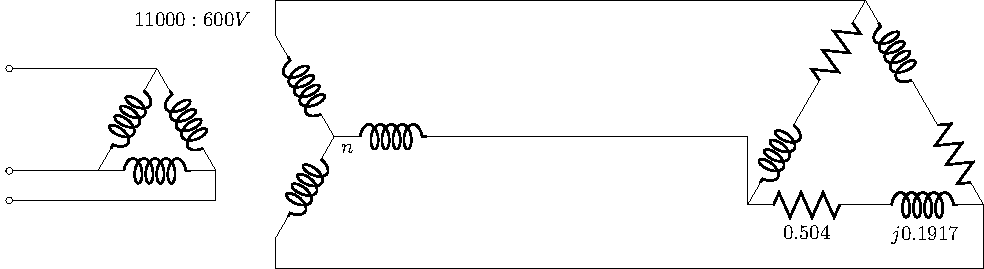
\includegraphics[width=\linewidth]{figTransformersDeltaLoadedExample}
\begin{tikzpicture}[scale=0.75]
%grid
%\draw[gray,thick] (-3,-3) grid (18,5);
%\draw[gray,thin,xstep=0.1,ystep=0.1] (-3,-3) grid (18,5);
%transformer outer dimensions
\pgfmathsetmacro{\shiftX}{9 cm}
\pgfmathsetmacro{\shiftY}{6.5 cm}

\pgfmathsetmacro{\arm}{2}
\pgfmathsetmacro{\con}{2.5}
\pgfmathsetmacro{\conStarS}{\con-\arm*cos(30)}                  %one arm of star is at ninty degree
\pgfmathsetmacro{\conStarL}{\con+\arm*cos(30)}
\pgfmathsetmacro{\h}{sqrt(3)/2*\arm}
\pgfmathsetmacro{\conDeltaS}{\con-\arm/sqrt(3)}                      %one arm of delta is at 90 degree as h=sqrt{3}/2*\arm
\pgfmathsetmacro{\conDeltaL}{\con+\arm/sqrt(12)}
\pgfmathsetmacro{\conDeltaZeroS}{\con-\arm*cos(60)}    %one arm of delta is at 0 degree as h=sqrt{3}/2*\arm
\pgfmathsetmacro{\conDeltaZeroM}{\con}
\pgfmathsetmacro{\conDeltaZeroL}{\con+\arm*cos(60)}


\pgfmathsetmacro{\gap}{3 cm}        %gap between star and delta centres
\pgfmathsetmacro{\startNintyX}{-\h/3}    %start of delta if one arm is at 90 degrees
\pgfmathsetmacro{\startNintyY}{-\arm/2}
\pgfmathsetmacro{\startZeroX}{-\arm/2}   %start of delta if one arm is at 0 degrees
\pgfmathsetmacro{\startZeroY}{-\h/3} 


\node at (0.6,2){$11000:600V$}; 
%DELTA TRANSFORMER
\draw (\startZeroX,\startZeroY)coordinate(delA){} to [inductor] ++(0:\arm)coordinate(delB){} to [inductor] ++(120:\arm)coordinate(delC){} to [inductor] ++(-120:\arm);
\draw (delA) to [short,-o]++(180:\conDeltaZeroS);
\draw (delB) to [short] ++(0,-0.5) to [short,-o]++(180:\conDeltaZeroL);
\draw (delC) to [short,-o]++(180:\conDeltaZeroM);
%STAR TRANSFORMER
\begin{scope}[xshift=\gap]
\draw (0,0)node[below right]{$n$} to [inductor] ++(0:\arm) coordinate(starA){};
\draw (0,0) to [inductor] ++(120:\arm)  to [short] ++(0,0.5) coordinate(starB){};
\draw (0,0) to [inductor] ++(-120:\arm) to [short] ++(0,-0.5)coordinate(starC){};
\end{scope}
%DELTA LOAD
\begin{scope}[xshift=\shiftX]
\draw(2*\startZeroX,2*\startZeroY) coordinate(loadAa){} to [resistor,l_={$0.504$}] ++(0:\arm) to [inductor,l_={$j 0.1917$}] ++(0:\arm)coordinate(loadBb){} to [resistor] ++(120:\arm) to [inductor] ++(120:\arm)coordinate(loadCc){} to [resistor] ++(-120:\arm) to [inductor] ++(-120:\arm);
\end{scope}
\draw (starA) -| (loadAa);
\draw (starB) |- (loadCc);
\draw (starC) -| (loadBb);
\end{tikzpicture}
\caption{ٹرانسفارمر تکونی متوازن بوجھ کو طاقت فراہم کر رہا ہے۔}
\label{شکل_ٹرانسفارمر_تکونی_بار_کی_مثال}
\end{figure}
حل:

پہلے تکونی بوجھ کو ستارہ نما بوجھ میں تبدیل کرتے ہیں
\begin{align*}
Z_Y= \frac{Z_\Delta}{3}=\frac{0.504+j0.1917}{3}=0.168+j0.0639
\end{align*}
اس بوجھ کو ستارہ نما جڑا شکل \حوالہ{شکل_ٹرانسفارمر_تکونی_بار_کو_ستارہ_تبادلہ} میں دکھایا گیا ہے۔اس شکل میں ایک برقی تار جسے نقطہ دار لکیر سے ظاہر کیا گیا ہے کو ٹرانسفارمر کی زمینی نقطہ سے بوجھ کے مشترکہ سرے کے درمیان جڑا دکھایا گیا ہے۔متوازن دور میں اس تار میں برقی رو صفر ہو گی۔حل کرنے کی نیت سے ہم اس متوازن دور سے ایک مرحلہ لے کر حل کرتے ہیں۔
\begin{figure}
\centering
%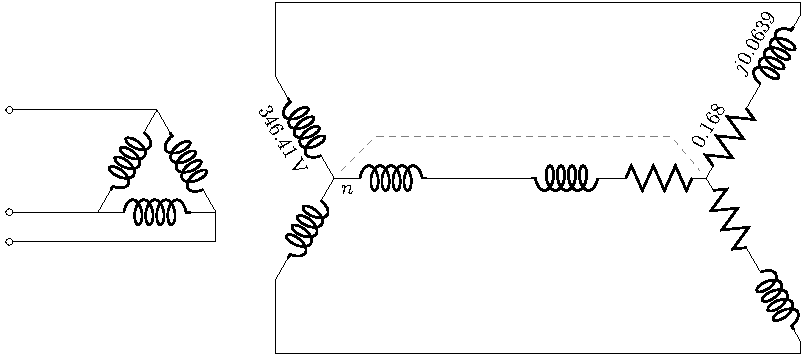
\includegraphics[width=\linewidth]{figTransformersDeltaLoadedExampleTurnedStar}
\begin{tikzpicture}[scale=0.75]
%grid
%\draw[gray,thick] (-3,-3) grid (18,5);
%\draw[gray,thin,xstep=0.1,ystep=0.1] (-3,-3) grid (18,5);
%transformer outer dimensions
\pgfmathsetmacro{\shiftX}{9 cm}
\pgfmathsetmacro{\shiftY}{6.5 cm}

\pgfmathsetmacro{\arm}{2}
\pgfmathsetmacro{\con}{2.5}
\pgfmathsetmacro{\conStarS}{\con-\arm*cos(30)}                  %one arm of star is at ninty degree
\pgfmathsetmacro{\conStarL}{\con+\arm*cos(30)}
\pgfmathsetmacro{\h}{sqrt(3)/2*\arm}
\pgfmathsetmacro{\conDeltaS}{\con-\arm/sqrt(3)}                      %one arm of delta is at 90 degree as h=sqrt{3}/2*\arm
\pgfmathsetmacro{\conDeltaL}{\con+\arm/sqrt(12)}
\pgfmathsetmacro{\conDeltaZeroS}{\con-\arm*cos(60)}    %one arm of delta is at 0 degree as h=sqrt{3}/2*\arm
\pgfmathsetmacro{\conDeltaZeroM}{\con}
\pgfmathsetmacro{\conDeltaZeroL}{\con+\arm*cos(60)}


\pgfmathsetmacro{\gap}{3 cm}        %gap between star and delta centres
\pgfmathsetmacro{\startNintyX}{-\h/3}    %start of delta if one arm is at 90 degrees
\pgfmathsetmacro{\startNintyY}{-\arm/2}
\pgfmathsetmacro{\startZeroX}{-\arm/2}   %start of delta if one arm is at 0 degrees
\pgfmathsetmacro{\startZeroY}{-\h/3} 

%DELTA TRANSFORMER
\draw (\startZeroX,\startZeroY)coordinate(delA){} to [inductor] ++(0:\arm)coordinate(delB){} to [inductor] ++(120:\arm)coordinate(delC){} to [inductor] ++(-120:\arm);
\draw (delA) to [short,-o]++(180:\conDeltaZeroS);
\draw (delB) to [short] ++(0,-0.5) to [short,-o]++(180:\conDeltaZeroL);
\draw (delC) to [short,-o]++(180:\conDeltaZeroM);
%STAR TRANSFORMER
\begin{scope}[xshift=\gap]
\draw (0,0)node[below right]{$n$} to [inductor] ++(0:\arm) coordinate(starA){};
\draw (0,0) to [inductor,l={$\SI{346.41}{\volt}$}] ++(120:\arm)  to [short] ++(0,0.5) coordinate(starB){};
\draw (0,0) to [inductor] ++(-120:\arm) to [short] ++(0,-0.5)coordinate(starC){};
\node at (0,0) (starNN){};
%----------
%STAR LOAD
\begin{scope}[xshift=0.7*\shiftX]
\draw(0,0) to [resistor] ++(180:0.8*\arm) to [inductor] ++(180:0.8*\arm)coordinate(loadA){}; 
\draw(0,0) to [resistor,l_={$0.168$}] ++(60:0.8*\arm) to [inductor,l_={$j 0.0639$}] ++(60:0.8*\arm) to [short] ++(0,0.2)coordinate(loadB){}; 
\draw(0,0) to [resistor] ++(-60:0.8*\arm) to [inductor] ++(-60:0.8*\arm) to [short] ++(0,-0.2) coordinate(loadC){}; 
\draw (starA) -| (loadA);
\draw (starB) |- (loadB);
\draw (starC) |- (loadC);
\node at (0,0) (loadNN){};
\draw[gray,dashed] (starNN) --++(45:1) --++(2.5*\arm,0) --(loadNN);
\end{scope}
\end{scope}
\end{tikzpicture}
\caption{تکونی بوجھ کو مساوی ستارہ بوجھ میں تبدیل کیا گیا ہے۔}
\label{شکل_ٹرانسفارمر_تکونی_بار_کو_ستارہ_تبادلہ}
\end{figure}

یوں مساوی برقی بوجھ میں برقی رو
\begin{align*}
I=\frac{346.41}{0.168+j0.0639}=1927.262\phase{-20.825\degree}
\end{align*}
ہو گی اور اس ایک مرحلہ میں طاقت
\begin{align*}
p=346.41 \times 1927.262 \times \cos (-20.825\degree)=\SI{624007}{\watt}
\end{align*}
ہو گی۔ یوں برقی بوجھ کو پوری درکار برقی طاقت اس کے تین گنا ہو گی یعنی \عددیء{\SI{1872}{\kilo \watt}}  اس بوجھ کا جزو طاقت\حاشیہب{power factor} 
\begin{align*}
\cos (-20.825\degree)=0.93467
\end{align*}
ہے۔

	تکونی بوجھ   میں برقی رو \عددیء{\tfrac{1927.262}{\sqrt{3}}=1112.7} ایمپیئر ہو گی۔ ٹرانسفارمر کی ابتدائی جانب برقی تاروں میں برقی رو
\begin{align*}
\left(\frac{600}{11000} \right) \times 1927.262=105.12
\end{align*}
  ایمپیئر ہو گی۔
\انتہا{مثال}
%
اس مثال میں جزو طاقت \عددیء{0.93467} ہے۔اس کتاب کے لکھتے وقت پاکستان میں اگر صنعتی کارخانوں کی برقی بوجھ کی جزو طاقت \عددیء{0.9} سے کم ہو جائے تو برقی طاقت فراہم کرنے والا ادارہ (واپڈا) جرمانہ نافذ کرتا ہے۔ 

\حصہ{ٹرانسفارمر چالو کرتے لمحہ زیادہ محرکی برقی رو کا گزر}
ہم دیکھ چکے ہیں کہ اگر ٹرانسفارمر کے قالب میں کثافتِ مقناطیسی بہاو سائن نما ہو یعنی \عددیء{B=B_0 \sin \omega t}  تو اس کے لئے ہم لکھ سکتے ہیں
\begin{align*}
v=e=N \frac{\partial \varphi}{\partial t}&=N A_c \frac{\partial B}{\partial t}\\
&=\omega N A_c B_0 \cos \omega t\\
&=V_0 \cos \omega t
\end{align*}
یعنی
\begin{align}\label{مساوات_ٹرانسفارمر_درکار_کثافت_بہاو}
B_0=\frac{V_0}{\omega N A_c}
\end{align}
یہ مساوات برقرار چالو\فرہنگ{برقرار چالو}\حاشیہب{steady state} ٹرانسفارمر کے لئے درست ہے۔

تصور کریں کہ ایک ٹرانسفارمر کو چالو کیا جا رہا ہے۔ چالو ہونے سے پہلے قالب میں مقناطیسی بہاو صفر ہے اور جس لمحہ اسے چالو کیا جائے اس لمحہ بھی یہ صفر ہی رہتا ہے۔	

جس لمحہ ٹرانسفارمر کو چالو کیا جائے اس لمحہ لاگو برقی دباو
\begin{align*}
v=V_0 \cos (\omega t+\theta)
\end{align*}
ہے۔اگر \عددیء{\theta=\pi/2} یہ لمحہ ہو تو آدھے \اصطلاح{دوری عرصہ}\فرہنگ{دوری عرصہ}\حاشیہب{time period}\فرہنگ{time period}  کے بعد قالب میں کثافتِ مقناطیسی بہاو
\begin{align*}
B&=\frac{1}{N A_c} \int_{0}^{\pi/\omega} V_0 \cos (\omega t+\pi/2) \dif t\\
&=\frac{V_0}{\omega N A_c} \sin (\omega t+\pi/2)_0^{\pi/\omega}\\
&=-\left(\frac{2 V_0}{\omega N A_c} \right)
\end{align*}
یعنی کثافتِ مقناطیسی بہاو کا طول معمول سے دگنا ہو گا۔اگر یہی حساب \عددیء{\theta=0} لمحہ کے لئے کیا جائے تو زیادہ سے زیادہ کثافتِ مقناطیسی بہاو بالکل مساوات \حوالہ{مساوات_ٹرانسفارمر_درکار_کثافت_بہاو}  کے عین مطابق ہو گا۔ ان دو زاویوں کے مابین زیادہ سے زیادہ کثافتِ مقناطیسی بہاو ان دو حدوں کے درمیان رہتا ہے۔ 

قالب کی  \عددیء{B-H} خط غیر بتدریج بڑھتا ہے۔لہٰذا \عددیء{B}  دگنا کرنے کی خاطر \عددیء{H} کو کئی گنا بڑھانا ہو گا جو لچھے میں محرک برقی رو بڑھانے سے ہوتا ہے\حاشیہد{\عددیء{2000}  کلو وولٹ-ایمپیئر ٹرانسفارمر سے چالو کرتے وقت تھرتھراہٹ کی آواز آتی ہے}۔یہاں صفحہ \حوالہصفحہ{شکل_مقناطیسی_ادوار_ہیجان_رو_چال_نظرانداز} پر دکھائے  شکل \حوالہ{شکل_مقناطیسی_ادوار_ہیجان_رو_چال_نظرانداز}  سے رجوع کریں۔قوی ٹرانسفارمروں میں ہیجانی کثافتِ مقناطیسی بہاو کی چوٹی \عددیء{1\le B_0\le 1.3} ہوتی ہے۔ٹرانسفارمر چالو کرتے لمحہ یوں کثافتِ مقناطیسی بہاو  \عددیء{2} سے  \عددیء{2.6} ٹسلا تک ہو سکتی ہے جس کے لئے درکار ہیجان انگیز برقی رو نہایت زیادہ ہو گی۔

